\documentclass[11pt, oneside]{book}
%********************************************

\usepackage[phd]{thesisfrontmatter}
%\usepackage[proposal]{thesisfrontmatter}
% For Proposal, uncomment the line "\usepackage[proposal]{thesisfrontmatter}"

%%%%% NEW MATH DEFINITIONS %%%%%

\usepackage{amsmath}
\usepackage{amsfonts}
\usepackage{bm}

% Mark sections of captions for referring to divisions of figures
\newcommand{\figleft}{{\em (Left)}}
\newcommand{\figcenter}{{\em (Center)}}
\newcommand{\figright}{{\em (Right)}}
\newcommand{\figtop}{{\em (Top)}}
\newcommand{\figbottom}{{\em (Bottom)}}
\newcommand{\captiona}{{\em (a)}}
\newcommand{\captionb}{{\em (b)}}
\newcommand{\captionc}{{\em (c)}}
\newcommand{\captiond}{{\em (d)}}

% Highlight a newly defined term
\newcommand{\newterm}[1]{{\bf #1}}


% Figure reference, lower-case.
\def\figref#1{figure~\ref{#1}}
% Figure reference, capital. For start of sentence
\def\Figref#1{Figure~\ref{#1}}
\def\twofigref#1#2{figures \ref{#1} and \ref{#2}}
\def\quadfigref#1#2#3#4{figures \ref{#1}, \ref{#2}, \ref{#3} and \ref{#4}}
% Section reference, lower-case.
\def\secref#1{section~\ref{#1}}
% Section reference, capital.
\def\Secref#1{Section~\ref{#1}}
% Reference to two sections.
\def\twosecrefs#1#2{sections \ref{#1} and \ref{#2}}
% Reference to three sections.
\def\secrefs#1#2#3{sections \ref{#1}, \ref{#2} and \ref{#3}}
% Reference to an equation, lower-case.
\def\eqref#1{equation~\ref{#1}}
% Reference to an equation, upper case
\def\Eqref#1{Equation~\ref{#1}}
% A raw reference to an equation---avoid using if possible
\def\plaineqref#1{\ref{#1}}
% Reference to a chapter, lower-case.
\def\chapref#1{chapter~\ref{#1}}
% Reference to an equation, upper case.
\def\Chapref#1{Chapter~\ref{#1}}
% Reference to a range of chapters
\def\rangechapref#1#2{chapters\ref{#1}--\ref{#2}}
% Reference to an algorithm, lower-case.
\def\algref#1{algorithm~\ref{#1}}
% Reference to an algorithm, upper case.
\def\Algref#1{Algorithm~\ref{#1}}
\def\twoalgref#1#2{algorithms \ref{#1} and \ref{#2}}
\def\Twoalgref#1#2{Algorithms \ref{#1} and \ref{#2}}
% Reference to a part, lower case
\def\partref#1{part~\ref{#1}}
% Reference to a part, upper case
\def\Partref#1{Part~\ref{#1}}
\def\twopartref#1#2{parts \ref{#1} and \ref{#2}}

\def\ceil#1{\lceil #1 \rceil}
\def\floor#1{\lfloor #1 \rfloor}
\def\1{\bm{1}}
\newcommand{\train}{\mathcal{D}}
\newcommand{\valid}{\mathcal{D_{\mathrm{valid}}}}
\newcommand{\test}{\mathcal{D_{\mathrm{test}}}}

\def\eps{{\epsilon}}


% Random variables
\def\reta{{\textnormal{$\eta$}}}
\def\ra{{\textnormal{a}}}
\def\rb{{\textnormal{b}}}
\def\rc{{\textnormal{c}}}
\def\rd{{\textnormal{d}}}
\def\re{{\textnormal{e}}}
\def\rf{{\textnormal{f}}}
\def\rg{{\textnormal{g}}}
\def\rh{{\textnormal{h}}}
\def\ri{{\textnormal{i}}}
\def\rj{{\textnormal{j}}}
\def\rk{{\textnormal{k}}}
\def\rl{{\textnormal{l}}}
% rm is already a command, just don't name any random variables m
\def\rn{{\textnormal{n}}}
\def\ro{{\textnormal{o}}}
\def\rp{{\textnormal{p}}}
\def\rq{{\textnormal{q}}}
\def\rr{{\textnormal{r}}}
\def\rs{{\textnormal{s}}}
\def\rt{{\textnormal{t}}}
\def\ru{{\textnormal{u}}}
\def\rv{{\textnormal{v}}}
\def\rw{{\textnormal{w}}}
\def\rx{{\textnormal{x}}}
\def\ry{{\textnormal{y}}}
\def\rz{{\textnormal{z}}}

% Random vectors
\def\rvepsilon{{\mathbf{\epsilon}}}
\def\rvtheta{{\mathbf{\theta}}}
\def\rva{{\mathbf{a}}}
\def\rvb{{\mathbf{b}}}
\def\rvc{{\mathbf{c}}}
\def\rvd{{\mathbf{d}}}
\def\rve{{\mathbf{e}}}
\def\rvf{{\mathbf{f}}}
\def\rvg{{\mathbf{g}}}
\def\rvh{{\mathbf{h}}}
\def\rvu{{\mathbf{i}}}
\def\rvj{{\mathbf{j}}}
\def\rvk{{\mathbf{k}}}
\def\rvl{{\mathbf{l}}}
\def\rvm{{\mathbf{m}}}
\def\rvn{{\mathbf{n}}}
\def\rvo{{\mathbf{o}}}
\def\rvp{{\mathbf{p}}}
\def\rvq{{\mathbf{q}}}
\def\rvr{{\mathbf{r}}}
\def\rvs{{\mathbf{s}}}
\def\rvt{{\mathbf{t}}}
\def\rvu{{\mathbf{u}}}
\def\rvv{{\mathbf{v}}}
\def\rvw{{\mathbf{w}}}
\def\rvx{{\mathbf{x}}}
\def\rvy{{\mathbf{y}}}
\def\rvz{{\mathbf{z}}}

% Elements of random vectors
\def\erva{{\textnormal{a}}}
\def\ervb{{\textnormal{b}}}
\def\ervc{{\textnormal{c}}}
\def\ervd{{\textnormal{d}}}
\def\erve{{\textnormal{e}}}
\def\ervf{{\textnormal{f}}}
\def\ervg{{\textnormal{g}}}
\def\ervh{{\textnormal{h}}}
\def\ervi{{\textnormal{i}}}
\def\ervj{{\textnormal{j}}}
\def\ervk{{\textnormal{k}}}
\def\ervl{{\textnormal{l}}}
\def\ervm{{\textnormal{m}}}
\def\ervn{{\textnormal{n}}}
\def\ervo{{\textnormal{o}}}
\def\ervp{{\textnormal{p}}}
\def\ervq{{\textnormal{q}}}
\def\ervr{{\textnormal{r}}}
\def\ervs{{\textnormal{s}}}
\def\ervt{{\textnormal{t}}}
\def\ervu{{\textnormal{u}}}
\def\ervv{{\textnormal{v}}}
\def\ervw{{\textnormal{w}}}
\def\ervx{{\textnormal{x}}}
\def\ervy{{\textnormal{y}}}
\def\ervz{{\textnormal{z}}}

% Random matrices
\def\rmA{{\mathbf{A}}}
\def\rmB{{\mathbf{B}}}
\def\rmC{{\mathbf{C}}}
\def\rmD{{\mathbf{D}}}
\def\rmE{{\mathbf{E}}}
\def\rmF{{\mathbf{F}}}
\def\rmG{{\mathbf{G}}}
\def\rmH{{\mathbf{H}}}
\def\rmI{{\mathbf{I}}}
\def\rmJ{{\mathbf{J}}}
\def\rmK{{\mathbf{K}}}
\def\rmL{{\mathbf{L}}}
\def\rmM{{\mathbf{M}}}
\def\rmN{{\mathbf{N}}}
\def\rmO{{\mathbf{O}}}
\def\rmP{{\mathbf{P}}}
\def\rmQ{{\mathbf{Q}}}
\def\rmR{{\mathbf{R}}}
\def\rmS{{\mathbf{S}}}
\def\rmT{{\mathbf{T}}}
\def\rmU{{\mathbf{U}}}
\def\rmV{{\mathbf{V}}}
\def\rmW{{\mathbf{W}}}
\def\rmX{{\mathbf{X}}}
\def\rmY{{\mathbf{Y}}}
\def\rmZ{{\mathbf{Z}}}

% Elements of random matrices
\def\ermA{{\textnormal{A}}}
\def\ermB{{\textnormal{B}}}
\def\ermC{{\textnormal{C}}}
\def\ermD{{\textnormal{D}}}
\def\ermE{{\textnormal{E}}}
\def\ermF{{\textnormal{F}}}
\def\ermG{{\textnormal{G}}}
\def\ermH{{\textnormal{H}}}
\def\ermI{{\textnormal{I}}}
\def\ermJ{{\textnormal{J}}}
\def\ermK{{\textnormal{K}}}
\def\ermL{{\textnormal{L}}}
\def\ermM{{\textnormal{M}}}
\def\ermN{{\textnormal{N}}}
\def\ermO{{\textnormal{O}}}
\def\ermP{{\textnormal{P}}}
\def\ermQ{{\textnormal{Q}}}
\def\ermR{{\textnormal{R}}}
\def\ermS{{\textnormal{S}}}
\def\ermT{{\textnormal{T}}}
\def\ermU{{\textnormal{U}}}
\def\ermV{{\textnormal{V}}}
\def\ermW{{\textnormal{W}}}
\def\ermX{{\textnormal{X}}}
\def\ermY{{\textnormal{Y}}}
\def\ermZ{{\textnormal{Z}}}

% Vectors
\def\vzero{{\bm{0}}}
\def\vone{{\bm{1}}}
\def\vmu{{\bm{\mu}}}
\def\vtheta{{\bm{\theta}}}
\def\va{{\bm{a}}}
\def\vb{{\bm{b}}}
\def\vc{{\bm{c}}}
\def\vd{{\bm{d}}}
\def\ve{{\bm{e}}}
\def\vf{{\bm{f}}}
\def\vg{{\bm{g}}}
\def\vh{{\bm{h}}}
\def\vi{{\bm{i}}}
\def\vj{{\bm{j}}}
\def\vk{{\bm{k}}}
\def\vl{{\bm{l}}}
\def\vm{{\bm{m}}}
\def\vn{{\bm{n}}}
\def\vo{{\bm{o}}}
\def\vp{{\bm{p}}}
\def\vq{{\bm{q}}}
\def\vr{{\bm{r}}}
\def\vs{{\bm{s}}}
\def\vt{{\bm{t}}}
\def\vu{{\bm{u}}}
\def\vv{{\bm{v}}}
\def\vw{{\bm{w}}}
\def\vx{{\bm{x}}}
\def\vy{{\bm{y}}}
\def\vz{{\bm{z}}}

% Elements of vectors
\def\evalpha{{\alpha}}
\def\evbeta{{\beta}}
\def\evepsilon{{\epsilon}}
\def\evlambda{{\lambda}}
\def\evomega{{\omega}}
\def\evmu{{\mu}}
\def\evpsi{{\psi}}
\def\evsigma{{\sigma}}
\def\evtheta{{\theta}}
\def\eva{{a}}
\def\evb{{b}}
\def\evc{{c}}
\def\evd{{d}}
\def\eve{{e}}
\def\evf{{f}}
\def\evg{{g}}
\def\evh{{h}}
\def\evi{{i}}
\def\evj{{j}}
\def\evk{{k}}
\def\evl{{l}}
\def\evm{{m}}
\def\evn{{n}}
\def\evo{{o}}
\def\evp{{p}}
\def\evq{{q}}
\def\evr{{r}}
\def\evs{{s}}
\def\evt{{t}}
\def\evu{{u}}
\def\evv{{v}}
\def\evw{{w}}
\def\evx{{x}}
\def\evy{{y}}
\def\evz{{z}}

% Matrix
\def\mA{{\bm{A}}}
\def\mB{{\bm{B}}}
\def\mC{{\bm{C}}}
\def\mD{{\bm{D}}}
\def\mE{{\bm{E}}}
\def\mF{{\bm{F}}}
\def\mG{{\bm{G}}}
\def\mH{{\bm{H}}}
\def\mI{{\bm{I}}}
\def\mJ{{\bm{J}}}
\def\mK{{\bm{K}}}
\def\mL{{\bm{L}}}
\def\mM{{\bm{M}}}
\def\mN{{\bm{N}}}
\def\mO{{\bm{O}}}
\def\mP{{\bm{P}}}
\def\mQ{{\bm{Q}}}
\def\mR{{\bm{R}}}
\def\mS{{\bm{S}}}
\def\mT{{\bm{T}}}
\def\mU{{\bm{U}}}
\def\mV{{\bm{V}}}
\def\mW{{\bm{W}}}
\def\mX{{\bm{X}}}
\def\mY{{\bm{Y}}}
\def\mZ{{\bm{Z}}}
\def\mBeta{{\bm{\beta}}}
\def\mPhi{{\bm{\Phi}}}
\def\mLambda{{\bm{\Lambda}}}
\def\mSigma{{\bm{\Sigma}}}

% Tensor
\DeclareMathAlphabet{\mathsfit}{\encodingdefault}{\sfdefault}{m}{sl}
\SetMathAlphabet{\mathsfit}{bold}{\encodingdefault}{\sfdefault}{bx}{n}
\newcommand{\tens}[1]{\bm{\mathsfit{#1}}}
\def\tA{{\tens{A}}}
\def\tB{{\tens{B}}}
\def\tC{{\tens{C}}}
\def\tD{{\tens{D}}}
\def\tE{{\tens{E}}}
\def\tF{{\tens{F}}}
\def\tG{{\tens{G}}}
\def\tH{{\tens{H}}}
\def\tI{{\tens{I}}}
\def\tJ{{\tens{J}}}
\def\tK{{\tens{K}}}
\def\tL{{\tens{L}}}
\def\tM{{\tens{M}}}
\def\tN{{\tens{N}}}
\def\tO{{\tens{O}}}
\def\tP{{\tens{P}}}
\def\tQ{{\tens{Q}}}
\def\tR{{\tens{R}}}
\def\tS{{\tens{S}}}
\def\tT{{\tens{T}}}
\def\tU{{\tens{U}}}
\def\tV{{\tens{V}}}
\def\tW{{\tens{W}}}
\def\tX{{\tens{X}}}
\def\tY{{\tens{Y}}}
\def\tZ{{\tens{Z}}}


% Graph
\def\gA{{\mathcal{A}}}
\def\gB{{\mathcal{B}}}
\def\gC{{\mathcal{C}}}
\def\gD{{\mathcal{D}}}
\def\gE{{\mathcal{E}}}
\def\gF{{\mathcal{F}}}
\def\gG{{\mathcal{G}}}
\def\gH{{\mathcal{H}}}
\def\gI{{\mathcal{I}}}
\def\gJ{{\mathcal{J}}}
\def\gK{{\mathcal{K}}}
\def\gL{{\mathcal{L}}}
\def\gM{{\mathcal{M}}}
\def\gN{{\mathcal{N}}}
\def\gO{{\mathcal{O}}}
\def\gP{{\mathcal{P}}}
\def\gQ{{\mathcal{Q}}}
\def\gR{{\mathcal{R}}}
\def\gS{{\mathcal{S}}}
\def\gT{{\mathcal{T}}}
\def\gU{{\mathcal{U}}}
\def\gV{{\mathcal{V}}}
\def\gW{{\mathcal{W}}}
\def\gX{{\mathcal{X}}}
\def\gY{{\mathcal{Y}}}
\def\gZ{{\mathcal{Z}}}

% Sets
\def\sA{{\mathbb{A}}}
\def\sB{{\mathbb{B}}}
\def\sC{{\mathbb{C}}}
\def\sD{{\mathbb{D}}}
% Don't use a set called E, because this would be the same as our symbol
% for expectation.
\def\sF{{\mathbb{F}}}
\def\sG{{\mathbb{G}}}
\def\sH{{\mathbb{H}}}
\def\sI{{\mathbb{I}}}
\def\sJ{{\mathbb{J}}}
\def\sK{{\mathbb{K}}}
\def\sL{{\mathbb{L}}}
\def\sM{{\mathbb{M}}}
\def\sN{{\mathbb{N}}}
\def\sO{{\mathbb{O}}}
\def\sP{{\mathbb{P}}}
\def\sQ{{\mathbb{Q}}}
\def\sR{{\mathbb{R}}}
\def\sS{{\mathbb{S}}}
\def\sT{{\mathbb{T}}}
\def\sU{{\mathbb{U}}}
\def\sV{{\mathbb{V}}}
\def\sW{{\mathbb{W}}}
\def\sX{{\mathbb{X}}}
\def\sY{{\mathbb{Y}}}
\def\sZ{{\mathbb{Z}}}

% Entries of a matrix
\def\emLambda{{\Lambda}}
\def\emA{{A}}
\def\emB{{B}}
\def\emC{{C}}
\def\emD{{D}}
\def\emE{{E}}
\def\emF{{F}}
\def\emG{{G}}
\def\emH{{H}}
\def\emI{{I}}
\def\emJ{{J}}
\def\emK{{K}}
\def\emL{{L}}
\def\emM{{M}}
\def\emN{{N}}
\def\emO{{O}}
\def\emP{{P}}
\def\emQ{{Q}}
\def\emR{{R}}
\def\emS{{S}}
\def\emT{{T}}
\def\emU{{U}}
\def\emV{{V}}
\def\emW{{W}}
\def\emX{{X}}
\def\emY{{Y}}
\def\emZ{{Z}}
\def\emSigma{{\Sigma}}

% entries of a tensor
% Same font as tensor, without \bm wrapper
\newcommand{\etens}[1]{\mathsfit{#1}}
\def\etLambda{{\etens{\Lambda}}}
\def\etA{{\etens{A}}}
\def\etB{{\etens{B}}}
\def\etC{{\etens{C}}}
\def\etD{{\etens{D}}}
\def\etE{{\etens{E}}}
\def\etF{{\etens{F}}}
\def\etG{{\etens{G}}}
\def\etH{{\etens{H}}}
\def\etI{{\etens{I}}}
\def\etJ{{\etens{J}}}
\def\etK{{\etens{K}}}
\def\etL{{\etens{L}}}
\def\etM{{\etens{M}}}
\def\etN{{\etens{N}}}
\def\etO{{\etens{O}}}
\def\etP{{\etens{P}}}
\def\etQ{{\etens{Q}}}
\def\etR{{\etens{R}}}
\def\etS{{\etens{S}}}
\def\etT{{\etens{T}}}
\def\etU{{\etens{U}}}
\def\etV{{\etens{V}}}
\def\etW{{\etens{W}}}
\def\etX{{\etens{X}}}
\def\etY{{\etens{Y}}}
\def\etZ{{\etens{Z}}}

% The true underlying data generating distribution
\newcommand{\pdata}{p_{\rm{data}}}
% The empirical distribution defined by the training set
\newcommand{\ptrain}{\hat{p}_{\rm{data}}}
\newcommand{\Ptrain}{\hat{P}_{\rm{data}}}
% The model distribution
\newcommand{\pmodel}{p_{\rm{model}}}
\newcommand{\Pmodel}{P_{\rm{model}}}
\newcommand{\ptildemodel}{\tilde{p}_{\rm{model}}}
% Stochastic autoencoder distributions
\newcommand{\pencode}{p_{\rm{encoder}}}
\newcommand{\pdecode}{p_{\rm{decoder}}}
\newcommand{\precons}{p_{\rm{reconstruct}}}

\newcommand{\laplace}{\mathrm{Laplace}} % Laplace distribution

\newcommand{\E}{\mathbb{E}}
\newcommand{\Ls}{\mathcal{L}}
\newcommand{\R}{\mathbb{R}}
\newcommand{\emp}{\tilde{p}}
\newcommand{\lr}{\alpha}
\newcommand{\reg}{\lambda}
\newcommand{\rect}{\mathrm{rectifier}}
\newcommand{\softmax}{\mathrm{softmax}}
\newcommand{\sigmoid}{\sigma}
\newcommand{\softplus}{\zeta}
\newcommand{\KL}{D_{\mathrm{KL}}}
\newcommand{\Var}{\mathrm{Var}}
\newcommand{\standarderror}{\mathrm{SE}}
\newcommand{\Cov}{\mathrm{Cov}}
% Wolfram Mathworld says $L^2$ is for function spaces and $\ell^2$ is for vectors
% But then they seem to use $L^2$ for vectors throughout the site, and so does
% wikipedia.
\newcommand{\normlzero}{L^0}
\newcommand{\normlone}{L^1}
\newcommand{\normltwo}{L^2}
\newcommand{\normlp}{L^p}
\newcommand{\normmax}{L^\infty}

\newcommand{\parents}{Pa} % See usage in notation.tex. Chosen to match Daphne's book.

\DeclareMathOperator*{\argmax}{arg\,max}
\DeclareMathOperator*{\argmin}{arg\,min}

\DeclareMathOperator{\sign}{sign}
\DeclareMathOperator{\Tr}{Tr}
\let\ab\allowbreak


\newcommand{\cX}{\mathcal{X}}
\newcommand{\cD}{\mathcal{D}}


\setlength{\parindent}{0pt}
\usepackage{booktabs}
\usepackage{amsmath} % math extensions
\usepackage{amsfonts} %...and ams math fonts
\usepackage{multicol} % Allow spanning cells in tables
\usepackage{graphics} % .jpg, .png, .pdf image import 
% automatically sorts citations; comment to disable
\usepackage[sort,nocompress]{cite} 
\usepackage[toc,page]{appendix} % for appendices
% \usepackage[margin=1.0in]{geometry}
\usepackage{geometry}
\usepackage[hyphens]{url}
\usepackage{natbib}
% \usepackage{url}
\usepackage{graphicx}
\usepackage{subfigure}
\usepackage{booktabs} % for professional tables
% For theorems and such
\usepackage{amsmath}
\usepackage{amssymb}
\usepackage{mathtools}
\usepackage{amsthm}
\usepackage{placeins}
\theoremstyle{plain}
\newtheorem{theorem}{Theorem}[section]
\newtheorem{proposition}[theorem]{Proposition}
\newtheorem{lemma}[theorem]{Lemma}
\newtheorem{corollary}[theorem]{Corollary}
\theoremstyle{definition}
\newtheorem{definition}[theorem]{Definition}
\newtheorem{assumption}[theorem]{Assumption}
\newtheorem{method}[theorem]{Method}
\theoremstyle{remark}
\newtheorem{remark}[theorem]{Remark}
\usepackage{wrapfig}
\usepackage{xcolor}
\usepackage{colortbl}
\usepackage{tikz}
\usetikzlibrary{positioning,shapes,arrows,calc,fit}
\usepackage{algorithm}
\usepackage{algpseudocode}
\begin{document}

%*******************************************
% FRONT MATTER
%*******************************************
\pagenumbering{roman}
\degreetitle{[Proposal Title {\bf OR} Dissertation Title as it appears on the Dissertation Certificate]}

\degreeauthor{[professional name of author]}

\degreedate{[Month and year of
Dissertation Acceptance was signed]}

%\prevdegreeA{B.S. Penn State University, 1994}

%\prevdegreeB{M.S. Stony Brook University, 1998}

\advisor{[Advisor's name]}

\memberA{[Committee member's name]}
\memberB{[Committee member's name]}
\memberC{[Committee member's name]}
\memberD{[Ph.D. Program Director name]}
\externalchair{[External Chair's name]}

%********************************************
% FOR PROPOSAL, uncomment the following lines
%\makeproposaldeclaration
%\makePHDproposalapproval

% FOR THESIS
\makedeclaration
\makeapproval
\makecopyright
%********************************************


\begin{abstract}
This is the abstract text with no more than 350 words.

\end{abstract}
\begin{acknowledgements}
This is the acknowledgements text
\end{acknowledgements}
\begin{dedication}

This is the dedication text
\end{dedication}

% TABLE OF CONTENTS + LISTS OF FIGS/TABLES
\tableofcontents
\listoffigures
\listoftables

% Hack: make sure arabic numerals start
% on first page of the introduction.
\pagebreak
\pagenumbering{arabic}

%*******************************************
% MAIN TEXT
%*******************************************

% Chapters of the document 
% (in separate .tex files)
\chapter{Introduction}

The deployment of machine learning systems in real-world applications has revealed a critical challenge: the ability to recognize when a model encounters inputs that fall outside its training distribution. This challenge, known as out-of-distribution (OOD) detection, has become increasingly important as machine learning systems are deployed in safety-critical domains such as healthcare, autonomous driving, and financial services. When models encounter unfamiliar inputs, they often produce overconfident predictions that can lead to dangerous consequences, highlighting the urgent need for reliable uncertainty quantification and OOD detection mechanisms.

The fundamental problem lies in the inherent limitations of supervised learning paradigms, which excel at making predictions within the distribution of their training data but struggle to recognize their own knowledge boundaries. Traditional machine learning models are trained to minimize prediction error on a fixed set of classes or tasks, but they lack the ability to identify when test inputs represent entirely new categories, domains, or scenarios that were not present during training \citep{hendrycks2016baseline}. This limitation becomes particularly problematic in open-world settings where the assumption of a closed, well-defined input space is violated.

Recent advances in deep learning have exacerbated this challenge while simultaneously providing new opportunities for solutions. Large-scale neural networks, particularly transformer-based language models, demonstrate remarkable capabilities in learning complex patterns and generating human-like responses. However, these same models are prone to hallucinations—generating plausible-sounding but factually incorrect or unverifiable content \citep{li2023halueval,lin2021truthfulqa}. The intersection of OOD detection and hallucination detection represents a critical frontier in ensuring the reliability and safety of modern AI systems \citep{huang2020survey}.

\section{Problem Statement and Motivation}

This dissertation addresses three fundamental challenges in the reliable deployment of machine learning systems: (1) the failure of existing OOD detection methods in single-domain settings where domain-specific features are discarded during training, (2) the limitations of unlabeled OOD detection approaches that ignore critical label information, and (3) the lack of principled information-theoretic frameworks for understanding and detecting hallucinations in large language models.

The first challenge emerges from a phenomenon we term \emph{domain feature collapse}, where supervised learning models trained on single-domain datasets learn to discard domain-specific features in favor of class-specific features. This creates dangerous blind spots in OOD detection, as models cannot distinguish between in-domain and out-of-domain samples that share similar class features. For example, a medical imaging model trained exclusively on X-ray images may confidently classify MRI scans of the same anatomical structures, despite the fundamental difference in imaging modality.

The second challenge concerns the growing interest in unlabeled OOD detection methods that aim to detect distributional shifts without relying on supervised learning objectives. While these approaches offer theoretical elegance and practical advantages in scenarios where labels are expensive or unavailable, they suffer from a fundamental limitation we term \emph{label blindness}. When the features learned by unsupervised or self-supervised methods are independent of the features relevant for the target classification task, OOD detection performance degrades significantly, particularly in scenarios where OOD samples share semantic similarity with in-distribution data.

The third challenge addresses the critical need for principled approaches to hallucination detection in large language models. Despite significant progress in developing language models with impressive capabilities, these systems frequently generate content that appears plausible but lacks factual grounding. Existing approaches to hallucination detection rely primarily on post-hoc analysis or external verification systems, but lack theoretical frameworks for understanding why hallucinations occur and how they can be predicted or prevented.

\section{Research Objectives and Contributions}

This dissertation proposes to advance the state of knowledge in OOD detection and hallucination detection through three primary research objectives, each addressing one of the fundamental challenges outlined above.

\textbf{Objective 1: Theoretical Analysis and Mitigation of Domain Feature Collapse}

We aim to provide the first comprehensive theoretical characterization of domain feature collapse in single-domain OOD detection settings. Through information-theoretic analysis, we will prove that supervised learning models inevitably discard domain-specific features when trained on single-domain datasets, leading to systematic failures in OOD detection. We will develop and validate domain filtering techniques that can mitigate these failures by explicitly preserving domain-relevant information during the detection process.

Our theoretical contributions will include formal definitions of domain features and their relationship to class features, mathematical proofs demonstrating the inevitability of domain feature collapse under standard supervised learning objectives, and analysis of the conditions under which domain filtering can restore effective OOD detection performance. The practical contributions will include novel two-stage detection frameworks that combine domain-level and class-level detection mechanisms.

\textbf{Objective 2: Understanding and Addressing Label Blindness in Unlabeled OOD Detection}

We will develop a comprehensive theoretical framework for understanding when and why unlabeled OOD detection methods fail, with particular focus on the label blindness phenomenon. Through information-theoretic analysis, we will characterize the conditions under which unsupervised learning objectives capture features that are independent of the target classification task, leading to systematic OOD detection failures.

Our contributions will include the introduction of Adjacent OOD detection as a novel evaluation paradigm that captures the theoretically predicted failures of unlabeled methods, comprehensive empirical validation across multiple datasets and architectures, and theoretical analysis of the fundamental limitations of label-agnostic approaches. We will also explore hybrid approaches that combine supervised and unsupervised objectives to mitigate label blindness while preserving the advantages of unlabeled methods.

\textbf{Objective 3: Information-Theoretic Framework for Hallucination Detection}

We propose to develop the first comprehensive information-theoretic framework for understanding and detecting hallucinations in large language models. Our central hypothesis is that hallucinations arise from insufficient mutual information between input queries and generated responses, particularly in the intermediate layers of transformer architectures. We will develop novel contrastive mutual information estimation methods specifically designed for analyzing information flow in question-answering contexts.

Our theoretical contributions will include formal definitions of hallucinations in terms of information-theoretic quantities, analysis of how mutual information degrades across transformer layers, and identification of critical information bottlenecks that predict hallucination emergence. The practical contributions will include novel detection methods based on layer-wise mutual information analysis and validation across multiple language model architectures and hallucination benchmarks.

\section{Methodology and Approach}

Our research methodology combines rigorous theoretical analysis with comprehensive empirical validation across multiple domains and datasets. We employ information theory as the unifying mathematical framework for understanding the fundamental limitations and opportunities in both OOD detection and hallucination detection \citep{shannon1948mathematical,cover1999elements}.

For the theoretical analysis, we leverage tools from information theory, including mutual information, entropy, and the information bottleneck principle \citep{tishby2000information}, to characterize the conditions under which detection methods succeed or fail. We develop formal mathematical proofs that establish fundamental limitations of existing approaches and identify the theoretical foundations for improved methods.

The empirical validation encompasses both controlled synthetic experiments and real-world applications across diverse domains including computer vision, natural language processing, and specialized applications such as medical imaging and satellite imagery. We employ standardized benchmarks where available and develop novel evaluation protocols where existing benchmarks are insufficient to capture the theoretical phenomena we investigate.

Our experimental design emphasizes reproducibility and statistical rigor, employing multiple random seeds, cross-validation, and bootstrap sampling to ensure robust conclusions. We conduct comprehensive ablation studies to isolate the contributions of different components and validate the generalizability of our findings across different model architectures, scales, and training paradigms.

\section{Dissertation Organization}

This dissertation is organized into six main chapters that systematically address the research objectives outlined above. Chapter 2 provides comprehensive background on the theoretical foundations, including detailed coverage of out-of-distribution detection, information theory, and hallucination detection in large language models. Chapter 3 presents a thorough literature review that positions our work within the broader context of uncertainty quantification, representation learning, and language model safety.

Chapters 4 and 5 present our primary research contributions addressing domain feature collapse and label blindness respectively. Chapter 4 focuses on single-domain OOD detection, providing theoretical analysis of domain feature collapse and empirical validation of domain filtering approaches. Chapter 5 addresses unlabeled OOD detection, introducing the label blindness theorem and the Adjacent OOD evaluation paradigm.

Chapter 6 presents our proposed research on hallucination detection through information-theoretic analysis, including the development of contrastive mutual information estimation methods and their application to understanding information flow in transformer architectures. Chapter 7 outlines a detailed research timeline for completing the proposed work, and Chapter 8 provides conclusions and discusses the broader implications of our research for the reliable deployment of machine learning systems.

\section{Expected Impact and Significance}

This research addresses fundamental challenges in the safe and reliable deployment of machine learning systems, with implications spanning both theoretical understanding and practical applications. The theoretical contributions advance our understanding of the fundamental limitations of existing approaches, providing mathematical frameworks that can guide the development of more robust and reliable systems.

The practical contributions offer immediate benefits for practitioners deploying machine learning systems in real-world applications. The domain filtering techniques developed for single-domain OOD detection can improve the safety of specialized applications such as medical diagnosis and industrial monitoring. The insights into label blindness can guide the selection and design of OOD detection methods for scenarios where labeled data is scarce or expensive.

The information-theoretic framework for hallucination detection addresses one of the most pressing challenges in the deployment of large language models, providing tools for understanding, predicting, and mitigating the generation of factually incorrect content. This work has particular relevance for applications where factual accuracy is critical, such as educational systems, medical question-answering, and scientific literature analysis.

More broadly, this research contributes to the growing field of AI safety by providing principled approaches to uncertainty quantification and failure detection in modern machine learning systems. The information-theoretic perspective offers a unifying framework that can be applied across different domains and architectures, potentially influencing the design of future AI systems that are inherently more robust and reliable.

\chapter{Background and Definitions}

\section{Out of Distribution Detection}

Out-of-distribution (OOD) detection addresses a critical challenge in modern machine learning: the ability to recognize when a model is presented with inputs that fall outside the scope of what it has been trained to understand. While supervised models excel at making predictions within the distribution of their training data, they are notoriously prone to overconfident predictions when confronted with novel or unexpected inputs — sometimes with dangerous consequences, especially in high-stakes applications such as healthcare, autonomous driving, or security systems.

The task of out-of-distribution detection is to identify a semantic shift in the data \citep{yang2021generalized}. This is determining when no predicted label could match the true label $\vy \notin \sY_{in}$, where $\sY_{in}$ represents the set of in-distribution training labels. In this case, we would consider the semantic space of the sample and the training distribution to be different, representing a semantic shift. We can express the probability that a sample is out-of-distribution via $P(\vy \notin \sY_{in} | \vx)$. 

\begin{definition}
    Out-of-Distribution (OOD) Detection: Given an input $\rvx$ and a set of in-distribution labels $\sY_{\text{in}}$, OOD detection is the task of identifying whether the true label $\rvy$ belongs outside the in-distribution set, i.e., $\rvy \notin \sY_{\text{in}}$, or equivalently estimating $P(\rvy \notin \sY_{\text{in}} \mid \rvx)$.
    \label{defineood}
    \vspace{-2mm}
\end{definition}

One baseline approach to estimate this probability is the \textit{Maximum Softmax Probability (MSP)} method. Here, a trained classifier outputs softmax probabilities across known classes, and the maximum probability $\texttt{MSP}(\mathbf{x})$ is interpreted as a confidence score. A low maximum confidence suggests that the input might not belong to any known class, leading to the simple baseline:

\begin{method}[Maximum Softmax Probability (MSP)]
Given an input $\mathbf{x}$, the MSP method estimates the probability of being out-of-distribution as $1 - \texttt{MSP}(\mathbf{x})$, where $\texttt{MSP}(\mathbf{x}) = \max_{y \in \mathcal{Y}_{\text{in}}} P(y \mid \mathbf{x})$.
\label{methodmsp}
\end{method}

Furthermore, we are only concerned with labels that can be generated using only $\rvx$, via function $f$ which depends solely on $\rvx$ and no other information. $f_\rvy$ may represent human labelers that generate $\rvy$. If we consider $\sY_{all}$ as the set of all possible labels that can be generated from $f_\rvy(\rvx \in \sX_{all})$, a subset of $\sX_{all}$ considered as $\sX_{training}$ may not contain all labels in $\sY_{all}$. For real world datasets, it is possible that $\sY_{in} \subsetneq \sY_{all}$.



While related to other concepts like \textit{anomaly detection}, OOD detection is distinct in key ways. Anomaly detection usually focuses on rare or abnormal data points \textit{within} the same distribution (e.g., detecting fraudulent transactions), whereas OOD detection focuses on recognizing inputs from \textit{entirely different} distributions or classes, outside the model’s prior knowledge. Furthermore, OOD detection primarily targets \textit{epistemic uncertainty} — the model’s uncertainty due to limited knowledge — rather than \textit{aleatoric uncertainty}, which arises from inherent noise or variability in the data.

Practically, OOD detection methods fall into two broad categories:
\begin{itemize}
    \item \textbf{Training-agnostic approaches}, like MSP or entropy-based scoring, which apply directly to existing classifiers without altering their training process.
    \item \textbf{Training-aware approaches}, which adapt model architectures, loss functions, or data augmentation strategies specifically to improve OOD recognition capabilities.
\end{itemize}

Evaluation typically involves exposing the model to benchmark OOD datasets designed to test its ability to reject or abstain from confident predictions on unfamiliar samples, while maintaining strong performance on in-distribution data. Additional information regarding methods and benchmarks will be provided in a later section. 


\section{Anomaly Detection}

Although anomaly detection and out-of-distribution (OOD) detection are sometimes used interchangeably in the literature, they address fundamentally different problems, with distinct assumptions, goals, and evaluation settings.

\subsection{Definiton and Scope}

Anomaly detection focuses on identifying individual data points that deviate significantly from the expected patterns within a single dataset or distribution. These anomalies, or outliers, are typically rare and often correspond to noise, rare events, or fraudulent activities within the same domain as the training data. For example, anomaly detection might flag fraudulent transactions in a credit card dataset, where the system has only ever seen transaction records from that specific financial context.

OOD detection, on the other hand, aims to detect data that comes from a different distribution altogether — one that was not seen during training. It concerns the model’s ability to recognize when a test input belongs to a class, domain, or environment that falls outside the model’s learned distribution. For example, an image classifier trained only on animals should ideally flag an image of a car as OOD, even though the car is not necessarily anomalous within its own context.

\subsection{Training Assumptions}

Anomaly detection methods typically assume access only to normal (non-anomalous) data during training and must learn to recognize deviations without ever seeing examples of the anomalies. This is often referred to as a one-class learning problem.

In contrast, OOD detection typically operates in a supervised learning context where the model has been trained on multiple in-distribution classes, and the challenge is to detect test inputs that fall outside this known set. Here, the focus is on recognizing the model’s epistemic uncertainty — i.e., knowing what the model doesn’t know.

\subsection{Evaluation Settings}

Anomaly detection is typically evaluated using synthetic or labeled anomaly datasets, where the goal is to identify rare but known outlier patterns within the same dataset.

OOD detection is evaluated by exposing the model to entirely new datasets or domains and measuring its ability to correctly reject or abstain from making confident predictions on these unfamiliar inputs. This setting often requires curated OOD benchmark datasets distinct from the in-distribution training data.

\section{Information Theory}

Information theory provides a mathematical framework for quantifying uncertainty, information content, and the relationships between random variables. Originally developed by \citet{shannon1948mathematical}, it has become foundational for many areas of machine learning, including uncertainty quantification, representation learning, and out-of-distribution (OOD) detection. The following are various definitions that are critical to understanding information theory.


\begin{definition}
\textbf{Entropy}: The entropy of a discrete random variable $\rvx$ with distribution $p(\vx)$ is defined as the expected amount of uncertainty or information contained in $\rvx$, denoted by $H(\rvx)$.
\label{def:entropy}
\end{definition}

\begin{definition}
\textbf{Conditional Entropy}: The conditional entropy $H(\rvy \mid \rvx)$ measures the remaining uncertainty in a random variable $\rvy$ given knowledge of another random variable $\rvx$.
\label{def:conditional_entropy}
\end{definition}

\begin{definition}
\textbf{Mutual Information}: The mutual information between random variables $\rvx$ and $\rvy$, denoted $I(\rvx; \rvy)$, quantifies the amount of information shared between $\rvx$ and $\rvy$, or equivalently, the reduction in uncertainty about $\rvx$ given knowledge of $\rvy$.
\label{def:mutual_information}
\end{definition}

\begin{definition}
\textbf{Kullback-Leibler (KL) Divergence}: The KL divergence between two distributions $P$ and $Q$, denoted $D_{\mathrm{KL}}(P \parallel Q)$, measures how much the distribution $P$ diverges from the reference distribution $Q$.
\label{def:kl_divergence}
\end{definition}

\begin{definition}
\textbf{Chain Rule for Entropy}: The joint entropy of two random variables $\rvx$ and $\rvy$ satisfies the chain rule:
\[
H(\rvx, \rvy) = H(\rvx) + H(\rvy \mid \rvx),
\]
expressing that the total uncertainty can be decomposed into the uncertainty of $\rvx$ plus the uncertainty of $\rvy$ given $\rvx$.
\label{def:chain_rule}
\end{definition}

\begin{definition}
\textbf{Mutual Information as KL Divergence}: The mutual information between $\rvx$ and $\rvy$ can be equivalently defined as the KL divergence between the joint distribution $p(\vx, \vy)$ and the product of the marginals $p(\vx)p(\vy)$:
\[
I(\rvx; \rvy) = D_{\mathrm{KL}}(p(\vx, \vy) \parallel p(\vx)p(\vy)).
\]
\label{def:mi_kl}
\end{definition}

\begin{definition}
\textbf{Non-negativity of Mutual Information}: Mutual information is always non-negative, that is, $I(\rvx; \rvy) \geq 0$, with equality if and only if $\rvx$ and $\rvy$ are independent.
\label{def:nonneg_mi}
\end{definition}

\begin{definition}
\textbf{Chain Rule for Mutual Information}: The mutual information between two random variables $\rvx$ and $\rvy$ can be decomposed using the chain rule as follows:
\[
I(\rvx; \rvy) = I(\rvx; \rvz) + I(\rvz; \rvy \mid \rvx),
\]
where $\rvz$ is a third variable, and $I(\rvx; \rvy)$ represents the total mutual information between $\rvx$ and $\rvy$. This decomposition expresses the amount of shared information in terms of intermediate variables that mediate the relationship.
\label{def:chain_rule_mi}
\end{definition}

\subsection{Entropy and Mutual Information}

Entropy and mutual information are central concepts in information theory, and they play a key role in understanding uncertainty and information flow in machine learning models. 

\textbf{Entropy}, as defined in Definition \ref{def:entropy}, measures the average uncertainty in a random variable $\rvx$. It quantifies how much unpredictability exists in the outcomes of $\rvx$. In machine learning, entropy is often used to assess the uncertainty in a model's predictions or to regularize a model by minimizing its uncertainty.

\textbf{Mutual information}, as defined in Definition \ref{def:mutual_information}, measures the amount of information shared between two random variables, $\rvx$ and $\rvy$. Specifically, it quantifies how much knowing one variable reduces uncertainty about the other. In machine learning, mutual information is used to gauge the relevance of features to the target variable, aiding in feature selection and representation learning. By maximizing mutual information between representations and labels, we can improve the expressiveness and usefulness of learned features.

\section{Information Bottleneck and Minimal Sufficient Statistic}

In this section, we introduce two important concepts in information theory that are relevant for understanding how to efficiently represent information while preserving relevant information: the **Information Bottleneck** and the **Minimal Sufficient Statistic**.


\subsection{Minimal Sufficient Statistic}

A **Minimal Sufficient Statistic** is a concept from statistics that defines a statistic that captures all the information about a parameter of interest in a dataset while being the most compact representation. In the context of information theory, it is the statistic that minimizes the loss of information and is often used in maximum likelihood estimation (MLE).

\begin{definition}
\textbf{Minimal Sufficient Statistic}: A statistic \( T(\rvx) \) is called a \textit{minimal sufficient statistic} for a random variable \( \rvx \) with respect to a parameter \( \rvy \) if it satisfies the following two conditions:
\begin{itemize}
    \item \textbf{Sufficiency}: \( T(\rvx) \) is sufficient for \( \rvy \), meaning that it captures all the information about \( \rvy \) contained in \( \rvx \), i.e., 
    \[
    I(\rvx; \rvy \mid T(\rvx)) = 0.
    \]
    \item \textbf{Minimality}: There exists no other statistic \( s \) such that \( s \) is sufficient for \( \rvy \) and \( s \) is a function of \( T(\rvx) \), i.e., there exists a function \( f(s) \) such that \( s = f(T(\rvx)) \).
\end{itemize}
Formally, the minimal sufficient statistic \( T(\rvx) \) is the statistic that retains all the relevant information about \( \rvy \) and satisfies the condition that for any other sufficient statistic \( s \), there exists an \( f(s) \) such that \( s = f(T(\rvx)) \), making \( T(\rvx) \) the minimal sufficient statistic.
\label{def:mss}
\end{definition}

The **Minimal Sufficient Statistic** is crucial in statistical inference because it ensures that no further information about the parameter $\theta$ can be extracted from the data, given the statistic $T(\rvx)$. It is often used in the context of parameter estimation where the goal is to reduce the data to the smallest possible set that still retains all necessary information for accurate inference.

\subsection{Information Bottleneck}

The Information Bottleneck (IB) principle, introduced by \cite{tishby2000information}, provides a framework for learning representations of data that capture the most relevant information while discarding unnecessary details. The core idea of the Information Bottleneck is to find a representation of a random variable $\rvx$ that preserves the information about a target variable $\rvy$, but minimizes the amount of information retained about irrelevant variables. Effectively, we expect a model's representation $\rvz$ to compress towards the minimal sufficient statistic, as per definition \ref{def:mss}, under information bottleneck optimization.

\begin{definition}
\textbf{Information Bottleneck}: Given two random variables $\rvx$ and $\rvy$, the goal of the Information Bottleneck is to find a representation $\rvz$ of $\rvx$ such that the mutual information $I(\rvz; \rvy)$ is maximized while the mutual information $I(\rvz; \rvx)$ is minimized. Formally, the Information Bottleneck objective is:
\[
\mathcal{L}_{\text{IB}} = I(\rvz; \rvy) - \beta I(\rvz; \rvx),
\]
where $\beta$ controls the trade-off between retaining information about $\rvy$ and compressing information about $\rvx$.
\label{def:ib}
\end{definition}

The **Information Bottleneck** principle has been used extensively in machine learning for unsupervised learning, feature selection, and representation learning. It provides a formalization of the idea that an optimal representation of data should balance between compressing the input and retaining sufficient information to predict the output.

\section{Dataset Domain}

In supervised learning, we can observe some datasets from a specific \textit{domain}, which can be understood informally as the environment, context, or generating conditions under which the data was collected. For example, handwritten digit images from the MNIST dataset belong to a domain defined by grayscale digit images, whereas natural scene photographs from ImageNet belong to a much broader domain. Understanding domains is critical for tasks such as domain adaptation, transfer learning, and out-of-distribution (OOD) detection.

Formally, we define the \textbf{domain} of a dataset using a domain labeling function \( f_{\rvd} \), which assigns a domain label \( \rvd \) to each input sample \( \rvx \):
\[
\rvd = f_{\rvd}(\rvx).
\]
For the purposes of this dissertation, we are particularly interested in certain cases where the training data belongs to a single domain \( \rvd_1 \), such that:
\[
\forall \rvx \in \{ f_{\rvy}(\rvx) \in \sY_{in} \}, \quad f_{\rvd}(\rvx) = \rvd_1,
\]
where \( f_{\rvy} \) is the labeling function producing the class label \( \rvy \) and \( \sY_{in} \) is the set of in-distribution labels. In such a setup, any data sample for which:
\[
f_{\rvd}(\rvx) \neq \rvd_1
\]
can be assumed to lie outside the in-distribution label set, i.e., \( f_{\rvy}(\rvx) \notin \sY_{in} \).

Given that all elements of \( \sY_{in} \) come from domain \( \rvd_1 \), any subset of features of \( \rvx \) that is sufficient for determining the class label \( f_{\rvy} \) is also sufficient for determining the domain label \( f_{\rvd} \). We define the \textbf{domain features} \( \rvx_{\rvd} \) as the subset of features used to infer the domain, and the \textbf{class features} \( \rvx_{\rvy} \) as those used to infer the class label. For this work, we define class and domain features as separate, such that:
\[
I(\rvx_{\rvd} : \rvx_{\rvy}) = 0,
\]
meaning that domain features and class features are independent in the context of the training set. However, this independence does not necessarily hold in the full input space \( \sX_{all} \), where domain features can provide valuable additional information to determine the class. Importantly, the minimal set of features required for each task aligns with the notion of minimal sufficient statistics as defined earlier (Definition~\ref{def:mss}).

It is also important to recognize that domains are structured hierarchically. For example, the domain of \textit{cats} is a subdomain of \textit{mammals}, which is itself a subdomain of \textit{animals}. At the top of the hierarchy, one could define an all-encompassing domain that includes everything, but in this case, the set of non-trivial domain features would be empty, i.e., \( \{\rvx_{\rvd}\} = \emptyset \).

Finally, some datasets might be labeled under a single domain \( \rvd_1 \) but effectively behave as multi-domain datasets because they have such a broad variety of classes. For instance, if we treat ImageNet as a single domain, the set of pure domain features (those not overlapping with class features) may approach zero, \( |\{\rvx_{\rvd}\}| \approx 0 \). This indicates that the diversity of classes effectively spans multiple domains, and it is more appropriate to treat such datasets as multi-domain.


\begin{definition}
\textbf{Single-Domain Dataset}:  
A dataset is called a \emph{single-domain dataset} if there exists a nontrivial set of domain features \( \rvx_{\rvd} \) that are:
\begin{itemize}
    \item independent from the class features \( \rvx_{\rvy} \), i.e., 
    \[
    I(\rvx_{\rvd} : \rvx_{\rvy}) = 0,
    \]
    \item non-vanishing in size, meaning 
    \[
    |\{\rvx_{\rvd}\}| \gg 0.
    \]
\end{itemize}
This definition distinguishes single-domain datasets from multi-domain datasets, where the diversity of classes effectively collapses the set of independent domain features to approximately zero (i.e., \( |\{\rvx_{\rvd}\}| \approx 0 \)). In a single-domain dataset, domain features capture global properties shared across all samples (e.g., imaging modality, capture conditions), while class features capture the discriminative properties used for labeling.
\label{def:singledomain}
\end{definition}

The nature of domains their interaction with information theory is a topic of study in this dissertation.

\subsection{Domain Features and Domain Feature Collapse}

Building upon our understanding of dataset domains, we can further decompose the input features $\rvx$ into domain-specific and class-specific components. This decomposition is crucial for understanding certain failure modes in out-of-distribution detection, particularly in single-domain settings.

\begin{definition}
\textbf{Domain Features}: Given a dataset with domain $\rvd$ determined by the labeling function $f_{\rvd}(\rvx)$, we define the domain features $\rvx_\rvd$ as the minimal subset of features of $\rvx$ that is sufficient for $f_{\rvd}$, under the constraint that $\rvx_\rvd$ is independent of the minimal sufficient class features $\rvx_\rvy$, i.e., $I(\rvx_\rvd : \rvx_\rvy) = 0$.
\label{def:domainfeatures}
\end{definition}

For this work, we define domain features $\rvx_\rvd$ such that they do not overlap with class features $\rvx_\rvy$, implying $I(\rvx_\rvd:\rvx_\rvy) = 0$. The independence of domain and class features only applies to the training set, as domain features would provide useful information in the context of $\sX_{all}$. Note that this also implies that $\neg(\forall\rvx,  f_\rvy(\rvx_\rvy) = f_\rvy(\rvx))$ and $\forall\rvx, f_\rvy(\rvx_\rvy, \rvx_\rvd) = f_\rvy(\rvx)$. For both domain and class features, we refer to the minimal set of features, as per the minimal sufficient statistic definition.

Examples of domain features include:
\begin{itemize}
    \item In medical imaging: imaging modality (X-ray vs. MRI vs. CT scan)
    \item In satellite imagery: sensor type, resolution, or atmospheric conditions
    \item In natural images: lighting conditions, camera characteristics, or background context
\end{itemize}

\begin{definition}
\textbf{Domain Feature Collapse}: A phenomenon where supervised learning models trained on single-domain datasets learn representations that discard domain-specific features, retaining only class-specific features. Formally, this occurs when $I(\rvx_\rvd; \rvz) = 0$ for the learned representation $\rvz$, despite domain features being present in the input $\rvx$.
\label{def:domainfeaturecollapse}
\end{definition}

Domain feature collapse is particularly problematic for out-of-distribution detection because it means the model cannot distinguish between in-domain and out-of-domain samples that share similar class features. This leads to a critical safety gap where out-of-domain inputs containing in-distribution class features may be misclassified with high confidence.

\section{Unlabeled OOD Detection}

In most out-of-distribution (OOD) detection tasks, models are trained using labeled in-distribution (ID) data, where each training sample \( \rvx \) is paired with its ground-truth label \( \rvy \). These labels are typically used to train a supervised classifier whose outputs are then repurposed for OOD detection, such as through softmax confidence scores or logit-based methods.

However, not all OOD detection methods require labeled data. We define \textbf{unlabeled OOD detection} as any OOD detection approach where the model is trained solely on the ID data \( \rvx \) without access to or use of the corresponding labels \( \rvy \).

Formally, let the ID dataset be defined as:
\[
\sD_{in} = \{ \rvx_i, \rvy_i \}_{i=1}^N.
\]
An OOD detection method is considered \emph{unlabeled} if its training process uses only the inputs \( \rvx_i \) and does not depend on the labels \( \rvy_i \). That is, the learned OOD detection function \( f_{OOD} \) is trained using:
\[
f_{OOD} \gets \mathrm{Train}(\{ \rvx_i \}_{i=1}^N),
\]
and no supervision signal from \( \{ \rvy_i \} \) is involved.

Unlabeled OOD detection approaches often rely on unsupervised learning objectives, such as density estimation, reconstruction error, or self-supervised representations. We can also consider using a pretrained model (without fine tuning) as a form of unlabeled OOD detection, as one does not explicitly train on the in distribution labels. These methods are attractive in settings where label acquisition is expensive or infeasible, or where one desires OOD detection capabilities decoupled from any specific classification task.

Importantly, while unlabeled methods do not use labels during training, they still aim to solve the same core problem as labeled OOD detection: estimating the probability that a given test input \( \rvx \) comes from a distribution different from the training data. Formally, both types of methods estimate:
\[
P(f_\rvy(\rvx) \notin \sY_{in}),
\]
where \( \sY_{in} \) is the set of in distribution class labels. 

The nature of unlabeled OOD detection methods and their interaction with information theory is a topic of study in this dissertation.

\section{Large Language Models}


\textbf{Definition (Large Language Model).}
A \emph{Large Language Model} (LLM) is a parameterized probabilistic model 
\[
f_{\vtheta} : \cX^* \rightarrow [0,1],
\]
where $\cX$ denotes a finite vocabulary and $\cX^*$ the set of all finite-length sequences over $\cX$. The model defines a distribution over sequences $\vx = (x_1, \dots, x_T)$ via an autoregressive factorization:
\[
\Pr_{\vtheta}(\vx) = \prod_{t=1}^{T} \Pr_{\vtheta}(x_t \mid x_{<t}),
\]
where $x_t \in \cX$, and $x_{<t} = (x_1, \dots, x_{t-1})$. The conditional probabilities are parameterized by a deep neural architecture—typically a Transformer—with $\vtheta \in \R^d$ and $d$ in the order of billions.

LLMs are trained on large-scale text corpora $\cD \subset \cX^*$ by minimizing the empirical cross-entropy loss:
\[
\min_{\vtheta} \; \E_{\vx \sim \cD} \left[ - \sum_{t=1}^{|\vx|} \log \Pr_{\vtheta}(x_t \mid x_{<t}) \right].
\]

The qualifier ``large'' reflects both the scale of the model (e.g., $|\vtheta| \geq 10^9$) and the training dataset (typically hundreds of billions of tokens). LLMs exhibit emergent behavior, in-context learning, and rich internal representations, motivating theoretical investigations into generalization, scaling laws, and the geometry of learned representations.


\section*{Definition: Hallucinations in Language Models}

\textbf{Definition (Hallucination).}
Let $\vx \in \cX^*$ be an input prompt and $\vy \in \cX^*$ a model-generated continuation sampled from $\Pr_{\vtheta}(\cdot \mid \vx)$. A \emph{hallucination} occurs when the generated output $\vy$ contains content that is not grounded in verifiable facts, contextually entailed information, or externally available sources, relative to a defined reference world model or oracle $\mathcal{W}$.

Formally, $\vy$ is said to hallucinate with respect to $\mathcal{W}$ if there exists a span $\vy' \subseteq \vy$ such that $\vy'$ contradicts $\mathcal{W}$ or introduces unverifiable or fabricated content under the semantics of the task.

We further separate hallucinations in Extrinsic and Intrinsic. For the purpose of this work, we are primarily interested in Extrinsic Hallucinations.

\subsection*{Extrinsic Hallucination}

An \emph{extrinsic hallucination} refers to content in $\vy$ that contradicts known facts or available reference data, i.e., $\vy$ is inconsistent with $\mathcal{W}$. In this case, $\mathcal{W}$ corresponds to an external corpus or knowledge base. This type of hallucination typically occurs when an LLM must rely on its internal knowledge to complete a task. This could be something like answering a simple question or citing the correct sources when writing an article. Note that hallucinations are relative to $\mathcal{W}$, which may not align with current information, eg. asking what is the latest version of PyTorch will likely return an incorrect, but not hallucinated, answer. 

\[
\text{Extrinsic: } \exists \vy' \subseteq \vy \text{ such that } \vy' \notin \mathcal{W} \quad \text{and} \quad \vy' \text{ is asserted as fact}.
\]

Example: A model generating ``The capital of Canada is Toronto'' when $\mathcal{W}$ (a knowledge base) correctly states that the capital is Ottawa.

\subsection*{Intrinsic Hallucination}

An \emph{intrinsic hallucination} arises when the generated content $\vy$ violates internal logical consistency, coherence, or task-specific constraints—even without external knowledge. In this case, hallucinations are identifiable by contradiction, incoherence, or inconsistency relative to the prompt $\vx$ or previously generated tokens.

\[
\text{Intrinsic: } \exists (\vy', \vy'') \subseteq \vy \text{ such that } \vy' \nRightarrow \vy'' \quad \text{under the task semantics}.
\]

Example: A dialogue model stating ``I was born in 1990'' followed by ``I am 20 years old'' within the same response, assuming current time is known or implied.


\chapter{Literature Review}

\section{Information Theory in Machine Learning}

Information theory, originating from Shannon’s foundational work~\citep{shannon1948mathematical}, provides a mathematical framework for quantifying uncertainty, dependence, and information flow. Its integration into machine learning has grown substantially in recent decades, offering both theoretical insight and practical methodologies for learning representations, optimizing communication-efficient models, and analyzing generalization. At the core of this intersection are measures such as entropy, mutual information (MI), and Kullback–Leibler (KL) divergence, which provide formal tools for characterizing uncertainty, dependencies, and divergences between distributions. These measures have been employed to interpret and regularize learning processes, as well as to derive principled algorithms from first principles.

One key area of application is in \emph{representation learning}, where mutual information serves as both an objective and an interpretive lens. Methods such as InfoMax~\citep{linsker1988self} and its modern adaptations—including Deep InfoMax~\citep{hjelm2019learning} and contrastive predictive coding~\citep{oord2018representation}—maximize MI between inputs and learned representations to preserve task-relevant information while discarding noise. Conversely, the \emph{information bottleneck} (IB) principle~\citep{tishby2000information} formalizes representation learning as an optimization trade-off between compression of input data and preservation of predictive information about the target variable. This has been extended to deep networks~\citep{alemi2017deep}, offering both training objectives and a theoretical framework for understanding the emergence of compressed representations.

Beyond representation learning, information-theoretic quantities play a central role in \emph{regularization} and \emph{generalization analysis}. PAC-Bayesian bounds~\citep{mcallester1999pac} and mutual-information-based generalization bounds~\citep{xu2017information} provide finite-sample guarantees on model performance, connecting overfitting behavior to the amount of information a learned model retains about its training set. These perspectives have informed methods such as noise injection, dropout, and stochastic weight averaging, which can be interpreted as constraining information flow between data and parameters.

In probabilistic modeling and generative learning, information theory provides the backbone for \emph{variational inference}~\citep{jordan1999introduction,kingma2014auto}, where KL divergence measures guide the approximation of intractable posterior distributions. Variational autoencoders (VAEs) explicitly incorporate KL regularization to enforce compact, disentangled latent spaces. Similarly, generative adversarial networks (GANs) have been extended with MI-based terms, as in InfoGAN~\citep{chen2016infogan}, to encourage interpretable latent factors.

Information-theoretic tools also influence \emph{feature selection} and \emph{causal inference}. Mutual information has been a longstanding criterion for selecting features with maximal relevance and minimal redundancy~\cite{peng2005feature}, while recent advances use conditional MI to uncover causal structures in high-dimensional data~\cite{runge2019detecting}. Additionally, information flow measures—such as directed information and transfer entropy—are increasingly used to study temporal dependencies in time-series learning.

While the integration of information theory into machine learning is rich and diverse, challenges remain. Mutual information estimation in high dimensions is notoriously difficult, and the reliability of neural estimators~\cite{belghazi2018mutual} has been questioned. Moreover, the precise role of compression in deep learning—whether it is a cause of generalization or a byproduct of optimization—remains debated~\cite{saxe2019information}. Nevertheless, ongoing work continues to refine both the theoretical foundations and practical estimators, reinforcing information theory as a powerful lens for designing, analyzing, and understanding modern machine learning systems.


\section{Representation Learning}

Representation learning aims to automatically discover useful features from raw data, learning transformations that map high-dimensional inputs to lower-dimensional representations capturing essential structure for downstream tasks. The theoretical foundations are deeply connected to information theory through the information bottleneck framework~\citep{tishby2000information}, which formalizes the trade-off between compression and prediction.

\subsection{Unsupervised Representation Learning}

Classical unsupervised methods include \emph{Principal Component Analysis} (PCA)~\citep{pearson1901liii}, which learns linear projections maximizing variance, and \emph{Independent Component Analysis} (ICA)~\citep{hyvarinen2000independent}, which seeks statistically independent components. These methods provide foundations for understanding how to decompose data into meaningful factors.

Deep unsupervised approaches revolutionized the field through \emph{autoencoders}~\citep{hinton2006reducing}, which learn compact representations via reconstruction objectives. \emph{Variational Autoencoders} (VAEs)~\citep{kingma2014auto,rezende2014stochastic} introduced probabilistic frameworks combining neural networks with variational inference, using KL regularization to enforce structured latent spaces.

\emph{Generative Adversarial Networks} (GANs)~\citep{goodfellow2014generative} learn representations through adversarial training between generator and discriminator networks. While primarily designed for generation, GANs implicitly learn rich data representations in their latent spaces, with variants like InfoGAN~\citep{chen2016infogan} explicitly encouraging disentangled factors through mutual information maximization. Similarly, \emph{diffusion models}~\citep{ho2020denoising,song2020score} learn representations by modeling the gradual denoising process, capturing hierarchical data structure through their iterative generation procedure.

\subsection{Self-Supervised Learning}

Self-supervised learning leverages inherent data structure to create supervisory signals without manual labels. In computer vision, \emph{contrastive learning}~\citep{chen2020simple,he2020momentum} maximizes agreement between augmented views of the same image while minimizing agreement between different images. Frameworks like SimCLR~\citep{chen2020simple} and MoCo~\citep{he2020momentum} have achieved remarkable success in learning transferable visual representations.

In natural language processing, self-supervised learning has been transformative through masked language modeling and autoregressive prediction. Early methods like \emph{word2vec}~\citep{mikolov2013efficient} and \emph{GloVe}~\citep{pennington2014glove} learn static word embeddings by predicting words from contexts. Modern transformer-based models like \emph{BERT}~\citep{devlin2018bert} use bidirectional masked language modeling, randomly masking tokens and learning to predict them from surrounding context. Autoregressive models like \emph{GPT}~\citep{radford2018improving} and its successors learn representations by predicting the next token in a sequence, while encoder-decoder models like \emph{T5}~\citep{raffel2020exploring} frame all tasks as text-to-text generation problems.

The success of self-supervised learning can be understood through mutual information maximization—contrastive methods implicitly maximize MI between representations of augmented views~\citep{oord2018representation,hjelm2019learning}, while masked language models maximize MI between representations and missing tokens.

\section{Out of Distribution Detection}

Out-of-distribution (OOD) detection has emerged as a critical challenge in deploying machine learning systems safely in real-world environments. The field encompasses diverse methodologies ranging from simple confidence-based approaches to sophisticated training-aware techniques that modify model architectures and objectives specifically for OOD detection.

\subsection{Classical and Training-Agnostic Approaches}

Early OOD detection methods focused on post-hoc analysis of trained models without modifying the training process. The \emph{Maximum Softmax Probability} (MSP) baseline~\citep{hendrycks2016baseline} uses the maximum predicted class probability as a confidence score, with low confidence indicating potential OOD samples. \emph{ODIN}~\citep{liang2017enhancing} enhances this approach through temperature scaling and input preprocessing to amplify the difference between in-distribution and OOD predictions.

Energy-based methods provide an alternative perspective, with \emph{Energy Score}~\citep{liu2020energy} interpreting the negative log-sum-exp of logits as an energy function, where OOD samples correspond to higher energy states. Distance-based approaches like \emph{Mahalanobis distance}~\citep{lee2018simple} measure similarity to class-conditional Gaussian distributions in feature space, while \emph{KNN-based methods}~\citep{sun2022out} leverage nearest neighbor distances in learned representations.

\subsection{Self-Supervised and Unsupervised OOD Detection}

A significant advancement in OOD detection has come through leveraging self-supervised learning objectives that do not require explicit OOD data during training. \emph{Contrastive learning} approaches have proven particularly effective, with methods like \emph{CSI}~\citep{tack2020csi} using contrastive learning on distributionally shifted instances to learn representations that naturally separate in-distribution from OOD data.

\emph{CADet}~\citep{guille2024cadet} represents a fully self-supervised approach that uses contrastive learning without requiring any labeled data, demonstrating that effective OOD detection can emerge from representation learning objectives alone. Similarly, \emph{SSD}~\citep{sehwag2021ssd} provides a unified framework for self-supervised outlier detection by combining multiple self-supervised tasks.

Generative model approaches offer another unsupervised pathway, with \emph{reconstruction-based methods}~\citep{zhou2022rethinking} using autoencoders and VAEs to detect OOD samples through reconstruction error. Recent work has explored \emph{diffusion models}~\citep{liu2023unsupervised} for unsupervised OOD detection, leveraging the inpainting capabilities of diffusion processes to identify distributional shifts.

The theoretical foundations of unsupervised OOD detection remain an active area of research, with recent work~\citep{du2024does} investigating how unlabeled data provably helps OOD detection and exploring the fundamental limitations of label-agnostic approaches~\citep{yangcan}.

\subsection{Benchmarking and Evaluation}

The evaluation of OOD detection methods relies on carefully curated benchmark datasets that simulate realistic distribution shifts. The standard evaluation protocol involves training models on in-distribution data and testing their ability to distinguish between in-distribution test samples and out-of-distribution samples from different datasets or domains.

\emph{Computer vision benchmarks} typically use datasets like CIFAR-10/100~\citep{cifar10} and ImageNet~\citep{ILSVRC15} as in-distribution data, with various OOD datasets including SVHN, Textures, Places365, and LSUN~\citep{yang2022openood}. The \emph{OpenOOD benchmark}~\citep{yang2022openood,zhang2023openood} provides a comprehensive evaluation framework with standardized protocols, covering both near-OOD (semantically similar) and far-OOD (semantically distant) scenarios.

For \emph{natural language processing}, benchmarks often use datasets like CLINC150 for intent classification, with OOD samples from different domains or artificially generated out-of-scope queries. Recent work has also explored OOD detection in large language models using datasets that test factual knowledge boundaries and domain-specific expertise.

\emph{Evaluation metrics} typically include the Area Under the Receiver Operating Characteristic curve (AUROC), Area Under the Precision-Recall curve (AUPR), and False Positive Rate at 95\% True Positive Rate (FPR95). These metrics capture different aspects of detection performance, with AUROC providing overall discriminative ability and FPR95 focusing on practical deployment scenarios where high recall is essential.

The field has also developed specialized benchmarks for specific applications, including medical imaging~\citep{zhang2021out}, autonomous driving~\citep{ramanagopal2018failing}, and earth observation~\citep{ekim2024distribution}, reflecting the critical importance of reliable OOD detection in safety-critical domains.

\subsection{Single-Domain OOD Detection}

While most theoretical work in OOD detection focuses on multi-domain settings, applied research often occurs in single-domain contexts where models are deployed in narrowly scoped environments with highly consistent data characteristics. Single-domain OOD detection presents unique challenges that are not adequately captured by traditional multi-domain benchmarks.

\emph{Medical imaging} represents a prominent application area for single-domain OOD detection. \citet{zhang2021out} investigate OOD detection in medical imaging contexts, while \citet{cao2020benchmark} provide a comprehensive benchmark for medical out-of-distribution detection. \citet{narayanaswamy2023exploring} explore the specification of inliers and outliers for improved medical OOD detection, highlighting the domain-specific considerations required in healthcare applications.

\emph{Satellite imagery and remote sensing} constitute another important single-domain application area. \citet{ekim2024distribution} examine distribution shifts at scale in earth observation, demonstrating the challenges of OOD detection when dealing with satellite data that shares consistent imaging characteristics but may contain novel land use patterns or environmental conditions.

\emph{Agricultural and biological applications} also benefit from single-domain OOD detection methods. \citet{saadati2024out} develop OOD detection algorithms specifically for robust insect classification in agricultural settings, where the domain characteristics (imaging conditions, background, scale) remain consistent while the biological diversity creates classification challenges.

\emph{Industrial applications} represent another critical area where single-domain OOD detection is essential. \citet{kafunah2023out} investigate out-of-distribution data generation for fault detection and diagnosis in industrial systems, while \citet{kim2021wafer} focus on wafer defect pattern classification with OOD detection in semiconductor manufacturing.

The common thread across these applications is that the in-distribution data comes from a narrow, well-defined domain with consistent characteristics (imaging modality, sensor type, environmental conditions), but the models must still detect when inputs fall outside the trained class distribution. This setting creates unique challenges that differ fundamentally from the multi-domain scenarios typically studied in general OOD detection research.

Recent work has begun to recognize the limitations of existing approaches in single-domain settings. The concept of \emph{adjacent OOD detection}~\citep{yangcan} specifically addresses scenarios where OOD samples come from the same domain as the training data but represent different classes, highlighting a critical gap in traditional evaluation protocols that focus primarily on far-OOD detection across different domains.

\subsection{Domain Adaptation and Transfer Learning}

The challenges of single-domain OOD detection are closely related to work in domain adaptation and transfer learning, though the objectives differ. Domain adaptation typically seeks to transfer knowledge from a source domain to a target domain, while single-domain OOD detection aims to identify when inputs fall outside the source domain entirely.

\citet{katz2022training} investigate training OOD detectors in their natural habitats, emphasizing the importance of considering the deployment environment during model development. This work highlights the gap between laboratory evaluation on diverse benchmarks and real-world deployment in specialized domains.

The relationship between domain characteristics and OOD detection performance remains an active area of research, with implications for both theoretical understanding and practical deployment of OOD detection systems in specialized applications.

\subsection{Multi-Stage and Ensemble Approaches}

Recent advances in OOD detection have explored multi-stage and ensemble approaches that combine different detection mechanisms to improve overall performance. These methods recognize that no single OOD detection approach is optimal across all scenarios and seek to leverage the complementary strengths of different techniques.

\emph{Ensemble methods} have been extensively studied in uncertainty estimation and OOD detection. \citet{lakshminarayanan2017simple} demonstrate that deep ensembles provide simple and scalable predictive uncertainty estimation, while \citet{pmlr-v235-xu24ae} introduce deep multi-comprehension ensembles specifically for OOD detection. These approaches typically combine predictions from multiple models or detection mechanisms to improve robustness.

\emph{Two-stage detection frameworks} represent a specific class of multi-stage approaches where different stages focus on different aspects of the detection problem. The first stage typically performs coarse-grained filtering or domain-level detection, while the second stage applies more sophisticated class-level OOD detection. This hierarchical approach allows for more targeted and efficient detection strategies.

The effectiveness of multi-stage approaches often depends on the careful design of each stage and the integration mechanism between stages. Domain filtering, as introduced in the context of single-domain OOD detection, represents a specific instantiation of this paradigm where the first stage focuses explicitly on domain-level detection before applying traditional OOD detection methods.

\emph{Hybrid supervised-unsupervised approaches} combine the benefits of labeled and unlabeled learning objectives. While purely unsupervised methods may suffer from label blindness, and purely supervised methods may suffer from domain feature collapse, hybrid approaches attempt to capture both class-relevant and domain-relevant features in the learned representations.

\section{Hallucination Detection}

Hallucination detection in large language models has emerged as a critical challenge for deploying these systems in real-world applications where factual accuracy and reliability are paramount. Hallucinations—instances where models generate plausible-sounding but factually incorrect or unverifiable content—pose significant risks in domains such as healthcare, legal advice, and scientific research.

\subsection{Taxonomy of Hallucination Detection Approaches}

Hallucination detection methods can be broadly categorized into several approaches based on their underlying mechanisms and data requirements. \emph{Confidence-based methods} leverage the model's own uncertainty estimates, using measures such as token-level probabilities, entropy, or attention patterns to identify potentially hallucinated content~\citep{manakul2023selfcheckgpt,zhang2023sirens}. These approaches assume that hallucinated content often corresponds to regions of high model uncertainty.

\emph{Consistency-based approaches} detect hallucinations by examining the consistency of model outputs across different prompting strategies or model variants. Methods like SelfCheckGPT~\citep{manakul2023selfcheckgpt} generate multiple responses to the same query and flag inconsistencies as potential hallucinations, while other approaches use paraphrasing or different question formulations to probe consistency~\citep{li2023halueval}.

\emph{External verification methods} compare model outputs against external knowledge sources, databases, or retrieval systems to verify factual claims~\citep{peng2023check,chern2023factool}. These approaches often require access to structured knowledge bases or web search capabilities but can provide more definitive assessments of factual accuracy.

\subsection{Information-Theoretic Perspectives}

Recent work has begun exploring information-theoretic frameworks for understanding and detecting hallucinations. The connection between hallucinations and uncertainty quantification suggests that mutual information between model representations and factual knowledge may serve as a principled detection mechanism~\citep{farquhar2024detecting}.

Some approaches frame hallucination detection as an out-of-distribution problem, where hallucinated content represents samples from outside the model's reliable knowledge distribution~\citep{burns2023discovering}. This perspective opens possibilities for applying OOD detection techniques to hallucination identification, potentially unifying these two important safety challenges under a common theoretical framework.

\subsection{Evaluation and Benchmarks}

The evaluation of hallucination detection methods faces significant challenges due to the subjective nature of defining "hallucinations" and the difficulty of creating comprehensive ground truth datasets. Benchmarks such as HaluEval~\citep{li2023halueval} and TruthfulQA~\citep{lin2022truthfulqa} provide standardized evaluation frameworks, though they often focus on specific types of factual errors rather than the full spectrum of hallucination phenomena.

The field continues to grapple with fundamental questions about the relationship between hallucinations, model uncertainty, and the broader challenge of ensuring reliable AI systems in high-stakes applications.

\section{Model Architectures}

The choice of model architecture significantly influences both representation learning capabilities and out-of-distribution detection performance. Different architectures exhibit varying inductive biases that affect how they encode information and handle distributional shifts.

\subsection{Convolutional Neural Networks}

Convolutional Neural Networks (CNNs) remain fundamental for computer vision tasks, with architectures like ResNet~\citep{he2016deep} and DenseNet providing strong feature representations through hierarchical processing. CNNs' translation equivariance and local connectivity make them particularly effective for learning spatial representations, though their inductive biases can limit generalization to significantly different visual domains.

\subsection{Transformers}

The Transformer architecture~\citep{vaswani2017attention} has revolutionized both natural language processing and computer vision through its self-attention mechanism. Vision Transformers (ViTs)~\citep{dosovitskiy2020image} demonstrate that attention-based models can achieve competitive performance on visual tasks, while their global receptive field may provide different robustness characteristics compared to CNNs. The attention mechanism also offers interpretability advantages for understanding model uncertainty and potential OOD behavior.

\subsection{Foundation Models}

Large-scale foundation models like CLIP~\citep{radford2021learning}, GPT~\citep{brown2020language}, and BERT~\citep{devlin2018bert} represent a paradigm shift toward general-purpose architectures trained on diverse data. These models exhibit emergent capabilities and transfer learning properties that significantly impact both representation quality and OOD detection performance. Their scale and training diversity often lead to more robust representations, though they also introduce new challenges for understanding and controlling their behavior on out-of-distribution inputs.






\chapter{Label Blindness in Unlabeled OOD Detection}

\textit{This chapter is based on work published at ICLR 2025: "Can We Ignore Labels in Out-of-Distribution Detection?" by Hong Yang, Qi Yu, and Travis Desell.}

\section{Introduction}

Safety-critical applications of deep neural networks have recently become an important area of investigation in the domain of artificial intelligence, ranging from autonomous driving \citep{ramanagopal2018failing} to biometric authentication \citep{wang2021deep} to medical diagnosis \citep{bakator2018deep}. In the setting of safety-critical systems, it is no longer possible to rely on the closed-world assumption \citep{krizhevsky2012imagenet}, where test data is drawn i.i.d. from the same distribution as the training data, known as the in-distribution (ID). These models will be deployed in an open-world scenario \citep{drummond2006open}, where test samples can be out-of-distribution (OOD) and therefore should be handled with caution. OOD detection seeks to identify inputs containing a label that was never present in the training distribution. The motivation for OOD detection is simple: we do not want safety-critical systems to act on an invalid prediction, where the predicted label cannot be correct because the label was never present in training.

There is significant interest in unlabeled OOD detection due to various factors. A method that does not rely on labels can save significant costs in labeling data, as proposed by \citet{sehwag2021ssd}. It is also possible to skip training on the in distribution data if such a model is generalizable, as proposed by \citet{wang2023clipn}. Self supervised and unlabeled learning methods can also scale to much larger datasets and it is important for these models to be robust to OOD data. Recent work in unlabeled OOD detection methods, including \citet{sehwag2021ssd, tack2020csi, liu2023unsupervised, guille2024cadet, wang2023clipn}, promise to improve safety using only unlabeled data. These methods can achieve even greater performance than a simple supervised baseline \citep{hendrycks2016baseline}, suggesting that one could replace supervised training with self-supervised learning (SSL) for a safety critical OOD detection task. This family of SSL OOD methods differ from traditional supervised OOD methods, including \citet{fort2021exploring}, by the use of only unlabeled data. The importance of labels is an active area of research in OOD detection \citep{du2024does, du2024and}.

When we view SSL from an information-theoretic perspective, the selection of features depends solely on the SSL objective and not on the labels. This, however, provides no guarantee that any features relevant for label prediction will be retained. Figure \ref{fig:grad} provides an example of how SSL features can be less effective for identifying a label. Our theory importantly shows that, when the label-relevant features are independent of the features relevant for the SSL algorithm's successful operation, OOD detection is guaranteed to fail due to what we call `label blindness' and that this label blindness occurs regardless of how one selects the ID dataset from the population of all data. Our experiments also suggest that Zero Shot OOD methods \citep{wang2023clipn, esmaeilpour2022zero} may also suffer from this issue. We show that unsupervised OOD detection methods behave in the same way as SSL in the context of information theory.

\begin{figure}[h]
    \centering
    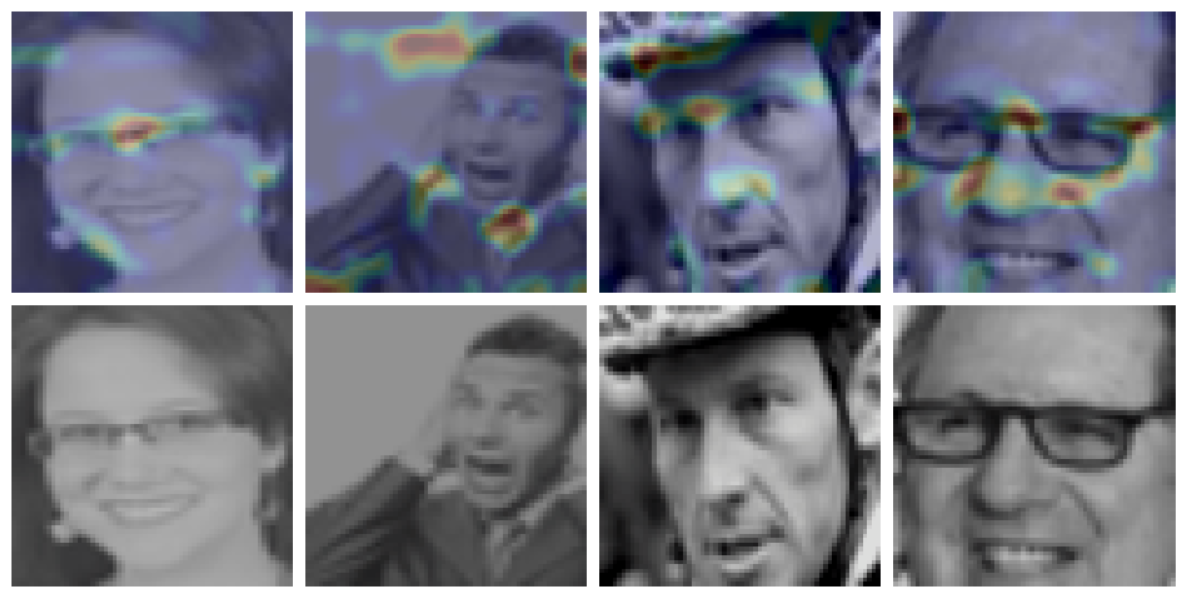
\includegraphics[width=0.8\textwidth]{gradcam_example_faces.png}
    \caption{An example failure case by visualizing the heatmaps of the gradient of a unlabeled SimCLR trained ResNet \citep{chen2020simple} using the GradCAM method \citep{selvaraju2017grad}. The OOD detection task is to detect OOD facial expressions. In this case, the OOD detection method fails as justified by our theoretical work, where the representations do not exhibit a strong gradient in regions commonly associated with facial expressions (i.e., eyebrows, mouth, etc.).}
    \label{fig:grad}
\end{figure}

However, one can unintentionally avoid label blindness problem via the selection of the OOD dataset when constructing OOD benchmarks. Existing methods generally consider ID and OOD data from different datasets, e.g., \citet{fort2021exploring}, \citet{sehwag2021ssd}, and \citet{hendrycks2019using}. In these benchmarks, there is no significant overlap between the ID and OOD input data, allowing OOD detection algorithms to succeed on features independent of the label. To address this issue and to test for label blindness, we introduce the Adjacent OOD detection task to evaluate the performance on OOD detection algorithms when there is significant overlap between the OOD input data and ID input data. We also prove that it is impossible to guarantee that a real world system will never encounter OOD input data that significantly overlaps ID input data.

This work aims to answer the following question: \emph{can we ignore labels when engaging in OOD detection?} Through numerous experiments and theoretical proofs, we show that it is not safe to ignore labels when performing OOD detection. This is contrary to the increasing recent efforts that propose new self supervised, unsupervised, and other unlabeled OOD detection methods. This work's key contributions include:
\begin{itemize}
\item \textbf{The Label Blindness Theorem.} We theoretically prove that any SSL or Unsupervised Learning algorithm will fail when its information required for the surrogate task is independent of the information required for predicting labels. Through this proof, we conclude that there cannot be a generally applicable SSL or Unsupervised learning OOD detection algorithm as there will always exist independent labels due to the no free generalization theorem.

\item \textbf{Adjacent OOD detection benchmarks.} We introduce the concept of bootstrapping without replacement of the ID labels to create the Adjacent OOD detection task. To the authors' knowledge, this OOD detection task is novel to and absent from research in OOD detection. This task evaluates OOD detection when there is significant overlap in OOD data and ID. We also theoretically prove that overlapping OOD and ID data is possible in every real world dataset.

\item \textbf{Impact on existing and future OOD methods.} We demonstrate that existing SSL and Unsupervised Learning OOD methods fail under the conditions suggested by our theory and that existing benchmarks do not capture such failures. We also evaluate zero shot OOD detection methods, which fail in a similar manner to SSL and Unsupervised Learning OOD methods. We make recommendations on the development and testing of future OOD methods.
\end{itemize}

\section{Preliminaries}

\subsection{Labeled and Unlabeled Out-of-Distribution Detection}

The task of out-of-distribution detection is to identify a semantic shift in the data \citep{yang2021generalized}. This is determining when no predicted label could match the true label $\vy \notin \sY_{in}$, where $\sY_{in}$ represents the set of in-distribution training labels. In this case, we would consider the semantic space of the sample and the training distribution to be different, representing a semantic shift. We can express the probability that a sample is out-of-distribution via $P(\vy \notin \sY_{in} | \vx)$. One baseline method to calculate $P(\vy \notin \sY_{in} | \vx)$ is to take $1 - \texttt{MSP}(\vx)$, where $\texttt{MSP}$ is the maximum softmax probability from a classifier for a particular datapoint.

Furthermore, we are only concerned with labels that can be generated using only $\vx$, via function $f$ which depends solely on $\vx$ and no other information. $f$ may represent human labelers that generate $\vy$. If we consider $\sY_{all}$ as the set of all possible labels that can be generated from $f(\vx \in \sX_{all})$, a subset of $\sX_{all}$ considered as $\sX_{training}$ may not contain all labels in $\sY_{all}$. For real world datasets, it is possible that $\sY_{in} \subsetneq \sY_{all}$.

We can also approach the problem of OOD detection without the use of labels. One can train a model on ID data using a surrogate task for the purposes of computing a metric. For example, \citet{sehwag2021ssd} trains a resnet with SimCLR and computes the Mahalanobis distance between the training representations and the test sample representations to compute the OOD score. Alternatively, one could utilize a pretrained model with broad knowledge to compute a metric to use as the OOD score, such as in \citet{wang2023clipn}.

\subsection{Self-Supervised and Unsupervised Learning}

This section covers representation learning and its implications for SSL and unsupervised learning. If there is no mutual information between two random variables, neither can be used to reduce uncertainty about the other \citep{shannon1948mathematical}. In both self-supervised and unsupervised OOD detection, if there is no mutual information between the intermediate representations and the OOD detection task, the OOD detection system cannot reduce uncertainty with respect to the OOD detection task using the intermediate representations.

Representation learning can be formulated as finding a distribution $p(\rvz|\rvx)$ that maps the observations from $\vx \in \sX$ to $\vz \in \sZ$, while capturing relevant information for some primary task. When $\rvy$ represents some primary task, we consider only $\rvz$ that is sufficiently discriminative for accomplishing the task $\rvy$. For simplicity, we consider $\rvy$ as a classification label, but $\rvy$ can represent any objective or task. \citet{federici2020learning} show that this sufficiency is met when the information relevant for predicting $\rvy$ is unchanged when encoding $\rvx \rightarrow \rvz$.

\begin{definition}
    Sufficiency: A representation $\rvz \text { of } \rvx$ is sufficient for $\rvy$ if and only if $I(\rvx ; \rvy \mid \rvz)=0 $.
    \label{definesuff}
\end{definition}

Since there exists the sufficient statistic $\rvx=\rvz$, we must consider the minimal sufficient statistic which conveys only relevant information for predicting $\rvy$. An SSL algorithm seeks to learn the minimal sufficient statistic via the information bottleneck framework \citep{shwartz2023compress}.

\begin{definition}
Minimal Sufficient Statistic. A sufficient statistic $\rvz$ is minimal if, for any other sufficient statistic $\rvs$, there exists a function $f$ such that $\rvz = f(\rvs)$.
\label{defineminsuff}
\end{definition}

Information bottleneck optimization can be expressed as the minimization of the representation's complexity via $I(\rvx;\rvz)$ and maximizing its utility $I(\rvz;\rvy)$. This results in the information theoretic loss function below, where $\beta$ is a trade-off between complexity and utility \citep{shwartz2023compress}. In practice, learning $\rvz$ without $\rvy$ requires a surrogate task $\rvy_{s}$, e.g., \citet{chen2020simple}, with the loss defined as:
\begin{align}
\mathcal{L}=I(\rvx ; \rvz)-\beta I(\rvz ;\rvy).
\end{align}
It should be noted that the primary task $\rvy$ may be equal to the SSL task $\rvy_{s}$. In such a case, compression towards the minimal sufficient statistic still occurs. This is important because unsupervised methods for deep neural networks (DNNs) will use a surrogate task $\rvy_{u}$ to train the DNN's weights. Thus, if we assign the primary task for an unsupervised learning method to be equal to its surrogate task, it will behave identically to SSL from the perspective of information theory.

When $\rvx$ has higher information content than $\rvy$, there exists information in $\rvx$ that is not relevant for predicting $\rvy$. This can be better understood by dividing $I(\rvx;\rvz)$ into two terms \citep{federici2020learning} as follows:
\begin{align}
I(\rvx ; \rvz)=\underbrace{I(\rvx ;\rvz \mid \rvy)}_{\text {superfluous information }}+\underbrace{I(\rvz ; \rvy)}_{\text {predictive information }}. \label{superfluous}
\end{align}

However, superfluous information is not affected by the labels of primary task, only by $\rvx$ and $\rvy_{s}$. Using information theory, we can show that any SSL OOD detection algorithm will fail when the surrogate task $\rvy_{s}$ is independent of the labels in the in-distribution dataset. This applies to unsupervised OOD detection algorithms that also use a surrogate task.

\section{Guaranteed OOD Detection Failure}

This section introduces the concept of \textbf{Label Blindness}, with one key supporting theorem and one key supporting lemma. Note that $R_{\rvx}$ represents the support of random variable $\rvx$ such that $R_{\rvx} = \{\vx \in \R : P(\vx) > 0\}$. For clarity, we refer to cases where $I(\rvx_1; \rvx_2) = 0$ as \textbf{Strict Label Blindness} and discuss \textbf{Approximate Label Blindness} $I(\rvx_1; \rvx_2) \approx 0$ later in this section.

\subsection{Label Blindness Theorem (Strict Label Blindness)}

We identify a guarantee of OOD detection failure for any information bottleneck-based optimization process if the unlabeled learning objective is independent from labels used to determine the ID set, described by Corollary \ref{mainbodyfailood}. This corollary is derived from two concepts: strict label blindness in the minimal sufficient statistic and the independence of filtered distributions. We first consider the minimal sufficient statistic and how it leads to strict label blindness; see Theorem \ref{mainbodygenloss}.

\begin{theorem}[Strict Label Blindness in the Minimal Sufficient Statistic]
    Let $\rvx$ come from a distribution. $\rvx$ is composed of two independent variables $\rvx_1$ and $\rvx_2$. Let $\rvy_1$ be a surrogate task such that $H(\rvy_1|\rvx_1) = 0$. Let $\rvz$ be any sufficient representation of $\rvx$ for $\rvy_1$ that satisfies the sufficiency definition \ref{definesuff} and minimizes the loss function $\mathcal{L} = I(\rvx_1 \rvx_2; \rvz) - \beta I(\rvz;\rvy_1)$. The possible $\rvz$ that minimizes $\mathcal{L}$ and is sufficient must meet the condition $I(\rvx_2; \rvz) = 0$.
    \label{mainbodygenloss}
\end{theorem}

\textit{Proof:} See Appendix \ref{app:genloss} for the complete proof.

Intuitively, the minimal sufficient representation cannot encode any information independent of the surrogate learning objective, otherwise it would not be minimal. This means that the representation will be blind to any label built upon the independent information.

However, Theorem \ref{mainbodygenloss} is not sufficient to guarantee OOD failure. This is because the selection of the ID training set could change the learned representation $\rvz$, possibly improving OOD detection performance by increasing mutual information, $I(\rvx_2;\rvz) > 0$. We formally disprove this possibility through Lemma \ref{mainbodyfilter}.

\begin{lemma}[Independence of Filtered Distributions]
    Let $\rvx$ come from a distribution. $\rvx$ is composed of two independent variables $\rvx_1$ and $\rvx_2$. For $\rvx_2'$ where $R_{\vx_2'} \subset R_{\vx_2}$, there exists no $\rvx_2'$ such that $H(\rvx_1|\rvx_2') < H(\rvx_1)$.
    \label{mainbodyfilter}
\end{lemma}

\textit{Proof:} See Appendix \ref{app:filter} for the complete proof.

Lemma \ref{mainbodyfilter} states that filtering on a label generated on one of two independent variables cannot provide information about the other. This applies to the selection of ID data from the population, if the selection criteria is independent of the learning objective. This means that the strict label blindness properties predicted by Theorem \ref{mainbodygenloss} will apply to ID training data. These two concepts bring us to our main result -- strict label blindness in filtered distributions; see Corollary \ref{mainbodyfailood}.

\begin{corollary}[Strict Label Blindness in Filtered Distributions]
    Let $\rvx$ come from a distribution. $\rvx$ is composed of two independent variables $\rvx_1$ and $\rvx_2$. Let $\rvy_1$ be a surrogate task such generated by $\vy_1 = f_1(\vx_1)$ $H(\rvy_1|\rvx_1) = 0$. Let $\rvy_2$ be a label such that $H(\rvy_2|\rvx_2) = 0$ and $\vy_2 = f_2(\vx_2)$. Let $\sY_{in}$ be as subset of labels $\sY_{in} \subset R_{\rvy_2}$. Let $\rvx'$ be a subset of $\rvx$ where $R_{\rvx'} = R_{\rvx} \cap \{\vx \in \R: f_2(\vx_2) \in \sY_{in} \}$ such that $\rvx'$ is composed of independent variables $\rvx_1'$ and $\rvx_2'$ and $\vy_1' = f_1(\vx_1')$. The sufficient representation $\rvz$ learned by minimizing $\mathcal{L} = I(\rvx_1' \rvx_2'; \rvz) - \beta I(\rvz;\rvy_1')$ must have $I(\rvx_2;\rvz) = 0$ and $I(\rvy_2;\rvz) = 0$.
    \label{mainbodyfailood}
\end{corollary}

\textit{Proof:} See Appendix \ref{app:failood} for the complete proof.

This means that, when we select the ID training data, if the selection criteria and labels are independent of the surrogate learning objective, then we can guarantee failure in OOD detection due to the absence of any information in the learned representation $\rvz$. For simplicity, we refer to this concept, supported by Corollary \ref{mainbodyfailood}, as the problem of \textbf{Strict Label Blindness}.

In summary, when the surrogate learning task can be achieved without learning about features relevant for the label, it will not learn any features relevant for the label. If the SSL or unsupervised learning method fails to learn any label-relevant features, then any OOD detection algorithm built from those representations cannot differentiate between the labels selected as ID and those not selected as ID. This guarantees failure in OOD detection because no label information passes through the information bottleneck.

\subsection{Implications of Strict Label Blindness in Real World Situations}

We can utilize Fano Inequality to extend our understanding of strict label blindness to consider situations where the variables are not fully independent. The lower bound for prediction error is defined by the entropy of the target label $\rvy$ less the mutual information between the input $\rvx$ and target label, as shown in Theorem \ref{fano}. Under strict label blindness, when $I(\rvx;\rvy) = 0$, the lower bound for error is at its maximum. When $I(\rvx;\rvy) \approx 0$, the lower bound for error is large enough to be unreliable. We refer to this condition as \textbf{Approximate Label Blindness} and we conduct experiments to evaluate this condition. Unless specified as strict, label blindness refers to the approximate case.

\begin{theorem}[Fano's Inequality]
Let $\rvy$ be a discrete random variable representing the true label with $\mathcal{Y}$ possible values and cardinality of $|\mathcal{Y}|$ and $\rvx$ be a random variable used to predict $\rvy$. Let $e$ be the occurrence of an error such that $\rvy \neq \hat{\rvy}$ where $\hat{\rvy} = f(\rvx)$. Let $H_b$ represent the binary entropy function such that $H_b(e)=-P(e) \log P(e)-(1-P(e)) \log (1-P(e))$. The lower bound for $P(e)$ increases with lower $I(\rvx;\rvy)$.
\begin{align}
H_b(e) + P(e) \log(| \mathcal{Y} |-1) \geq H(\rvy) - I(\rvx; \rvy).
\end{align}
\label{fano}
\end{theorem}

\subsection{Theoretical Implications}

Our work applies to deep neural networks (DNNs) trained without labels for the purpose of OOD detection. The key assumption of information bottleneck compression is generally applicable to DNNs \citep{shwartz2017opening}. Regardless of other assumptions, such as the multi-view assumption, an information bottleneck DNN trained without labels will still compress data irrelevant to its loss objective, even if that data is relevant for its intended task. It does not matter what task the training process was originally designed for because the unlabeled training process ultimately generates/adheres to its own learning objective. For any learning objective, there will exist an independent feature unless compression is not possible, as in $I(\rvx;\rvy) = I(\rvx;\rvx)$. If there is compression, then there exists labels for which OOD detection failure is guaranteed.

Our work predicts a guarantee of failure only when we consider the OOD set of all non-ID data. In our own experiments and in work by \citet{sehwag2021ssd, hendrycks2019using, liu2023unsupervised}, purely self-supervised and unsupervised OOD methods can perform well against common benchmark OOD sets. This suggests that the choice of ID set and OOD set pairs can unintentionally hide label blindness failure. Alternatively, we can also construct a test to identify if the OOD detection algorithm suffers from label blindness. To construct such a test, we rely on the insight from Corollary \ref{mainbodyfailood} and the use of a simple statistical method.

\section{Benchmarking for Label Blindness Failure}

\subsection{Bootstrapping and the Adjacent OOD Benchmark}

One logical consequence of Corollary \ref{mainbodyfailood} is that one cannot avoid failure due to label blindness by selecting different labels for one's ID set, so long as the label selection is independent from the learning objective. To test any OOD detection algorithm for label blindness failure, this simply entails selecting different labels for one's ID set. To construct this benchmark, we randomly sample labels to be considered as ID and other labels to be consider OOD. This is similar to bootstrapping, but without replacement. If an OOD detection algorithm is `approximately label blind', its average OOD detection performance across the samples should be poor. We refer to this as the \textbf{Adjacent OOD Detection Benchmark}.

\subsection{Why Adjacent OOD is Safety-Critical to Almost All Real World Systems}

The Adjacent OOD detection benchmark evaluates the performance of OOD detection algorithms when there may be a significant overlap between the ID data and OOD data. This condition applies to all systems where it is impossible to guarantee that there will be no significant overlap in the feature space between ID and OOD data. This is true for almost all real world systems and is theoretically proven below.

\begin{theorem}[Unavoidable Risk of Overlapping OOD Data]
Let $\rvx$ come from a distribution. Let $f$ be some labeling function to generate labels $\rvy$ such that $\vy = f(\vx)$, where there are at least two unique labels $|R_\rvy| > 1$. Let $\rvx_{in}$ be a random subset of $\rvx$ where $R_{\rvx_{in}} \subsetneq R_\rvx$ and $|R_{\rvx_{in}}| < \infty$. Let $\rvy_{in}$ be labels generated from $\vy_{in} = f(\vx_{in})$. The probability that a randomly selected $\vx$ contains $\vy$ not present in $R_{\rvy_{in}}$ is always greater than 0.
\label{mainbodyoverlap}
\end{theorem}

\textit{Proof:} See Appendix \ref{app:overlaprisk} for the complete proof.

In theory, this risk can be reduced to an acceptable level by adding more data to the training dataset. However, this reduction in risk requires the assumption that the collected data is randomly sampled. This is almost never true for real world datasets and often the opposite is true, where the nature of sampling can significantly increase this risk.

One risk factor present in every real world dataset is the dataset creation date. By creating the dataset at any specific point in time, the dataset cannot be randomly sampled with respect to time because it is impossible to collect data from the future. For example, if one were to create a dataset of diseases today, it would not contain any future diseases. In this example, the probability that the training dataset is incomplete is 100\%, which guarantees that there will be OOD data that significantly overlaps with ID data. For most real world systems, the only safe assumption is that there may be OOD data that overlaps with ID data and it is necessary to plan accordingly.

The failure predicted by the label blindness theory is easiest to detect in the adjacent OOD situation. Where there is a likelihood of adjacent data, Theorem \ref{mainbodyfailood} predicts OOD detection failure. Where there is no adjacent data, features independent of the label can still be used to distinguish between ID data and non adjacent OOD data, as shown in various experiments in this paper and others \citep{sehwag2021ssd, hendrycks2019using, liu2023unsupervised}.

\subsection{Comparing Adjacent, Near, and Far OOD Benchmarks}

Many unlabeled OOD methods generally perform quite well on far and near OOD tasks. Far OOD is often defined by ID and OOD sets with different semantic labels and styles \citep{fang2022out}. One such far OOD benchmark is MNIST as ID data and CIFAR10 as OOD data. Near OOD contains ID and OOD sets with similar semantic labels and styles \citep{fang2022out}. These tasks tend to be more difficult for existing OOD detection methods than far OOD detection tasks. One such near OOD benchmark is CIFAR10 as ID and CIFAR100 as OOD. However, the overlap in the near OOD detection benchmarks is significantly less than the adjacent OOD detection benchmark, which evaluates the maximum possible feature overlap. For example, an Adjacent OOD benchmark on the ICML Facial Expressions dataset may contain the same face with different expressions, resulting in significant feature overlap. These existing benchmarks do not provide sufficient safety guarantees in applications where there may be significant overlap between ID and OOD data.

\subsection{Implications for OOD from Unlabeled Data}

While methods that utilize only unlabeled data, such as \citet{sehwag2021ssd, liu2023unsupervised, guille2024cadet}, show promising results on both near and far OOD tasks, their performance in the adjacent OOD detection tasks depends on the mutual information between the learned representation and the ID labels. Our theoretical work suggests that such methods will perform poorly, if the surrogate task is independent of the labels.

The adjacent OOD detection benchmark can also evaluate the performance of zero shot OOD detection methods. While our theoretical work does not extend to pretraining due to the use of labels, it is also still important to consider the performance when OOD data overlaps ID data.

\section{Experimental Results}

We conduct the following experiments to verify the existence of label blindness in unlabeled OOD detection methods. All hyperparameters and configurations were the best performing from their respective original paper implementations, unless noted otherwise. Experiments are repeated 3 times.

\subsection{Experimental Setup}

\paragraph{Supervised Baseline.}
We use Maximum Softmax Probability (MSP) \citep{hendrycks2016baseline} as our baseline supervised method for comparison. We augment the training data using random rotation, horizontal flip, random crop, gray scale, and color jitter. Images are resized to $64\times64$. We train using stochastic gradient descent with momentum and a cosine annealing learning schedule. We train for $10$ warm up epochs followed by $150$ regular epochs, selecting the weights with the highest validation accuracy. We use a standard ResNet50 architecture.

\paragraph{Self-supervised Baselines.}
We use two SSL methods to evaluate how representations are learned, SimCLR \citep{chen2020simple} and Rotation Loss (RotLoss) \citep{hendrycks2019using}. Images are resized to $64\times64$ for both cases. For SimCLR, we augment the training data using random rotation, horizontal flip, random crop, gray scale, and color jitter. For Rotation Loss, we use only random crop and horizontal flip. We train using stochastic gradient descent with momentum (and a cosine annealing learning schedule) and employ a standard ResNet50 architecture and train for $10$ warm up epochs followed by $500$ regular epochs, selecting the weights with the best-learned representations. We use a KNN classifier to determine the best representations during validation at the end of each epoch.

To evaluate OOD performance, we use two methods to generate the OOD score of each sample, SSD \citep{sehwag2021ssd} and KNN, similar to \citet{sun2022out}. SSD considers the OOD score as the Mahalanobis distance of the sample from the center of all in-distribution training data samples. The KNN method considers the OOD score as the Euclidean distance from the $N$th nearest neighbor of the test sample to all in-distribution training samples. Both methods are distance based OOD detection and are commonly used with representation learning. We use the same representation mentioned in the previous paragraph.

\paragraph{Unsupervised Baseline.}
To consider how an unsupervised OOD detection method functions, we evaluate the diffusion impainting OOD detection method proposed by \citet{liu2023unsupervised} using code provided in their paper's linked repository. We utilize the training configuration that generated the paper's main results, which involved an alternating checkerboard mask 8 × 8, an LPIPS distance metric to calculate the OOD score, and 10 reconstructions per image. We modify only the input image size to be $64\times64$ for all datasets and run additional experiments to evaluate performance on their alternative MSE distance metric. This method is representative of other generative methods, such as \citet{xiao2020likelihood}.

\paragraph{Zero-shot Baseline.}
To consider how well zero shot learning algorithms perform, we evaluate the CLIPN model presented by \citet{wang2023clipn}. We utilize their pretrained weights provided in their paper's repository and perform zero shot OOD detection on our adjacent OOD detection benchmark. We evaluate CLIPNs performance using 3 of their paper's algorithms, Maximum Softmax Probability, Compete to Win (CTW), and Agree to Differ (ATD).

\subsection{Adjacent OOD Datasets}

To create the Adjacent OOD detection task, we randomly split $25$\% of all classes into the OOD set and retain $75$\% as the ID set. We also repeat our experiments three times with different seeds to account for different splits of the ID and OOD set. Only ICML Facial expressions has a major class imbalance for one of its seven classes.

The ICML Facial Expressions dataset \citep{icmlface} contains seven facial expressions split across $28,709$ faces in the train set and $7,178$ in the test set. The expressions include anger, disgust, fear, happiness, sadness, surprise, and neutral. Self-supervised algorithms may not learn relevant features for distinguishing expressions and instead learn features relevant for distinguishing faces.

The Stanford Cars dataset \citep{KrauseStarkDengFei-Fei_3DRR2013} contains $16,185$ images taken from $196$ classes of cars. The data is split into $8,144$ training images and $8,041$ testing images, with each class being split roughly $50$-$50$. Classes are typically very fine-grained, at the level of Make, Model, Year, e.g., 2012 Tesla Model S or 2012 BMW M3 coupe. This creates a particularly challenging Adjacent OOD task because of the reliance on more subtle features to differentiate cars.

The Food 101 dataset by \citet{bossard14} consists of $101$ food categories and $101,000$ images. There are $250$ manually reviewed test images and $750$ training images for each class. Note that training images were not cleaned to the same standard as the test images and will contain some mislabeled samples. We believe that this should not significantly detract from the Adjacent OOD nature of the dataset.

\subsection{Experimental Results}

Experimental results for Adjacent OOD are presented in Table \ref{tab:results}. It is apparent that the baseline supervised method performs better than most unlabeled methods on the Adjacent OOD detection task. In cases where the unlabeled methods exhibits performance as good as random guessing, it is likely that the learned representation contains little information about the semantic label. This is contrary to the reported performance improvements presented in unlabeled OOD papers \citep{sehwag2021ssd, hendrycks2019using, liu2023unsupervised}, as our experimental results suggest unlabeled OOD is significantly worse than a simple MSP baseline.

It is important to note that the zero shot CLIPN method performs well when the label text's usage in pretraining is similar to the label text's usage in the ID data. In the case of the Cars dataset, the pretraining dataset CC3M \citep{sharma2018conceptual} contains many images captioned with the make and model of various cars, resulting in good performance. The Food dataset also sees similar label usage in the pretraining set. However, the Faces dataset's labels are not aligned. For example, there are multiple images associated with the emotion angry that do not contain a human face, such as an image of a angry fist. When there is little or no mutual information between the pretraining data and the ID labels, zero shot methods will perform poorly in OOD detection tasks.

\begin{table}[h]
\caption{Results from experiments across various datasets and methods. Unlabeled methods perform poorly in adjacent OOD detection. CLIPN performance is due to labels present in the pretraining dataset. Higher AUROC and lower FPR is better.}
\vspace{2mm}
\centering
\begin{tabular}{l|ll|ll|ll}
\toprule
                & Faces    &          & Cars     &           & Food     &          \\ \hline
Method          & AUROC    & FPR95    & AUROC    & FPR95     & AUROC    & FPR95    \\ \midrule
Supervised MSP  & 70.8±0.3 & 88.2±0.2 & 69.2±0.9 & 88.8±0.8  & 78.8±1.2 & 81.1±1.6 \\ \midrule
SimCLR KNN      & 52.0±4.2 & 95.0±1.3 & 52.5±0.4 & 94.0±0.5  & 61.1±2.8 & 91.6±1.6 \\
SimCLR SSD      & 55.0±4.5 & 95.1±2.0 & 52.7±0.7 & 93.7±1.1  & 64.4±0.8 & 89.3±0.5 \\
RotLoss KNN     & 46.1±2.5 & 95.8±0.4 & 51.1±0.6 & 94.8±0.7  & 49.7±3.8 & 94.9±0.9 \\
RotLoss SSD     & 46.6±3.0 & 95.7±0.5 & 50.7±1.9 & 95.0±1.2  & 50.7±3.6 & 94.9±0.9 \\ \midrule
Diffusion LPIPS & 54.7±4.6 & 94.2±3.7 & 53.8±1.8 & 93.9±1.2  & 52.9±2.2 & 94.4±0.6 \\
Diffusion MSE   & 55.3±2.2 & 94.2±1.4 & 51.6±1.6 & 94.4±0.5  & 52.5±3.4 & 94.2±0.6 \\ \midrule
CLIPN CTW       & 47.0±1.4   & 97.3±0.3 & 65.0±5.1   & 69.4±9.4  & 70.9±2.9 & 69.1±7.0   \\
CLIPN ATD       & 44.2±1.4 & 97.5±0.2 & 81.1±4.3 & 56.6±10.4 & 84.9±0.2 & 53.9±4.5 \\
CLIPN MSP       & 58.7±4.4 & 95.9±1.4 & 76.5±1.4 & 75.4±0.6  & 80.5±1.6 & 74.0±1.4   \\ \bottomrule
\end{tabular}
\label{tab:results}
\end{table}

We observe decent OOD performance on the unlabeled SimCLR compared to the labeled supervised MSP for CIFAR10 and CIFAR100 datasets. This is likely because the SimCLR algorithm is better at learning the relevant features in these datasets and that the classes are more visually dissimilar, resulting in less overlap of OOD and ID data. We also show strong results for far OOD performance for SimCLR based OOD detection, which confirms findings in papers that test unlabeled OOD methods against a far OOD detection benchmark \citep{sehwag2021ssd, tack2020csi, liu2023unsupervised, guille2024cadet, wang2023clipn}.

\section{Discussion}

\subsection{Impact of Label Blindness on Future Research}

A consequence of the label blindness theorem is that there cannot exist a single unlabeled OOD detection algorithm for all unlabeled data. However, unlabeled learning methods, such as SimCLR, are vital for improving OOD detection. The model of \citet{sun2022out} learns representations using a supervised version of SimCLR, similar to \citet{khosla2020supervised}. The combination of a multi-view information bottleneck with supervised classes produces a more robust representation of the in-distribution data than using only a supervised loss. Recent work by \citet{du2024does} provides a strong theoretical basis for why unlabeled data can improve OOD detection performance.

The Adjacent OOD detection benchmark addresses a critical safety gap in existing OOD detection research. Current benchmarks often use datasets with minimal feature overlap between ID and OOD data, which can mask the label blindness problem. In real-world applications, especially safety-critical ones, it is essential to evaluate OOD detection methods under conditions where ID and OOD data may have significant feature overlap.

Our findings suggest that practitioners should be cautious when deploying unlabeled OOD detection methods in scenarios where the training data may not capture all relevant semantic variations. The theoretical guarantees provided by our label blindness analysis indicate that such methods may fail catastrophically when encountering OOD data that shares features with ID data but differs in the semantic labels.

\subsection{Recommendations for Future OOD Detection Research}

Based on our theoretical and empirical findings, we recommend several directions for future research:

\begin{itemize}
\item \textbf{Hybrid approaches}: Combining supervised and self-supervised learning objectives may help mitigate label blindness by ensuring that label-relevant features are preserved during representation learning.

\item \textbf{Adjacent OOD evaluation}: All OOD detection methods should be evaluated on Adjacent OOD benchmarks to assess their robustness to scenarios with high feature overlap between ID and OOD data.

\item \textbf{Information-theoretic analysis}: Future unlabeled OOD detection methods should include theoretical analysis of the mutual information between their learning objectives and the target labels to identify potential label blindness issues.

\item \textbf{Domain-aware methods}: Developing methods that can explicitly model and account for domain-specific features may help address some of the limitations identified in our work.
\end{itemize}

\section{Conclusion}

In this work we provide an answer to the question, can we ignore labels for OOD detection? Our theoretical work shows that the answer is no, unless the unlabeled method happens to capture the relevant features and does not need to work for different sets of labels. Due to the lack of existing benchmarks that capture the theoretically expected failure, we introduce a novel type of OOD task, Adjacent OOD detection. This task addresses the critical safety gap caused by significant overlap of ID and OOD data. We show that the Adjacent OOD task accurately captures the failure in unlabeled OOD detection that is hypothesized by our theory.

The label blindness theorem demonstrates that when the surrogate learning task used in self-supervised or unsupervised learning is independent of the features relevant for label prediction, OOD detection is guaranteed to fail. This fundamental limitation cannot be overcome by simply selecting different ID datasets, as the independence property is preserved under filtering operations.

Our experimental results confirm the theoretical predictions, showing that unlabeled OOD detection methods perform poorly on Adjacent OOD benchmarks where there is significant feature overlap between ID and OOD data. In contrast, these same methods often perform well on traditional far OOD benchmarks, highlighting the importance of comprehensive evaluation.

The Adjacent OOD detection benchmark introduced in this work provides a crucial tool for evaluating the robustness of OOD detection methods in realistic scenarios. This benchmark addresses a previously ignored safety gap in OOD detection research and should be adopted as a standard evaluation protocol for future work.

We hope our work will help support more robust research into OOD detection and improve the safety of AI applications. The theoretical framework and empirical findings presented here provide important guidance for developing more reliable OOD detection methods that can handle the complexities of real-world deployment scenarios.





\chapter{Domain Feature Collapse in Single-Domain OOD Detection}

\textit{This chapter is based on work submitted to AAAI 2026: "Domain Feature Collapse: Implications for Out-of-Distribution Detection and Solutions" by Hong Yang, Qi Yu, and Travis Desell.}

\section{Introduction}

The deployment of deep neural networks (DNNs) in safety-critical domains -- such as autonomous driving \citep{ramanagopal2018failing}, biometric authentication \citep{wang2021deep}, and medical diagnostics \citep{bakator2018deep} -- has spurred growing interest in ensuring their reliability. In these contexts, the traditional closed-world assumption \citep{krizhevsky2012imagenet}, where training and test data are drawn i.i.d. from the same in-distribution (ID), is no longer valid. Instead, models must operate under open-world conditions \citep{drummond2006open}, where inputs encountered at test time may stem from entirely different, out-of-distribution (OOD) sources.

Many state-of-the-art OOD detection methods demonstrate strong performance across established benchmarks \citep{zhang2023openood}. However, these benchmarks almost exclusively use in-distribution sets that contain samples and classes from a wide variety of domains, such as CIFAR10/100 \citep{cifar10} and ImageNet \citep{deng2009imagenet}. While this approach provides a broad testbed for evaluating OOD robustness, it implicitly biases models and methods toward handling multi-domain in-distribution settings. As a result, there exists a gap in the literature: current OOD detection techniques are largely tailored to scenarios where the ID data is inherently diverse, rather than narrow or homogeneous.

The single domain setting is understudied in bleeding edge OOD detection research, yet it has been heavily studied in the application of OOD methods for downstream tasks. Single-domain OOD detection is particularly important in application areas such as medical imaging \citep{zhang2021out}, satellite imagery \citep{ekim2024distribution}, and agriculture \citep{saadati2024out}, where models are often deployed in narrowly scoped environments with highly consistent data characteristics.

This chapter introduces the concept of and theoretically proves the existence of \textbf{domain feature collapse}. Through information theory and bottleneck compression, we show that artificial neural networks will remove domain specific features from their learned representations, under the single domain setting. This leads to a situation where OOD detection relies solely on class-specific features, while ignoring domain-specific features. Unfortunately, this failure results in higher OOD detection error rates when the ID set is single domain versus multi-domain.

\section{Problem Formulation}

\subsection{Single-Domain Datasets and Domain Features}

We define the dataset's domain $\rvd$ as a value generated from some domain labeling function $f_{\rvd}(\rvx)$. For the purposes of this work, we are primarily concerned with cases where the data comes from a single domain $\rvd_1$, such that $\forall \rvx \in  \{f_{\rvy}(\rvx) \in  \sY_{in}\}, f_{\rvd}(\rvx) = \rvd_1$. In these situations, we can conclude that $\forall \rvx \in \{f_{\rvd}(\rvx) \neq \rvd_1\}, f_{\rvy}(\rvx) \notin \sY_{in}$, since any data outside of the domain cannot possibly have an in-distribution label.

For this work, we define domain features $\rvx_\rvd$ such that they do not overlap with class features $\rvx_\rvy$, implying $I(\rvx_\rvd:\rvx_\rvy) = 0$. The independence of domain and class features only applies to the training set, as domain features would provide useful information in the context of $\sX_{all}$. Note that this also implies that $\neg(\forall\rvx,  f_\rvy(\rvx_\rvy) = f_\rvy(\rvx))$ and $\forall\rvx, f_\rvy(\rvx_\rvy, \rvx_\rvd) = f_\rvy(\rvx)$. For both domain and class features, we refer to the minimal set of features, as per the minimal sufficient statistic definition.

Examples of single domain datasets could include a medical chest X-ray dataset \citep{yang2023medmnist}, a geology dataset \citep{rock_data}, or a satellite imagery dataset \citep{helber2019eurosat}. Further note that domains exist in a hierarchy; for instance, the domain of cats is a subdomain of mammals which is itself a subdomain of animals. This means that there is a domain that includes all things, but such a domain would have $\{\rvx_\rvd\} = \emptyset$. For a wide domain with a wide variety of classes, we expect fewer domain features and more class features.

There exist datasets that could be labeled as a single domain $\rvd_1$ yet contain $|\{\rvx_\rvd\}| \approx 0$. For example, if one were to treat ImageNet as a single domain, the set of domain features that do not overlap with class features is likely to be zero or nearly zero. We refer to such datasets as multi-domain datasets, as their diversity of classes require multiple domains.

\section{Theoretical Analysis: Domain Feature Collapse}

This section theoretically proves that any supervised model under a label-based training objective will learn a representation that contains no information on domain features, such that $I(\rvx_\rvd, \rvz) = 0$, if full bottleneck compression occurs. This is considered to be strict domain feature collapse and relies on full information bottleneck compression:

\begin{theorem}[Strict Domain Feature Collapse in the Minimal Sufficient Statistic]
Let $\rvx$ come from a distribution. $\rvx$ is composed of two independent variables $\rvx_\rvd$ and $\rvx_\rvy$, where $\rvx_\rvd$ is a set of domain features as per Definition \ref{def:domainfeatures}. Let $\rvd$ be a domain label generated from $f_\rvd(\rvx_\rvd) = \rvd_1$, where $\rvd_1$ is a constant value for all $\rvx$. Let $\rvy$ be a class label generated from $f_\rvy(\rvx_\rvd, \rvx_\rvy) = \rvy$. Let $\rvz$ be any sufficient representation of $\rvx$ for $\rvy$ that satisfies the sufficiency definition and minimizes the loss function $\mathcal{L} = I(\rvx_\rvd \rvx_\rvy; \rvz) - \beta I(\rvz;\rvy)$. The possible $\rvz$ that minimizes $\mathcal{L}$ and is sufficient must meet the condition $I(\rvx_\rvd; \rvz) = 0$.
\label{thm:domainfeaturecollapse}
\end{theorem}

\begin{proof}
The proof follows from the information bottleneck principle and the independence of domain and class features in single-domain settings. Since $\rvx_\rvd$ and $\rvx_\rvy$ are independent ($I(\rvx_\rvd:\rvx_\rvy) = 0$) and the domain label $\rvd$ is constant for all training samples, the domain features $\rvx_\rvd$ provide no information about the class label $\rvy$ within the training distribution.

Under the information bottleneck objective, the representation $\rvz$ seeks to minimize $I(\rvx; \rvz)$ while maximizing $I(\rvz; \rvy)$. Since $I(\rvx_\rvd; \rvy) = 0$ in the training distribution, including domain features in $\rvz$ would increase the complexity term $I(\rvx; \rvz)$ without contributing to the utility term $I(\rvz; \rvy)$. Therefore, the optimal representation under bottleneck compression will satisfy $I(\rvx_\rvd; \rvz) = 0$.
\end{proof}

Intuitively, the minimal sufficient representation cannot encode any information independent of the learning objective, otherwise it would not be minimal. Due to the definition of $\rvx_\rvd$ as domain features independent of class features, it is clear that compression results in the loss of domain features in the learned representation. This is contrary to the desired outcome, which is to learn $\hat{\rvy} = g(\rvx_\rvd, \rvx_\rvy)$, as this would match the labeling function $\rvy = f_\rvy(\rvx_\rvd, \rvx_\rvy)$. Instead, the model learns $\hat{\rvy} = g(\rvx_\rvy)$ because the domain features $\rvx_\rvd$ are not predictive of the class in the context of the training data.

The lack of domain features is not problematic for safety purposes when $\forall \rvx \in \sX_{all}, H(\rvd|\rvx_\rvy) = 0$; it is safe when all out-of-domain data points contain no in-distribution class features. However, this is difficult to guarantee in an open world setting, as we do not possess information on the OOD distribution. For example, a model might learn that a Tyrannosaurus rex is a dinosaur that stands on two feet and proceed to classify ``Barney'' (a purple dinosaur character from a children's TV show) as a dinosaur, ignoring the fact that it is purple.

\subsection{Implications for OOD Detection}

Domain feature collapse creates a critical safety gap in OOD detection. When a model trained on single-domain data encounters out-of-domain samples that contain in-distribution class features, it may confidently misclassify them because it cannot recognize the domain shift. This is particularly dangerous in safety-critical applications where the cost of false negatives (failing to detect OOD samples) is high.

The problem is exacerbated by model overfitting, where a model may learn only a subset of $\rvx_\rvy$ as opposed to the full set of features intended by the practitioner. Suppose we have a bird dataset made up of blue jays and cardinals. A model may only learn that blue jays are blue and assume that any blue object is a blue jay. Such a model would be safer if it could determine the domain of the blue object as a bird, before assuming it is a blue jay.

It should also be noted that full information bottleneck compression may not occur in real world scenarios, yet we can expect that some level of compression would still occur. In such cases, we can use Fano's Inequality to extend our theory of strict domain feature collapse onto partial compression cases. By Fano's Inequality, we would expect to observe unsafe and unreliable OOD detection conditions even with small $I(\rvx_\rvd; \rvz)$.

\section{Domain Filtering: A Solution to Domain Feature Collapse}

To address the risk of domain feature collapse in supervised networks, we propose a two-stage process that explicitly accounts for domain information before applying traditional OOD detection methods.

\subsection{Two-Stage Detector: Domain Filtering + OOD Detection}

The proposed solution utilizes a two-stage process. In the first stage, a pretrained network is used to determine if a data sample is in-domain. In the second stage, an OOD detector is used to determine if in-domain samples are also in-distribution. This requires the assumption that there exists no in-distribution data sample that is out-of-domain, which is consistent with our earlier definitions.

We evaluate a K-nearest neighbors (KNN)-based domain filter, similar to a KNN-based OOD detector proposed by \citet{sun2022out}. To calibrate the domain filter, we calculate the domain threshold $\rvt_\rvd$ such that $P(f_{knn}(\{\rvx \in \sX_{train}\}) \leq \rvt_\rvd) = p$, where $f_{knn}$ is a KNN function considering the $k$th neighbor and $p$ is a hyper parameter set to $p = 0.99$. Essentially, we select a distance such that 99\% of the training data falls within that distance. The two stage process considers all samples with $f_{knn} > \rvt_d$ as OOD (due to it being out-of-domain) and uses the second stage detector to determine an OOD score for samples with $f_{knn} \leq \rvt_d$.

\begin{algorithm}
\caption{Two-Stage Domain Filtering for OOD Detection}
\label{alg:domainfiltering}
\begin{algorithmic}[1]
\Require Training set $\sX_{train}$, test sample $\rvx$, domain threshold $\rvt_\rvd$, OOD detector $f_{OOD}$
\State Compute $d_{knn} = f_{knn}(\rvx, \sX_{train})$ \Comment{KNN distance to training data}
\If{$d_{knn} > \rvt_\rvd$}
    \State \Return OOD (out-of-domain)
\Else
    \State \Return $f_{OOD}(\rvx)$ \Comment{Apply second-stage OOD detector}
\EndIf
\end{algorithmic}
\end{algorithm}

This process ensures that only a small percentage (1\%) of in-domain samples will be flagged as false positives in the first stage. While there are alternative distance calculation methods and percentile thresholds available, we find that a KNN filter at the 99th percentile with $K = 50$ works well as a first stage domain filter.

\subsection{Relationship to Near, Far, and Adjacent OOD}

In most recent work, such as \citet{fort2021exploring}, and in the OpenOOD framework \citep{yang2022openood, zhang2023openood}, there is a distinction between near and far OOD. Near OOD refers to out-of-distribution samples that are semantically different from the training data but visually or structurally similar. Far OOD refers to samples that are both semantically and visually dissimilar, often coming from completely unrelated domains.

However, by definition, both near and far OOD must be considered out-of-domain when the training data comes from a single domain. If an in-distribution dataset is composed of a single domain, e.g., X-rays, where $\{\rvx_\rvd\} \neq \emptyset$, existing near and far OOD benchmarks will be considered out-of-domain, as they would not be considered in the same domain by $f_\rvd$. We observe that the domain filter is very capable at detecting both near and far OOD benchmark datasets as out-of-domain.

This is in contrast to the adjacent OOD benchmark \citep{yangcan}, which explicitly tests OOD detection performance on in domain samples that are out-of-distribution. The adjacent OOD benchmark constructs a new in-distribution set using a random subset of the training set classes. It then evaluates the OOD performance against the remaining training set classes as if they were OOD, allowing us to consider the impact of in-domain yet OOD samples. When used alone, the domain filter often performs poorly on the adjacent OOD benchmark, as it is unlikely to contain any class features.

\section{Experimental Validation}

\subsection{Domain Bench: Single-Domain Datasets}

To empirically validate our theoretical findings, we introduce Domain Bench, a comprehensive benchmark consisting of 11 narrow domain datasets that exhibit the characteristics necessary for domain feature collapse. These datasets are specifically chosen because they contain substantial domain features that are independent of class features, making them ideal testbeds for studying domain feature collapse.

The datasets in Domain Bench include:

\begin{itemize}
\item \textbf{Butterfly} -- A butterfly species classification dataset \citep{AIPlanet_DataSprint107_2024}
\item \textbf{Cards} -- A playing card classification dataset by rank and suit \citep{card_data}
\item \textbf{Colon} -- A colon pathology dataset with different diseases labeled \citep{yang2023medmnist}
\item \textbf{Eurosat} -- A satellite images dataset for classifying different types of land use \citep{helber2019eurosat}
\item \textbf{Fashion} -- The FashionMNIST dataset describing different articles of clothing \citep{fashion}
\item \textbf{Food} -- The Food101 datasets \citep{food} with 101 classes of different types of food
\item \textbf{Garbage} -- A dataset to classify the material of different waste objects \citep{single2023realwaste}
\item \textbf{Plant} -- A plant leaves dataset detailing different types of disease \citep{plant}
\item \textbf{Rock} -- A dataset of different types of rocks and minerals \citep{rock_data}
\item \textbf{Tissue} -- A kidney cortex microscope dataset with various types of tissue labeled \citep{yang2023medmnist}
\item \textbf{Yoga} -- A dataset of people performing different yoga poses from the internet \citep{yoga_data}
\end{itemize}

\subsection{Experimental Setup}

For each narrow domain dataset, we generate ID train, ID validation, ID test, and OOD test datasets using unique seeds. We evaluate three different training approaches:

\begin{itemize}
\item \textbf{Cross Entropy ResNet50 (CE ResNet)}: Fine-tuned pretrained ResNet50 for 300 epochs using SGD optimizer with initial learning rate of 0.1
\item \textbf{Cross Entropy DinoV2 (CE DinoV2)}: Fine-tuned pretrained DinoV2 ViTs14 for 75 epochs using Adam optimizer with initial learning rate of 0.0001
\item \textbf{Supervised Contrastive Learning ResNet50 (SC ResNet)}: ResNet50 trained using supervised contrastive learning for 500 epochs using SGD optimizer with initial learning rate of 0.5 and temperature of 0.5
\end{itemize}

For OOD evaluation, we use both in-domain and out-of-domain benchmarks. The out-of-domain OOD benchmark includes datasets from OpenOOD \citep{zhang2023openood}: MNIST \citep{lecun1998gradient}, SVHN \citep{netzer2011reading}, Texture \citep{cimpoi2014describing}, Places365 \citep{zhou2017places}, CIFAR10/100 \citep{cifar10}, and Tiny ImageNet. For in-domain OOD evaluation, we use the adjacent OOD benchmark \citep{yangcan}.

\subsection{Results and Analysis}

Our experimental results strongly support the theoretical predictions of domain feature collapse. Table \ref{tab:domain_collapse_results} shows representative results demonstrating the effectiveness of domain filtering in addressing domain feature collapse.

\begin{table}[h]
\centering
\caption{Summary OOD Performance Across All Datasets Reported As (In-Domain OOD Score)/(Out-of-Domain OOD Score). We exclude the Rock dataset from this summary as it is an outlier for reasons explained in Section \ref{discussion}. Best scores are in bold and second best are bold and italicized. The domain filter methods are italicized. SC Resnet is not compatible with OOD methods that use logits.}
\label{tab:domain_collapse_results}
\begin{tabular}{lllllll}
\toprule
 & \multicolumn{3}{l}{FPR@95 (Lower is Better)} & \multicolumn{3}{l}{AUROC (Higher is Better)} \\
 & CE DinoV2 & CE Resnet & SC Resnet & CE DinoV2 & CE Resnet & SC Resnet \\
Method &  &  &  &  &  &  \\
\midrule
PT KNN & 79.7 / \textbf{0.9} & 79.7 / \textbf{0.9}  & 79.7 / \textbf{0.9}  & 65.1 / \textbf{99.6} & 65.1 / \textbf{99.6} & 65.1 / \textbf{99.6} \\
MSP & 65.4 / 43.0 & 61.8 / 38.9 & NA & 75.1 / 82.0 & 78.3 / 87.4 & NA \\
Energy & 65.0 / 37.3 & 65.3 / 41.4 & NA & 75.3 / 85.6 & 78.0 / 87.6 & NA \\
Mahalanobis & \textbf{\textit{62.5}} / 18.5 & \textbf{59.9} / 16.2 & 62.3 / 34.7 & \textbf{\textit{75.9}} / 93.4 & \textbf{78.4} / 94.4 & \textbf{78.9} / 87.6 \\
Scale & 65.0 / 37.3 & 65.3 / 41.4 & NA & 75.3 / 85.6 & 78.0 / 87.6 & NA \\
NCI & 66.7 / 35.3 & 74.5 / 36.1 & NA & 74.1 / 86.6 & 73.3 / 88.5 & NA \\
KNN & 61.9 / 25.4 & 64.4 / 25.8 & \textbf{61.5} / 32.9 & 75.8 / 91.0 & 76.1 / 91.1 & 78.0 / 87.8 \\
ReAct & 64.2 / 36.4 & 71.9 / 47.7 & NA & 75.9 / 86.3 & 74.4 / 84.9 & NA \\
\textit{DF + KNN} & 65.2 / 3.2 & 64.3 / \textbf{\textit{2.5}} & 63.8 / \textbf{\textit{3.2}} & 73.9 / \textbf{\textit{99.0}} & 75.8 / \textbf{\textit{99.2}} & 76.2 / \textbf{\textit{99.0}} \\
\textit{DF + ReAct} & 64.3 / 3.7 & 72.3 / 4.1 & NA & 75.9 / \textbf{\textit{99.0}} & 74.4 / \textbf{\textit{99.0}} & NA \\
\bottomrule
\end{tabular}
\end{table}

Key findings from our experiments include:

\begin{enumerate}
\item \textbf{Domain feature collapse is real}: All methods perform worse at out of domain OOD detection than in domain OOD detection for specific OOD datasets, suggesting that those OOD datasets contain overlapping class features that lead to domain feature collapse.

\item \textbf{Domain filtering is effective}: Adding domain filtering consistently reduces FPR@95 for out-of-domain OOD detection by substantial margins, sometimes reducing error rates from over 40\% to under 5\%.

\item \textbf{Minimal impact on in-domain performance}: Domain filtering maintains comparable performance on in-domain OOD detection, showing that the solution does not compromise the primary OOD detection capability.

\item \textbf{Generalizability across methods}: The improvement from domain filtering is consistent across different OOD detection methods and model architectures.
\end{enumerate}

For example, on the Colon dataset, ReAct achieves the best in-domain performance but suffers from extremely high FPR@95 of 61\% on out-of-domain OOD samples. Adding domain filtering reduces this FPR rate to 0.7\%, effectively eliminating the problem of out-of-domain OOD detection while maintaining the strong in-domain performance.

\subsection{Detailed Results by Dataset}

To provide additional insight into the performance characteristics across different single-domain datasets, Table \ref{tab:fpr95_selected} shows FPR@95 results for a representative subset of Domain Bench datasets. This table highlights the variability in both in-domain and out-of-domain performance across different application domains.

\begin{table}[h]
\centering
\caption{Summary FPR@95 OOD Performance Across Selected ID Datasets Reported As (In-Domain OOD Score)/(Out-of-Domain OOD Score). Best scores are in bold and second best are bold and italicized. Domain filtering methods are italicized.}
\label{tab:fpr95_selected}
\begin{tabular}{lllllll}
\toprule
& Colon & Eurosat & Food & Garbage & Rock & Tissue \\
method &  &  &  &  &  &  \\
\midrule
PT KNN & 67.4 / \textbf{0.0} & 69.1 / \textbf{0.3} & 80.0 / \textbf{0.6} & 87.2 / \textbf{\textit{0.4}} & 91.9 / \textbf{6.6} & 89.3 / \textbf{0.0} \\
MSP & 59.1 / 53.0 & \textbf{41.3} / 49.8 & 74.9 / 63.7 & 68.0 / 42.0 & 85.8 / 71.8 & 84.2 / 76.6 \\
Energy & 61.0 / 70.7 & \textbf{\textit{42.5}} / 50.1 & 75.2 / 62.9 & 78.7 / 54.3 & 86.7 / 71.2 & 84.4 / 79.2 \\
Mahalanobis & 40.8 / 12.5 & 51.4 / 13.7 & 76.8 / 52.1 & \textbf{59.8} / 13.9 & \textbf{\textit{83.1}} / 44.2 & 91.4 / 3.8 \\
Scale & 61.0 / 70.7 & \textbf{\textit{42.5}} / 50.1 & 75.2 / 62.9 & 78.7 / 54.3 & 86.7 / 71.2 & 84.4 / 79.2 \\
NCI & 74.5 / 24.8 & 72.7 / 57.1 & 80.4 / 65.4 & 74.2 / 31.4 & 75.9 / 64.0 & 84.5 / 35.7 \\
KNN & 40.0 / 13.2 & 48.4 / 31.3 & \textbf{73.3} / 62.7 & 77.9 / 33.3 & 77.3 / 61.8 & 92.6 / 31.6 \\
ReAct & \textbf{39.0} / 61.2 & 55.5 / 54.4 & 85.9 / 71.1 & 82.9 / 58.6 & 84.7 / 75.0 & \textbf{81.7} / 48.0 \\
\textit{DF + KNN} & 41.5 / \textbf{\textit{0.2}} & 49.6 / \textbf{\textit{1.5}} & \textbf{\textit{73.5}} / 2.3 & 76.5 / 2.1 & 75.1 / 52.5 & 92.2 / \textbf{\textit{0.4}} \\
\textit{DF + ReAct} & 40.6 / 0.7 & 65.2 / 4.3 & 86.4 / \textbf{\textit{2.2}} & 82.9 / \textbf{\textit{1.8}} & 84.9 / 61.0 & \textbf{\textit{81.9}} / 0.7 \\
\textit{DF + MDS} & \textbf{\textit{40.4}} / 6.9 & 51.4 / 10.4 & 76.6 / 39.1 & \textbf{61.6} / 12.7 & \textbf{82.0} / \textbf{\textit{39.8}} & 91.3 / 0.9 \\
\bottomrule
\end{tabular}
\end{table}

The results in Table \ref{tab:fpr95_selected} demonstrate several important patterns. First, the effectiveness of domain filtering varies across datasets, with some domains (like Colon and Tissue) showing near-perfect out-of-domain detection after filtering, while others (like Rock) remain more challenging. Second, the choice of base OOD detection method significantly impacts in-domain performance, with methods like ReAct and Mahalanobis often achieving the best in-domain results before domain filtering is applied.

\subsection{Case Study: Colon Dataset}

To illustrate the detailed impact of domain feature collapse and the effectiveness of domain filtering, Table \ref{tab:colon_detailed} presents comprehensive results for the Colon dataset across all out-of-domain test sets.

\begin{table}[h]
\centering
\caption{Detailed FPR@95 OOD Detection Performance for the Colon Dataset. Results show performance across different out-of-domain test sets. Domain filtering methods are italicized.}
\label{tab:colon_detailed}
\begin{tabular}{llllllllll}
\toprule
OOD Dataset & In Domain  & Chest & Cifar10 & Cifar100 & Mnist & Place365 & Svhn & Texture & Tin \\
Method &  (Adjacent) &  &  &  &  &  &  &  &  \\
\midrule
PT KNN & 67.4 & \textbf{0.1} & \textbf{0.0} & \textbf{0.0} & \textbf{0.0} & \textbf{0.0} & \textbf{0.1} & \textbf{0.0} & \textbf{0.0} \\
MSP & 59.1 & 3.3 & 46.8 & 66.9 & 38.2 & 36.9 & 63.5 & 96.1 & 72.4 \\
Energy & 61.0 & 3.1 & 89.1 & 92.1 & 41.1 & 75.5 & 77.4 & 98.5 & 89.3 \\
Mahalanobis & 40.8 & 16.7 & 8.7 & 9.0 & 27.7 & 6.1 & 15.6 & 13.2 & 3.1 \\
Scale & 61.0 & 3.1 & 89.1 & 92.1 & 41.1 & 75.5 & 77.4 & 98.5 & 89.3 \\
NCI & 74.5 & 11.0 & 24.2 & 24.5 & 14.4 & 29.2 & 42.4 & 28.5 & 24.4 \\
KNN & 40.0 & 12.4 & 11.9 & 11.6 & 26.7 & 4.3 & 16.0 & 17.8 & 5.0 \\
ReAct & \textbf{39.0} & 41.0 & 62.6 & 64.2 & 45.7 & 52.4 & 77.2 & 74.2 & 72.3 \\
\textit{DF + KNN} & 41.5 & \textbf{\textit{0.2}} & \textbf{\textit{0.2}} & \textbf{\textit{0.2}} & \textbf{\textit{0.3}} & \textbf{\textit{0.1}} & \textbf{\textit{0.2}} & \textbf{\textit{0.3}} & \textbf{\textit{0.1}} \\
\textit{DF + ReAct} & 40.6 & 0.4 & 0.8 & 0.8 & 0.5 & 0.6 & 0.9 & 0.9 & 0.8 \\
\textit{DF + MDS} & \textbf{\textit{40.4}} & 8.9 & 4.6 & 4.7 & 15.5 & 3.3 & 8.6 & 7.3 & 1.8 \\
\bottomrule
\end{tabular}
\end{table}

The Colon dataset results in Table \ref{tab:colon_detailed} provide several key insights. Most notably, the dramatic difference between in-domain (adjacent) OOD detection and out-of-domain OOD detection clearly demonstrates domain feature collapse. For instance, ReAct achieves excellent in-domain performance (39.0\% FPR@95) but struggles significantly with out-of-domain samples, with FPR@95 ranging from 41.0\% to 98.5\% depending on the specific OOD dataset.

The domain filtering approach (DF + KNN) virtually eliminates this problem, achieving consistently low FPR@95 (0.1-0.3\%) across all out-of-domain test sets while maintaining competitive in-domain performance. This consistency across diverse out-of-domain datasets (from natural images like CIFAR to medical images like Chest X-rays) demonstrates the robustness of the domain filtering approach.

\subsection{Discussion}
\label{discussion}

\subsubsection{Rock Dataset as an Outlier}

The Rock dataset \citep{rock_data} represents an interesting case study in the limitations of domain filtering. Unlike other datasets in Domain Bench, the Rock dataset exhibits characteristics that challenge our single-domain assumptions. The dataset contains images ranging from close-up shots of rock patterns to rock formations in natural settings, and even includes what appears to be a marble countertop as a member of the marble class.

This diversity within the Rock dataset results in a higher domain threshold ($t_\rvd \approx 1.78$) compared to more homogeneous datasets like Colon ($t_\rvd \approx 0.47$) or Food ($t_\rvd \approx 1.08$). The effectiveness of domain filtering can be improved by adjusting the percentile threshold from $p=0.99$ to $p=0.98$, which reduces the FPR@95 from 52.5\% to 27.9\% for out-of-domain OOD detection. However, this adjustment comes at the cost of increased false positive rejections for in-domain data.

This case highlights the importance of carefully evaluating whether a dataset truly represents a narrow domain and whether outliers within the in-distribution data may have an outsized influence on the domain threshold calculation. The Rock dataset serves as a reminder that domain filtering works best when the underlying assumption of domain homogeneity is satisfied.

\section{Limitations and Future Work}

While our theoretical analysis and experimental validation provide strong evidence for domain feature collapse and the effectiveness of domain filtering, several limitations should be acknowledged:

\subsection{Assumptions and Scope}

Our theoretical analysis relies on the assumption of perfect information bottleneck compression and the independence of domain and class features within the training distribution. In practice, these conditions may not be perfectly satisfied, though our experimental results suggest that the core phenomenon persists even under relaxed conditions.

The domain filtering solution requires access to a pretrained model that can effectively distinguish between domains. In some cases, this may not be readily available or may require additional computational resources.

\subsection{Generalization to Other Domains}

While Domain Bench covers a diverse range of single-domain applications, further validation across additional domains and modalities would strengthen the generalizability of our findings. Future work should explore domain feature collapse in other critical applications such as autonomous driving, financial fraud detection, and cybersecurity.

\subsection{Alternative Solutions}

Domain filtering represents one approach to addressing domain feature collapse. Future research should investigate alternative solutions, such as:

\begin{itemize}
\item \textbf{Multi-task learning}: Training models to explicitly predict both class and domain labels
\item \textbf{Domain-aware architectures}: Developing neural network architectures that naturally preserve domain information
\item \textbf{Regularization techniques}: Designing loss functions that encourage retention of domain features
\item \textbf{Data augmentation}: Creating synthetic domain variations to make single-domain datasets more robust
\end{itemize}

\section{Conclusion}

This chapter has identified and theoretically characterized domain feature collapse, a critical failure mode in out-of-distribution detection that occurs specifically in single-domain settings. Through information-theoretic analysis, we proved that supervised learning models trained on single-domain data will inevitably discard domain-specific features in favor of class-specific features, leading to dangerous blind spots in OOD detection.

Our key contributions include:

\begin{enumerate}
\item \textbf{Theoretical foundation}: We provided the first formal analysis of domain feature collapse using information bottleneck theory, proving that this phenomenon is inevitable under standard supervised learning objectives in single-domain settings.

\item \textbf{Practical solution}: We introduced domain filtering, a simple yet effective two-stage approach that addresses domain feature collapse while maintaining strong in-domain OOD detection performance.

\item \textbf{Comprehensive evaluation}: Domain Bench provides a new benchmark specifically designed to evaluate OOD detection methods in single-domain settings, filling a critical gap in existing evaluation protocols.

\item \textbf{Empirical validation}: Our experiments across 11 diverse single-domain datasets confirm the theoretical predictions and demonstrate the effectiveness of the proposed solution.
\end{enumerate}

The implications of this work extend beyond academic research to practical deployment of machine learning systems in safety-critical applications. Medical imaging, satellite monitoring, industrial inspection, and many other domains rely on single-domain datasets where domain feature collapse poses real risks. Our findings suggest that practitioners in these domains should carefully consider the potential for domain feature collapse and implement appropriate mitigation strategies.

Furthermore, this work highlights the importance of evaluation protocols that accurately reflect real-world deployment scenarios. The widespread use of multi-domain benchmarks in OOD detection research has inadvertently masked this critical failure mode, emphasizing the need for more diverse and realistic evaluation frameworks.

As machine learning systems become increasingly deployed in specialized, narrow domains, understanding and addressing domain feature collapse will become ever more critical for ensuring the safety and reliability of these systems. The theoretical framework and practical solutions presented in this chapter provide a foundation for future research in this important area.



\chapter{Hallucinations Through the Lens of Mutual Information and Representation Learning}
\label{chp:hallucinations}

This chapter proposes to investigate hallucinations in large language models from the perspective of mutual information theory and representation learning. We hypothesize that intrinsic hallucinations arise from a loss of mutual information between the question and answer during the generation process, particularly in the intermediate layers of foundation models.

\section{Introduction and Motivation}
\label{sec:hall_intro}

Hallucinations in large language models represent a fundamental challenge where models generate plausible-sounding but factually incorrect or unverifiable content. While existing work has focused primarily on detection and mitigation strategies, there remains a significant gap in our theoretical understanding of why hallucinations occur from an information-theoretic perspective.

Our central hypothesis is that intrinsic hallucinations can be understood as a breakdown in the mutual information flow between input queries and generated responses within the model's intermediate representations. This perspective offers several advantages:

\begin{itemize}
    \item \textbf{Theoretical Foundation}: Provides a principled framework for understanding hallucination mechanisms
    \item \textbf{Measurable Quantities}: Mutual information offers quantifiable metrics for hallucination analysis
    \item \textbf{Intervention Strategies}: Information-theoretic insights can guide targeted mitigation approaches
    \item \textbf{Generalizability}: Framework applies across different model architectures and domains
\end{itemize}

\section{Theoretical Framework}
\label{sec:hall_theory}

\subsection{Mutual Information in Language Generation}
\label{subsec:mi_generation}

We formalize the language generation process in terms of mutual information between input queries $\rvx$ and generated responses $\rvy$. For a well-calibrated model, we expect high mutual information $I(\rvx; \rvy)$, indicating that the response contains substantial information about the input query.

\begin{definition}
\textbf{Information-Preserving Generation}: A language model exhibits information-preserving generation when the mutual information between input $\rvx$ and output $\rvy$ satisfies:
\[
I(\rvx; \rvy) \geq \tau
\]
for some threshold $\tau > 0$ that depends on the task complexity and expected response informativeness.
\label{def:info_preserving}
\end{definition}

\subsection{Hallucination as Information Loss}
\label{subsec:hall_info_loss}

We propose that intrinsic hallucinations occur when there is insufficient mutual information between the input query and the generated response, particularly in the model's intermediate representations.

\begin{definition}
\textbf{Information-Theoretic Hallucination}: An intrinsic hallucination occurs when the mutual information between input $\rvx$ and output $\rvy$ falls below a critical threshold:
\[
I(\rvx; \rvy) < \tau_{critical}
\]
where $\tau_{critical}$ represents the minimum information required for factually grounded generation.
\label{def:it_hallucination}
\end{definition}

\section{Proposed Research Methodology}
\label{sec:methodology}

\subsection{Mutual Information Estimation in Foundation Models}
\label{subsec:mi_estimation}

Estimating mutual information in the high-dimensional intermediate representations of foundation models presents significant theoretical and computational challenges. We investigate several complementary approaches, each offering distinct advantages and limitations for understanding information flow in transformer architectures.

\subsubsection{Neural Mutual Information Estimation}

The Mutual Information Neural Estimation (MINE) framework \citep{belghazi2018mutual} represents a significant advancement in MI estimation for high-dimensional data. MINE leverages the Donsker-Varadhan representation of the KL divergence to provide a tractable lower bound on mutual information through neural network optimization.

The method works by training a neural network $T_\theta$ to distinguish between samples from the joint distribution $p(x,y)$ and the product of marginals $p(x)p(y)$. The MI estimate is obtained as:
\[
\hat{I}_{\text{MINE}}(X;Y) = \sup_\theta \mathbb{E}_{p(x,y)}[T_\theta(x,y)] - \log\mathbb{E}_{p(x)p(y)}[e^{T_\theta(x,y)}]
\]

For our application to transformer layers, MINE offers several compelling advantages. The method scales naturally to the high-dimensional hidden states typical in modern language models, often ranging from 768 to several thousand dimensions. The differentiable nature of the estimation process allows for end-to-end optimization and integration with existing training pipelines. Furthermore, MINE can handle the complex, non-linear dependencies that characterize the relationship between different transformer layers.

However, MINE also presents notable challenges for our specific use case. The method is known to suffer from estimation bias, particularly when the true mutual information is high, which may be the case for adjacent transformer layers. The computational overhead can be substantial, requiring additional forward passes through the discriminator network during training. Additionally, MINE's performance is highly sensitive to hyperparameter choices, including the architecture of the discriminator network, learning rates, and batch sizes, necessitating careful tuning for each model architecture and scale.

\subsubsection{Variational Bounds}

InfoNCE (Information Noise Contrastive Estimation) \citep{oord2018representation} provides an alternative approach to MI estimation through contrastive learning principles. This method estimates a lower bound on mutual information by maximizing the agreement between positive pairs while minimizing agreement with negative samples.

The InfoNCE objective can be expressed as:
\[
\mathcal{L}_{\text{InfoNCE}} = -\mathbb{E}\left[\log\frac{f(x,y)}{\sum_{y' \in \mathcal{N}} f(x,y')}\right]
\]
where $f(x,y)$ represents a learned similarity function and $\mathcal{N}$ denotes the set of negative samples.

InfoNCE demonstrates particular strength in providing stable training dynamics, making it well-suited for the iterative optimization required in our layer-wise analysis. The method benefits from well-established theoretical properties, including proven convergence guarantees under certain conditions. The contrastive framework naturally aligns with our goal of understanding how information about question-answer pairs is preserved or lost across transformer layers.

The primary limitation of InfoNCE lies in its provision of only a lower bound on the true mutual information, which may underestimate the actual information content in cases where the bound is loose. The quality of the MI estimate is critically dependent on the negative sampling strategy, requiring careful consideration of how to select informative negative examples that provide meaningful contrast without introducing bias. In the context of transformer layers, this translates to decisions about which layer representations to use as negatives and how to ensure they provide sufficient diversity for accurate estimation.

\subsubsection{Kernel-Based Methods}

Kernel density estimation approaches offer a non-parametric alternative for MI estimation that makes minimal assumptions about the underlying data distribution. These methods estimate the probability densities $p(x)$, $p(y)$, and $p(x,y)$ using kernel functions, then compute mutual information through numerical integration.

The kernel-based MI estimate takes the form:
\[
\hat{I}_{\text{kernel}}(X;Y) = \iint p(x,y) \log\frac{p(x,y)}{p(x)p(y)} dx dy
\]
where each density is estimated using kernel methods such as Gaussian kernels with adaptive bandwidth selection.

The theoretical foundation of kernel methods provides strong guarantees about estimation consistency and convergence properties. Unlike neural approaches, kernel methods do not require distributional assumptions about the data, making them particularly robust for the diverse range of representations that emerge across different transformer layers and model architectures. The non-parametric nature ensures that the method can capture complex, multimodal distributions that may characterize the relationship between layer representations.

However, kernel-based approaches face significant practical limitations when applied to high-dimensional transformer representations. The curse of dimensionality severely impacts both the accuracy and computational feasibility of density estimation in spaces with hundreds or thousands of dimensions. The computational complexity grows exponentially with dimensionality, making direct application to full transformer hidden states computationally prohibitive. Additionally, the choice of kernel bandwidth becomes increasingly critical and difficult to optimize in high-dimensional spaces, often requiring problem-specific tuning that may not generalize across different model architectures.

\subsubsection{Discrete Approximations}

Quantization-based approaches provide an alternative pathway to MI estimation by discretizing continuous representations and computing empirical mutual information on the resulting discrete distributions. This method involves partitioning the continuous space of layer representations into discrete bins and estimating MI using the standard discrete formula.

The discrete MI estimate is computed as:
\[
\hat{I}_{\text{discrete}}(X;Y) = \sum_{x,y} p(x,y) \log\frac{p(x,y)}{p(x)p(y)}
\]
where the probabilities are estimated from the empirical frequencies in the discretized space.

Discrete approximation methods offer the significant advantage of enabling exact computation of mutual information once the discretization is established, eliminating the approximation errors inherent in other estimation approaches. The resulting estimates are highly interpretable, allowing for direct analysis of which discrete states contribute most to the mutual information between layers. This interpretability can provide valuable insights into the specific types of information that are preserved or lost during the forward pass through transformer layers.

The primary challenge with discrete approximation lies in the information loss introduced by the quantization process itself. The choice of discretization scheme—including the number of bins, binning strategy, and handling of outliers—can significantly impact the quality of the MI estimate. Too few bins may fail to capture important distributional structure, while too many bins can lead to sparse empirical distributions and unreliable probability estimates. Furthermore, the optimal discretization strategy may vary across different layers and model architectures, requiring careful validation and potentially limiting the generalizability of findings across different experimental settings.

\subsubsection{Contrastive Mutual Information Estimation (Proposed)}

We propose a novel contrastive learning approach specifically designed for estimating mutual information between intermediate layer representations in language models during question-answering tasks. This method addresses the unique challenges of analyzing information flow in transformer architectures while providing interpretable insights into how question-answer relationships are preserved across model layers.

\paragraph{Method Overview and Motivation}

Our approach builds on the fundamental insight that mutual information between two random variables can be understood through their ability to predict each other. In the context of transformer layers processing question-answer pairs, we hypothesize that layers with high mutual information should contain representations that maintain consistent relationships for the same QA pair while exhibiting distinct patterns for different QA pairs.

Given two layers $l_i$ and $l_j$ in a transformer model, our method learns contrastive representations that maximize similarity for the same question-answer pair across these layers while minimizing similarity for different QA pairs. This approach directly targets the preservation of QA-specific information, making it particularly well-suited for understanding hallucination mechanisms where the loss of question-answer coherence is a primary concern.

\paragraph{Formal Mathematical Framework}

For a question-answer pair $(\rvx, \rvy)$, let $\rvz_{l_i}$ and $\rvz_{l_j}$ represent the hidden states at layers $l_i$ and $l_j$ respectively. We learn projection functions $f_i: \rvz_{l_i} \rightarrow \mathbb{R}^d$ and $f_j: \rvz_{l_j} \rightarrow \mathbb{R}^d$ that map layer representations to a common embedding space where similarity can be meaningfully compared.

The contrastive learning objective is formulated as:
\[
\mathcal{L}_{\text{contrastive}} = -\log \frac{\exp(\text{sim}(f_i(\rvz_{l_i}), f_j(\rvz_{l_j})) / \tau)}{\sum_{k=1}^{N} \exp(\text{sim}(f_i(\rvz_{l_i}), f_j(\rvz_{l_j}^{(k)})) / \tau)}
\]

Here, $\rvz_{l_j}^{(k)}$ represents representations from different QA pairs serving as negative examples, $\text{sim}(\cdot, \cdot)$ denotes a similarity function such as cosine similarity, and $\tau$ is a temperature parameter that controls the sharpness of the distribution. The temperature parameter plays a crucial role in balancing between hard and soft assignments, with lower values creating sharper distinctions between positive and negative pairs.

The mutual information between layers is then estimated through the learned contrastive representations:
\[
\hat{I}(\rvz_{l_i}; \rvz_{l_j}) = \mathbb{E}_{(\rvx,\rvy)} \left[ \log \frac{\exp(\text{sim}(f_i(\rvz_{l_i}), f_j(\rvz_{l_j})) / \tau)}{\mathbb{E}_{(\rvx',\rvy')} [\exp(\text{sim}(f_i(\rvz_{l_i}), f_j(\rvz_{l_j}')) / \tau)]} \right]
\]

This formulation provides a principled connection between contrastive learning objectives and mutual information estimation, grounded in the theoretical framework established by \citet{poole2019variational}.

\paragraph{Advantages and Theoretical Justification}

The proposed contrastive approach offers several significant advantages for analyzing information flow in language models. Most importantly, it directly optimizes for question-answer pair consistency across layers, ensuring that the MI estimate captures the specific type of information most relevant to hallucination analysis. This task-specific focus distinguishes our method from general-purpose MI estimators that may not prioritize the preservation of QA relationships.

The method demonstrates excellent scalability to large transformer models, as the contrastive learning framework can efficiently handle the high-dimensional representations typical in modern language models. Unlike kernel-based methods that suffer from the curse of dimensionality, our approach leverages learned projections to map representations to manageable embedding spaces while preserving the essential relational structure.

The contrastive framework provides interpretable similarity scores that can be analyzed to understand which types of information are preserved or lost between layers. These scores offer direct insights into the mechanisms of information degradation that may lead to hallucinations, enabling both detection and potential intervention strategies.

Additionally, our method can detect layer-specific information degradation patterns, identifying particular layers where QA consistency begins to break down. This capability is crucial for understanding the temporal dynamics of hallucination emergence during the forward pass through transformer layers.

The approach naturally handles variable sequence lengths common in question-answering tasks, as the projection functions can accommodate different input dimensions through appropriate pooling strategies.

\paragraph{Limitations and Challenges}

Despite its advantages, the contrastive MI estimation method faces several important limitations that must be carefully addressed in implementation. The quality of MI estimates is critically dependent on the negative sampling strategy, requiring thoughtful selection of negative examples that provide meaningful contrast without introducing systematic bias. Poor negative sampling can lead to either overestimation (if negatives are too easy) or underestimation (if negatives are too similar to positives) of the true mutual information.

The method exhibits sensitivity to the architecture and initialization of projection functions $f_i$ and $f_j$. The choice of projection dimensionality, activation functions, and regularization strategies can significantly impact the quality of the learned representations and, consequently, the accuracy of MI estimates. This sensitivity necessitates careful hyperparameter tuning and validation across different model architectures.

While our method captures important aspects of mutual information related to QA consistency, it may not capture all forms of mutual information present between layer representations. The contrastive objective focuses specifically on preserving QA relationships, potentially missing other types of information dependencies that contribute to the overall mutual information between layers.

The computational overhead can become substantial for large batch sizes, as the method requires computing similarities between all positive pairs and their corresponding negative sets. This scaling challenge may limit the practical applicability to very large datasets or real-time applications without careful optimization.

\paragraph{Implementation Considerations}

Successful implementation of the contrastive MI estimation method requires careful attention to several technical details. We employ pooled representations such as CLS tokens or mean pooling to obtain fixed-size embeddings from variable-length sequences, ensuring consistent input dimensions for the projection functions while preserving the essential semantic content.

Hard negative mining strategies can significantly improve the quality of contrastive learning by focusing on the most informative negative examples. This involves selecting negative samples that are semantically similar but factually distinct from the positive pairs, providing stronger learning signals for the contrastive objective.

Layer normalization applied before the projection functions helps stabilize training and ensures that the learned similarities are not dominated by magnitude differences between layer representations. This normalization is particularly important when comparing representations from layers at different depths, which may have different activation scales.

Momentum-based updates for the projection functions can provide more stable training dynamics, particularly important when dealing with the high-dimensional and potentially noisy representations typical in large language models. This approach helps prevent oscillations and ensures convergent learning of the similarity functions.

\subsection{Representation Learning Analysis}
\label{subsec:repr_analysis}

We will analyze how different representation learning objectives affect the mutual information flow and hallucination propensity:

\subsubsection{Layer-wise Information Flow}
Investigate how mutual information $I(\rvx; \rvz_l)$ evolves across layers $l$ in transformer architectures, where $\rvz_l$ represents the hidden state at layer $l$.

\subsubsection{Attention Mechanism Analysis}
Examine the role of attention patterns in preserving or degrading mutual information between input and intermediate representations.

\subsubsection{Information Bottleneck Dynamics}
Study how the information bottleneck principle applies to language generation and its relationship to hallucination emergence.

\section{Experimental Design}
\label{sec:experiments}

Our experimental design follows a systematic approach to validate the proposed contrastive mutual information estimation method and its effectiveness for hallucination detection. The experiments are structured to address three primary research questions: (1) How accurately can our contrastive method estimate mutual information compared to existing approaches? (2) What is the relationship between MI estimates and hallucination occurrence in large language models? (3) How effectively can MI-based metrics detect hallucinations in real-world scenarios?

\subsection{Datasets and Benchmarks}
\label{subsec:datasets}

We employ a diverse collection of datasets spanning factual question answering, hallucination detection, and synthetic validation scenarios. Each dataset serves specific purposes in our experimental pipeline, from method validation to real-world performance assessment.

\subsubsection{Factual Question Answering Datasets}

\paragraph{Natural Questions}
The Natural Questions dataset \citep{kwiatkowski2019natural} provides a large-scale collection of real user questions paired with Wikipedia articles containing answers. We utilize the open-domain variant, which contains over 300,000 question-answer pairs derived from actual Google search queries. For our experiments, we construct training and test sets of 50,000 and 15,000 samples respectively, ensuring sufficient statistical power for reliable MI estimation and hallucination detection evaluation.

The dataset's strength lies in its naturalistic question formulation, reflecting the types of queries users actually pose to search engines. This authenticity makes it particularly valuable for evaluating hallucination detection in realistic scenarios. We preprocess the data to extract clean question-answer pairs, filtering out questions with ambiguous or incomplete answers to ensure clear ground truth for hallucination assessment.

\paragraph{TriviaQA}
TriviaQA \citep{joshi2017triviaqa} offers a complementary perspective with its focus on trivia questions paired with evidence documents from Wikipedia and web sources. The dataset contains approximately 95,000 question-answer pairs, from which we sample 40,000 for training and 12,000 for testing, maintaining the minimum 10,000 sample requirement for robust evaluation.

The trivia format provides questions with well-defined factual answers, making it ideal for studying hallucinations where models generate plausible but incorrect information. The availability of evidence documents allows us to distinguish between cases where models hallucinate due to lack of knowledge versus cases where they fail to properly utilize available information.

\paragraph{WebQuestions}
WebQuestions \citep{berant2013semantic} focuses on questions answerable from the Freebase knowledge base, providing a structured approach to factual question answering. With approximately 6,000 total questions, we use the entire dataset for testing while supplementing with synthetic variations to reach our minimum sample requirements.

This dataset is particularly valuable for studying hallucinations in structured knowledge domains, where the ground truth can be precisely verified against the knowledge base. The questions often require multi-hop reasoning, making them suitable for analyzing how information flows through multiple transformer layers.

\subsubsection{Hallucination-Specific Benchmarks}

\paragraph{HaluEval}
HaluEval \citep{li2023halueval} represents the most comprehensive benchmark specifically designed for hallucination evaluation in large language models. The dataset encompasses multiple task types including question answering, dialogue, summarization, and text completion, with over 35,000 samples across all categories.

We focus primarily on the question-answering subset, which contains approximately 10,000 samples with carefully annotated hallucination labels. The dataset provides both binary hallucination labels and fine-grained categorizations of hallucination types, enabling detailed analysis of how our MI-based detection method performs across different hallucination categories.

The benchmark's strength lies in its systematic construction methodology, where hallucinations are generated through controlled perturbations of factual content. This approach ensures a balanced distribution of hallucinated and non-hallucinated responses, crucial for training and evaluating detection systems.

\paragraph{TruthfulQA}
TruthfulQA \citep{lin2021truthfulqa} presents a unique challenge by focusing on questions designed to elicit false beliefs and misconceptions commonly held by humans. The dataset contains 817 questions across 38 categories, covering topics where models might generate plausible but incorrect answers based on common misconceptions.

While smaller than our preferred minimum of 10,000 samples, TruthfulQA provides invaluable insights into a specific type of hallucination where models reproduce human biases and false beliefs. We augment this dataset with paraphrased versions and related questions to increase the sample size while maintaining the essential characteristics of the original benchmark.

The dataset is particularly relevant for studying intrinsic hallucinations, where models generate content that contradicts established facts due to biases in training data or reasoning failures rather than simple knowledge gaps.

\paragraph{FEVER}
The Fact Extraction and VERification (FEVER) dataset \citep{thorne2018fever} provides a large-scale benchmark for fact-checking with over 185,000 claims paired with evidence from Wikipedia. We adapt FEVER for hallucination detection by treating unverifiable or contradicted claims as hallucinations and supported claims as factual content.

From the full dataset, we construct training and test sets of 80,000 and 20,000 samples respectively, ensuring robust statistical evaluation. The dataset's three-way classification (supported, refuted, not enough info) provides nuanced ground truth labels that allow for detailed analysis of different types of factual errors.

FEVER's strength lies in its systematic evidence-based verification process, providing clear criteria for distinguishing between factual and hallucinated content. The dataset's scale and rigorous annotation make it ideal for training and evaluating our contrastive MI estimation method.

\subsubsection{Synthetic Validation Datasets}

To validate the accuracy of our contrastive MI estimation method, we construct synthetic datasets where the ground truth mutual information can be computed analytically. These datasets serve as crucial benchmarks for method validation before application to real-world scenarios.

\paragraph{Gaussian Mixture Models}
We generate synthetic question-answer representations using Gaussian mixture models with known covariance structures. By controlling the overlap between mixture components, we can precisely control the mutual information between synthetic "layer" representations. These datasets range from 10,000 to 100,000 samples, allowing us to study the convergence properties of our estimation method.

\paragraph{Transformer-Based Synthetic Data}
We create synthetic datasets by extracting representations from small, controlled transformer models where we can compute or approximate the true mutual information through exhaustive sampling. These datasets provide more realistic validation scenarios while maintaining computational tractability for ground truth estimation.

\subsection{Model Analysis}
\label{subsec:model_analysis}

Our model analysis encompasses a comprehensive evaluation across different architectures, scales, and training paradigms to understand how mutual information dynamics vary across the landscape of modern language models.

\subsubsection{Architecture Comparison}

\paragraph{Transformer-Based Models}
We conduct extensive analysis across the transformer family, including both encoder-only and decoder-only architectures. The GPT family (GPT-2, GPT-3.5, GPT-4) serves as our primary focus for decoder-only models, given their widespread use in question-answering applications. We analyze models ranging from GPT-2 small (124M parameters) to GPT-3.5 (175B parameters), providing insights into how architectural scale affects information flow patterns.

For encoder-only models, we examine BERT variants including BERT-base (110M parameters), BERT-large (340M parameters), and RoBERTa in multiple sizes. These models provide complementary insights into bidirectional information processing, particularly relevant for understanding how question and answer information interact during encoding.

Encoder-decoder models such as T5 (ranging from T5-small to T5-11B) and BART offer additional perspectives on information flow in sequence-to-sequence architectures. These models are particularly valuable for studying how information is transferred from encoder representations to decoder states during answer generation.

\paragraph{State-Space Models}
Recent advances in state-space models, particularly Mamba and Structured State Space (S4) models, provide alternative architectures for sequence modeling that may exhibit different information flow characteristics compared to attention-based transformers. We analyze Mamba models in the 130M to 2.8B parameter range to understand how the selective state-space mechanism affects mutual information preservation.

The linear scaling properties of state-space models with sequence length make them particularly interesting for studying long-context question-answering scenarios where traditional transformers face computational limitations. Our analysis focuses on how information degrades over long sequences and whether the state-space mechanism provides better information preservation than attention mechanisms.

\paragraph{Hybrid Architectures}
We examine hybrid models that combine transformer attention with alternative mechanisms, such as retrieval-augmented generation (RAG) models and models incorporating external memory systems. These architectures provide insights into how external information sources affect internal information flow and hallucination patterns.

Mixture-of-experts (MoE) models represent another important hybrid category, where different expert networks may specialize in different types of information processing. We analyze how expert routing decisions correlate with mutual information patterns and hallucination emergence.

\subsubsection{Scale Analysis}

\paragraph{Parameter Count Effects}
We systematically investigate how model scale affects mutual information preservation and hallucination rates across parameter counts ranging from 100M to 175B parameters. This analysis reveals scaling laws for information flow, identifying whether larger models consistently preserve more mutual information between questions and answers or whether there are optimal scales for different types of reasoning tasks.

The scale analysis includes both dense and sparse models, examining how parameter efficiency techniques such as pruning and quantization affect information flow patterns. We particularly focus on whether compressed models exhibit different hallucination characteristics due to altered information processing capabilities.

\paragraph{Training Data Scale}
Beyond parameter count, we analyze how training data scale affects information flow characteristics. Using models trained on datasets ranging from 1B to 1T tokens, we investigate whether exposure to more diverse training data improves information preservation or introduces additional sources of hallucination through conflicting information.

This analysis includes examination of domain-specific fine-tuning effects, studying how adaptation to particular domains (medical, legal, scientific) affects the mutual information patterns and hallucination rates in those domains versus general knowledge areas.

\paragraph{Context Length Analysis}
We conduct specialized experiments examining how context length affects information flow and hallucination patterns. Using models with varying context windows (from 512 to 32,768 tokens), we analyze how information degrades over long sequences and whether longer contexts provide better grounding for factual accuracy or introduce additional opportunities for hallucination.

\subsection{Evaluation Metrics and Protocols}
\label{subsec:evaluation_metrics}

Our evaluation framework employs multiple complementary metrics to provide comprehensive assessment of both mutual information estimation accuracy and hallucination detection performance.

\subsubsection{Mutual Information Estimation Metrics}

\paragraph{Synthetic Data Validation}
For synthetic datasets where ground truth mutual information is known, we employ mean squared error (MSE) and mean absolute error (MAE) between estimated and true MI values. We also compute correlation coefficients to assess the ranking consistency of our estimates across different MI regimes.

Bias and variance decomposition provides insights into the systematic errors and estimation uncertainty of our contrastive method compared to baseline approaches. We conduct bootstrap sampling to estimate confidence intervals for MI estimates, ensuring robust statistical evaluation.

\paragraph{Cross-Method Consistency}
When ground truth MI is unavailable, we assess consistency across different estimation methods (MINE, InfoNCE, kernel-based, and our contrastive approach). High correlation between methods provides confidence in the reliability of estimates, while systematic differences reveal method-specific biases that must be accounted for in interpretation.

\subsubsection{Hallucination Detection Metrics}

\paragraph{Area Under the Receiver Operating Characteristic Curve (AUROC)}
AUROC serves as our primary metric for evaluating hallucination detection performance, providing a threshold-independent measure of discriminative ability. We compute AUROC scores for each dataset and model combination, with scores above 0.85 considered indicative of strong detection performance.

The AUROC metric is particularly valuable because it captures the trade-off between true positive and false positive rates across all possible decision thresholds. This comprehensive view is essential for understanding the practical utility of our MI-based detection approach across different deployment scenarios with varying tolerance for false alarms.

\paragraph{False Positive Rate at 95\% True Positive Rate (FPR95)}
FPR95 provides a practically oriented metric that reflects real-world deployment constraints where high recall (95\% true positive rate) is essential for safety-critical applications. This metric directly addresses the question: "If we want to catch 95\% of all hallucinations, what percentage of non-hallucinated content will be incorrectly flagged?"

FPR95 is particularly relevant for applications where missing hallucinations carries high cost, such as medical or legal question-answering systems. We target FPR95 values below 20\% as indicative of practical utility, though the specific threshold may vary by application domain.

\paragraph{Precision-Recall Analysis}
We conduct comprehensive precision-recall analysis to understand performance across different operating points. This analysis is particularly important for understanding how our method performs when hallucinations are rare (low base rate scenarios) versus common (high base rate scenarios).

Area under the precision-recall curve (AUPR) provides a summary metric that is less sensitive to class imbalance than AUROC, making it valuable for datasets where hallucinations represent a small fraction of total samples.

\subsubsection{Statistical Significance and Robustness}

\paragraph{Cross-Validation and Bootstrap Sampling}
All experiments employ 5-fold cross-validation to ensure robust performance estimates and reduce dependence on particular train-test splits. Bootstrap sampling with 1,000 iterations provides confidence intervals for all reported metrics, enabling statistical significance testing between different methods and conditions.

\paragraph{Multiple Random Seeds}
We conduct all experiments across multiple random seeds (minimum 5 per condition) to account for initialization variability and ensure reproducible results. This is particularly important for contrastive learning methods, which can be sensitive to initialization and negative sampling randomness.

\paragraph{Ablation Studies}
Systematic ablation studies isolate the contribution of different components in our contrastive MI estimation method. These studies examine the effects of projection function architecture, temperature parameter values, negative sampling strategies, and pooling methods on both MI estimation accuracy and hallucination detection performance.

\subsubsection{Contrastive MI Estimation Validation}

Our proposed contrastive mutual information estimation method requires comprehensive validation to establish its accuracy, reliability, and practical utility for hallucination detection. This validation encompasses both theoretical verification on synthetic data and empirical assessment on real-world language model representations.

\paragraph{Synthetic Validation Protocol}
We conduct extensive validation using synthetic datasets where ground truth mutual information can be computed analytically or through exhaustive sampling. The synthetic validation employs multiple data generation strategies to ensure robustness across different distributional assumptions.

Gaussian mixture models with controlled covariance structures provide the foundation for our synthetic validation. We generate pairs of random variables with mutual information values ranging from 0 (independence) to high dependence scenarios, testing our method's accuracy across this full spectrum. Each synthetic dataset contains at least 50,000 samples to ensure stable MI estimates and reliable assessment of method performance.

Non-Gaussian synthetic data tests the robustness of our method beyond standard distributional assumptions. We employ heavy-tailed distributions, multimodal distributions, and discrete-continuous mixtures to evaluate performance under realistic conditions that may arise in transformer representations.

The validation protocol includes systematic variation of key parameters including dimensionality (from 10 to 1,000 dimensions), sample size (from 1,000 to 100,000 samples), and noise levels to understand the operating characteristics of our method across different experimental conditions.

\paragraph{Cross-Method Comparison Framework}
We implement a comprehensive comparison framework that evaluates our contrastive method against established MI estimation approaches including MINE, InfoNCE, kernel density estimation, and discrete approximation methods. This comparison employs identical datasets and evaluation protocols to ensure fair assessment.

The comparison framework evaluates multiple performance dimensions including estimation accuracy (bias and variance), computational efficiency (time and memory requirements), and robustness to hyperparameter choices. We conduct systematic hyperparameter sweeps for all methods to ensure optimal performance in the comparison.

Statistical significance testing using paired t-tests and Wilcoxon signed-rank tests provides rigorous assessment of performance differences between methods. Effect size calculations complement significance tests to evaluate the practical importance of observed differences.

\paragraph{Layer Consistency Analysis}
A critical component of our validation examines how MI estimates change across transformer layers and their correlation with hallucination emergence patterns. This analysis employs layer-wise extraction of representations from multiple transformer models, computing MI estimates between all pairs of layers.

We analyze both adjacent layer pairs (consecutive layers) and distant layer pairs (layers separated by multiple intermediate layers) to understand how information flows and degrades through the transformer architecture. This analysis reveals critical layers where information loss occurs and identifies potential intervention points for hallucination mitigation.

Correlation analysis between layer-wise MI estimates and empirically observed hallucination rates provides direct validation of our theoretical framework linking information loss to hallucination emergence. We employ both Pearson and Spearman correlation coefficients to capture linear and monotonic relationships.

\paragraph{Comprehensive Ablation Studies}
Our ablation studies systematically isolate the contribution of different design choices in the contrastive MI estimation method, providing insights into optimal configurations and robustness to hyperparameter variations.

Negative sampling strategy ablation compares random negative sampling, hard negative mining, and stratified sampling approaches. Hard negative mining selects the most challenging negative examples that are semantically similar but factually distinct from positive pairs, potentially providing stronger learning signals for the contrastive objective.

Projection function architecture ablation examines linear projections, multi-layer perceptrons with varying depths and widths, and residual architectures. We evaluate how architectural complexity affects both MI estimation accuracy and computational efficiency, identifying optimal trade-offs for different application scenarios.

Temperature parameter sensitivity analysis systematically varies the temperature parameter $\tau$ from 0.01 to 10.0, examining its effect on both training dynamics and final MI estimation quality. This analysis reveals optimal temperature ranges and assesses the robustness of our method to this critical hyperparameter.

Pooling strategy comparison evaluates different approaches for converting variable-length sequences to fixed-size representations, including mean pooling, max pooling, attention-weighted pooling, and CLS token extraction. This analysis is crucial for understanding how sequence-level information is preserved in the contrastive learning process.

\paragraph{Computational Efficiency Benchmarking}
We conduct systematic benchmarking of computational costs compared to other MI estimation methods, measuring both training time and inference time across different model scales and dataset sizes. This benchmarking employs standardized hardware configurations and implementation optimizations to ensure fair comparison.

Memory usage analysis examines the scalability of our method to large transformer models and datasets, identifying potential bottlenecks and optimization opportunities. We analyze both peak memory usage during training and steady-state memory requirements during inference.

Scalability analysis examines how computational costs grow with key problem dimensions including sequence length, batch size, model size, and dataset size. This analysis informs practical deployment considerations and identifies parameter regimes where our method remains computationally feasible.

\paragraph{Hallucination Correlation Validation}
The ultimate validation of our method lies in its ability to predict hallucination occurrence through MI estimates. We conduct extensive correlation analysis between contrastive MI estimates and empirically observed hallucination rates across multiple datasets and model architectures.

This validation employs both aggregate correlation analysis (correlation between average MI and hallucination rates across different conditions) and instance-level analysis (correlation between individual MI estimates and hallucination labels for specific question-answer pairs).

Temporal analysis examines how the correlation between MI estimates and hallucination rates evolves during model training, providing insights into the development of information processing capabilities and potential early stopping criteria for hallucination-aware training.

\section{Expected Contributions}
\label{sec:contributions}

\subsection{Theoretical Contributions}
\begin{enumerate}
    \item \textbf{Information-Theoretic Framework}: Formal characterization of hallucinations through mutual information theory
    \item \textbf{Representation Learning Theory}: Understanding of how different learning objectives affect information preservation
    \item \textbf{Critical Thresholds}: Identification of information-theoretic thresholds for hallucination emergence
\end{enumerate}

\subsection{Empirical Contributions}
\begin{enumerate}
    \item \textbf{Measurement Methodology}: Practical approaches for estimating mutual information in large language models, including our novel contrastive MI estimation method
    \item \textbf{Hallucination Prediction}: Early detection of hallucinations through information-theoretic metrics and layer-wise consistency analysis
    \item \textbf{Intervention Strategies}: Information-guided approaches for reducing hallucination rates
    \item \textbf{Contrastive MI Validation}: Empirical validation of the proposed contrastive learning approach for MI estimation across different model architectures and scales
\end{enumerate}

\subsection{Practical Applications}
\begin{enumerate}
    \item \textbf{Model Design}: Architectural modifications to preserve information flow
    \item \textbf{Training Objectives}: Information-theoretic regularization for hallucination reduction
    \item \textbf{Inference-Time Detection}: Real-time hallucination detection using MI estimates
\end{enumerate}

\section{Challenges and Limitations}
\label{sec:challenges}

\subsection{Technical Challenges}
\begin{itemize}
    \item \textbf{High-Dimensional MI Estimation}: Accurate estimation in transformer hidden spaces
    \item \textbf{Computational Complexity}: Scalability to large models and datasets
    \item \textbf{Ground Truth Definition}: Establishing reliable hallucination labels
\end{itemize}

\subsection{Theoretical Limitations}
\begin{itemize}
    \item \textbf{Causality vs. Correlation}: Distinguishing causal relationships from correlations
    \item \textbf{Task Dependence}: Generalizability across different types of generation tasks
    \item \textbf{Model Specificity}: Applicability to different architectural paradigms
\end{itemize}



\section{Related Work and Positioning}
\label{sec:related_work}

This work builds upon and extends several research directions, positioning itself at the intersection of information theory, representation learning, and hallucination detection in large language models.

\subsection{Information Theory in Natural Language Processing}
\label{subsec:info_theory_nlp}

The application of information theory to natural language processing has a rich history, with recent advances making it increasingly relevant for understanding modern language models.

\subsubsection{Classical Information-Theoretic Approaches}
Early work by \citet{shannon1948mathematical} established the mathematical foundations that continue to influence NLP research. \citet{cover1999elements} provided comprehensive theoretical frameworks that have been adapted for linguistic analysis. Classical applications include language modeling perplexity measures, which are fundamentally based on cross-entropy and information content.

\subsubsection{Mutual Information in Representation Learning}
The use of mutual information for representation learning has gained significant traction. \citet{linsker1988self} introduced InfoMax principles that maximize mutual information between inputs and learned representations. This was later extended by \citet{hjelm2019learning} with Deep InfoMax (DIM), which applies MI maximization to deep neural networks.

\citet{oord2018representation} developed Contrastive Predictive Coding (CPC), which uses contrastive learning to estimate mutual information between different parts of a sequence. This work is particularly relevant to our proposed contrastive MI estimation method, though we extend it specifically to question-answering contexts and layer-wise analysis.

\subsubsection{Information Bottleneck Theory}
The Information Bottleneck principle \citep{tishby2000information} provides a theoretical framework for understanding representation learning as a trade-off between compression and prediction. \citet{alemi2017deep} extended this to deep learning with the Deep Variational Information Bottleneck. \citet{shwartz2017opening} applied information bottleneck theory to understand deep neural networks, though their work has been subject to debate \citep{saxe2019information}.

Recent work by \citet{federici2020learning} explores multi-view information bottleneck for robust representations, while \citet{shwartz2023compress} provides a comprehensive review of compression and information theory in self-supervised learning.

\subsection{Hallucination Detection and Mitigation}
\label{subsec:hallucination_detection}

Hallucination detection in large language models has emerged as a critical research area with diverse methodological approaches.

\subsubsection{Confidence-Based Methods}
Early approaches focused on using model confidence as a proxy for factual accuracy. \citet{manakul2023selfcheckgpt} developed SelfCheckGPT, which uses consistency across multiple model generations to detect hallucinations. \citet{zhang2023sirens} introduced SIRENS, which leverages uncertainty estimation for hallucination detection.

\citet{farquhar2024detecting} proposed using semantic entropy to detect hallucinations, measuring uncertainty in the semantic content rather than token-level probabilities. This approach is conceptually related to our information-theoretic framework but focuses on output uncertainty rather than internal information flow.

\subsubsection{Consistency-Based Approaches}
Several methods exploit consistency across different model behaviors. \citet{li2023halueval} developed comprehensive evaluation frameworks that test consistency across various prompting strategies. \citet{peng2023check} introduced iterative fact-checking with external knowledge bases.

\citet{chern2023factool} created FacTool, which combines multiple detection strategies including consistency checking, knowledge base verification, and confidence estimation. While effective, these approaches are primarily post-hoc and do not provide insights into the underlying mechanisms of hallucination generation.

\subsubsection{Mechanistic Approaches}
Recent work has begun investigating the internal mechanisms of hallucination generation. \citet{burns2023discovering} explored latent knowledge in language models without supervision, providing insights into how models represent factual information internally.

Our work extends this mechanistic approach by using information theory to understand how factual information flows through model layers and where it may be lost or corrupted, leading to hallucinations.

\subsection{Representation Learning in Language Models}
\label{subsec:repr_learning_lm}

Understanding how language models learn and utilize internal representations is crucial for our information-theoretic analysis of hallucinations.

\subsubsection{Probing Studies}
Extensive research has investigated what linguistic information is captured in different layers of transformer models. \citet{rogers2020primer} provides a comprehensive survey of BERT probing studies, while \citet{tenney2019bert} analyzed the hierarchical nature of linguistic representations in BERT.

\citet{hewitt2019structural} demonstrated that syntactic information can be extracted from BERT representations using simple linear probes. \citet{voita2019analyzing} showed that different attention heads in transformers capture different types of linguistic phenomena.

\subsubsection{Mechanistic Interpretability}
The mechanistic interpretability community has made significant progress in understanding transformer internals. \citet{olah2020zoom} introduced the concept of "circuits" in neural networks, identifying specific computational pathways for different tasks.

\citet{kim2018interpretability} developed Concept Activation Vectors (CAVs) for understanding high-level concepts in neural networks. While not specifically focused on language models, this work provides methodological foundations for our layer-wise analysis approach.

\subsubsection{Information Flow Analysis}
Several studies have investigated information flow in neural networks. \citet{voita2019information} analyzed information flow in neural machine translation models, demonstrating how different types of information are processed at different layers.

Our work extends this line of research by specifically focusing on question-answering tasks and using contrastive learning to measure information preservation across layers, with direct applications to hallucination detection.

\subsection{Contrastive Learning in NLP}
\label{subsec:contrastive_nlp}

Contrastive learning has become increasingly important in NLP, particularly for representation learning and similarity measurement.

\subsubsection{Sentence and Document Representations}
\citet{gao2021simcse} developed SimCSE for learning sentence embeddings through contrastive learning, demonstrating significant improvements over previous methods. \citet{chen2020simclr} established foundational principles for contrastive learning that have been adapted across domains.

\citet{khosla2020supervised} introduced supervised contrastive learning, which incorporates label information into the contrastive objective. This work is relevant to our approach, though we focus on layer-wise consistency rather than classification performance.

\subsubsection{Mutual Information Estimation via Contrastive Learning}
\citet{poole2019variational} provided theoretical foundations for using contrastive learning to estimate mutual information, establishing variational bounds that justify contrastive approaches. \citet{belghazi2018mutual} developed MINE (Mutual Information Neural Estimation), which uses neural networks for MI estimation.

Our proposed contrastive MI estimation method builds upon these foundations but is specifically designed for analyzing information flow in transformer layers during question-answering tasks.

\subsection{Positioning and Novel Contributions}
\label{subsec:positioning}

This work occupies a unique position at the intersection of several research areas, making several novel contributions:

\subsubsection{Theoretical Contributions}
\begin{itemize}
    \item \textbf{Information-Theoretic Framework for Hallucinations}: First comprehensive framework linking hallucinations to mutual information loss between questions and answers
    \item \textbf{Layer-Wise Information Flow Analysis}: Novel application of MI estimation to understand information degradation in transformer layers
    \item \textbf{Contrastive MI Estimation}: New method specifically designed for QA contexts and transformer architectures
\end{itemize}

\subsubsection{Methodological Innovations}
\begin{itemize}
    \item \textbf{QA-Specific Contrastive Learning}: Adaptation of contrastive learning principles to question-answering consistency across layers
    \item \textbf{Real-Time Hallucination Detection}: Practical system for inference-time hallucination detection using MI estimates
    \item \textbf{Cross-Architecture Analysis}: Systematic comparison of information flow patterns across different transformer variants
\end{itemize}

\subsubsection{Bridging Theory and Practice}
Unlike purely theoretical information-theoretic work or purely empirical hallucination detection methods, this research provides:
\begin{itemize}
    \item Theoretical understanding of hallucination mechanisms through information theory
    \item Practical tools for real-world hallucination detection
    \item Interpretable insights into model behavior that can guide architecture design
    \item Scalable methods that work with large foundation models
\end{itemize}

\subsubsection{Relationship to Existing Work}
Our approach differs from existing hallucination detection methods in several key ways:
\begin{itemize}
    \item \textbf{Mechanistic vs. Behavioral}: We analyze internal information flow rather than just output behavior
    \item \textbf{Predictive vs. Reactive}: Our method can potentially predict hallucinations before generation completion
    \item \textbf{Interpretable vs. Black-Box}: Provides insights into why hallucinations occur, not just detection
    \item \textbf{Architecture-Agnostic}: Works across different transformer architectures and scales
\end{itemize}

This positioning establishes our work as a novel contribution that advances both theoretical understanding and practical applications in the critical area of language model reliability and trustworthiness.

\section{Conclusion}
\label{sec:hall_conclusion}

This chapter outlines a comprehensive research program for understanding hallucinations in large language models through the lens of mutual information and representation learning. By providing a theoretical framework grounded in information theory, we aim to advance both our understanding of why hallucinations occur and our ability to detect and mitigate them effectively.

The proposed research addresses a critical gap in our theoretical understanding of hallucinations while offering practical applications for improving the reliability and trustworthiness of large language models in real-world deployments.


\chapter{Research Timeline}

This chapter outlines a focused 12-month research timeline for investigating hallucinations in large language models using our proposed contrastive mutual information estimation method. The timeline emphasizes practical hallucination detection applications while building the necessary theoretical foundations.

\section{Overview}

The research program is structured around three main phases over 12 months, with each phase building upon the previous one to culminate in a robust hallucination detection system based on information-theoretic principles. Importantly, we already have a working prototype of our contrastive mutual information estimation method that demonstrates superior performance compared to baseline approaches including Maximum Softmax Probability (MSP) and existing confidence-based methods. This prototype provides a strong foundation for the proposed research timeline and validates the core theoretical approach.

\section{Research Timeline Gantt Chart}

Figure \ref{fig:gantt_chart} presents a comprehensive Gantt chart illustrating the 12-month research timeline with overlapping tasks and parallel work streams. The chart demonstrates how theoretical development, implementation refinement, experimental validation, and system development can proceed concurrently to maximize efficiency and enable iterative improvements throughout the research program.

\begin{figure}[htbp]
\centering
\small
\begin{tabular}{|l|c|c|c|c|c|c|c|c|c|c|c|c|}
\hline
\textbf{Task} & \textbf{1} & \textbf{2} & \textbf{3} & \textbf{4} & \textbf{5} & \textbf{6} & \textbf{7} & \textbf{8} & \textbf{9} & \textbf{10} & \textbf{11} & \textbf{12} \\
\hline
Theoretical Framework & X & & & & & & & & & & & \\
\hline
Implementation Refinement & & X & & & & & & & & & & \\
\hline
Baseline Methods & & & X & & & & & & & & & \\
\hline
Method Refinement & & & & X & & & & & & & & \\
\hline
Literature Review & X & X & X & & & & & & & & & \\
\hline
Foundation Model Analysis & & & & & X & & & & & & & \\
\hline
Correlation Studies & & & & & & X & & & & & & \\
\hline
Detection System Dev & & & & & & & X & & & & & \\
\hline
Cross-Architecture Valid & & & & & & & & X & & & & \\
\hline
Experimental Validation & & & & & X & X & X & X & & & & \\
\hline
Domain Applications & & & & & & & & & X & & & \\
\hline
Intervention Strategies & & & & & & & & & & X & & \\
\hline
Comprehensive Evaluation & & & & & & & & & & & X & \\
\hline
Documentation & & & & & & & & & & & & X \\
\hline
System Integration & & & & & & & X & X & X & X & X & X \\
\hline
\end{tabular}
\caption{Research timeline Gantt chart showing task distribution across 12 months.}
\label{fig:gantt_chart}
\end{figure}

\subsection{Parallel Work Streams and Task Overlaps}

The research timeline is designed with strategic overlaps to maximize efficiency and enable iterative improvements throughout the program. Several key parallel work streams facilitate continuous progress:

\textbf{Literature Review and Theoretical Development (Months 1-3):} The comprehensive literature review extends across the first three months, running parallel to prototype analysis and implementation refinement. This overlap ensures that theoretical insights inform practical development decisions and that emerging research findings can be incorporated into our approach.

\textbf{Experimental Validation (Months 5-8):} Throughout Phase 2, experimental validation runs continuously alongside specific monthly focuses. This parallel stream enables immediate testing of new developments and provides rapid feedback for iterative improvements to the detection system.

\textbf{System Integration and Testing (Months 7-12):} Beginning in Month 7 with detection system development, system integration and testing continues through the final phase. This extended overlap ensures that individual components are continuously integrated and tested as a cohesive system, reducing integration risks and enabling early identification of system-level issues.

\textbf{Cross-Phase Dependencies:} The timeline accommodates natural dependencies while maximizing parallelism. For example, baseline method implementation (Month 3) can proceed in parallel with implementation refinement (Month 2), as both activities inform the comprehensive comparison framework. Similarly, domain-specific applications (Month 9) can begin while comprehensive evaluation (Month 11) is being planned, as domain insights will inform the evaluation strategy.

This parallel approach reduces the overall timeline risk while ensuring that each component receives adequate attention and validation before integration into the final system.

\subsection{Key Milestones and Deliverables}

Table \ref{tab:milestones} summarizes the key milestones and deliverables for each phase of the research timeline, providing clear checkpoints for progress evaluation and ensuring accountability throughout the program.

\begin{table}[htbp]
\centering
\caption{Key milestones and deliverables by research phase}
\label{tab:milestones}
\small
\begin{tabular}{|l|l|l|l|}
\hline
\textbf{Phase} & \textbf{Milestone} & \textbf{Key Deliverables} & \textbf{Timeline} \\
\hline
Phase 1 & Prototype Analysis Complete & Performance advantages documented & Month 1 \\
& Baseline Framework Established & Comparison framework, validation & Month 3 \\
& Method Optimization Complete & Optimized MI method, benchmarks & Month 4 \\
& Infrastructure Ready & Experimental infrastructure ready & Month 4 \\
\hline
Phase 2 & Foundation Model Integration & MI estimation on large models & Month 5 \\
& Correlation Framework Validated & MI-hallucination correlation metrics & Month 6 \\
& Detection System Deployed & Real-time detection system & Month 7 \\
& Cross-Architecture Validation & Performance across architectures & Month 8 \\
\hline
Phase 3 & Domain Applications Validated & Domain-specific adaptations & Month 9 \\
& Intervention Strategies Tested & MI-guided training objectives & Month 10 \\
& Comprehensive Evaluation Complete & Benchmark results, human evaluation & Month 11 \\
& Research Dissemination Ready & Publications, open-source code & Month 12 \\
\hline
\end{tabular}
\end{table}

\section{Phase 1: Foundation and Method Development (Months 1-4)}

\subsection{Month 1: Theoretical Framework and Prototype Analysis}

The first month focuses on establishing the theoretical foundations that will guide the entire research program, building upon our existing working prototype. We begin by formalizing the information-theoretic framework for understanding hallucinations in large language models, developing precise mathematical definitions that characterize hallucinations as manifestations of mutual information degradation between input queries and generated responses. This formalization includes establishing the mathematical foundations for contrastive mutual information estimation, deriving the theoretical properties that justify our approach, and proving convergence guarantees under appropriate conditions.

Additionally, we conduct comprehensive analysis of our existing prototype method, documenting its current performance advantages over baseline methods and identifying specific areas for improvement and optimization. This analysis provides crucial insights into the practical effectiveness of our approach and guides the refinement priorities for subsequent months.

Concurrently, we conduct a comprehensive literature review of existing mutual information estimation methods, analyzing their strengths, limitations, and applicability to high-dimensional transformer representations. This review encompasses classical approaches such as kernel density estimation, modern neural methods like MINE and InfoNCE, and recent advances in contrastive learning for representation analysis. The month concludes with designing synthetic datasets that have known ground-truth mutual information values, providing controlled environments for validating our proposed methods and establishing baseline performance expectations.

\subsection{Month 2: Contrastive MI Implementation Refinement}

The second month is dedicated to refining and optimizing our existing contrastive mutual information estimation method specifically designed for transformer architectures and question-answering tasks. Building upon our working prototype that already outperforms baseline methods, we enhance the core algorithmic components, including the contrastive learning objective, negative sampling strategies, and the projection functions that map high-dimensional transformer representations to spaces where similarity computation is both meaningful and computationally efficient.

The implementation includes developing sophisticated projection functions that preserve relevant information while enabling effective similarity computation, designing similarity metrics that capture the relationship between question and answer representations across different transformer layers, and creating a robust training pipeline for contrastive learning that can handle the scale and complexity of modern language models. We validate the method extensively on synthetic data with known mutual information values, ensuring that our implementation correctly estimates MI under controlled conditions and establishing confidence in the method's accuracy before proceeding to real-world applications.

\subsection{Month 3: Baseline Methods and Comparison}

Month three involves implementing baseline mutual information estimation methods to provide comprehensive comparison points for our novel approach. We implement established methods including MINE (Mutual Information Neural Estimation) and InfoNCE, adapting them appropriately for the transformer representation analysis context. This implementation work includes establishing a fair and comprehensive comparison framework that accounts for computational costs, estimation accuracy, and scalability considerations.

We test all methods on small-scale language models including GPT-2 and BERT-base, providing manageable experimental environments where we can conduct thorough analysis without prohibitive computational costs. These experiments include initial correlation analysis between mutual information estimates and model confidence scores, laying the groundwork for understanding the relationship between information flow and model reliability. The month concludes with comprehensive performance comparisons that establish the relative strengths and weaknesses of each approach.

\subsection{Month 4: Method Refinement}

The fourth month focuses on refining our contrastive method through systematic ablation studies and optimization. We conduct comprehensive ablation studies examining the impact of different design choices, including the architecture of projection functions, the choice of similarity metrics, negative sampling strategies, and the integration of layer normalization and momentum updates. These studies provide insights into which components are most critical for method performance and guide optimization efforts.

Hyperparameter optimization encompasses tuning the temperature parameter in the contrastive objective, optimizing the architecture and depth of projection functions, refining negative sampling ratios and strategies, and adjusting training dynamics including learning rates and batch sizes. We establish computational efficiency benchmarks that quantify the overhead introduced by our method compared to standard model inference, ensuring that our approach remains practical for real-world deployment. The month concludes with comprehensive preparation for large-scale experiments, including infrastructure setup, data pipeline optimization, and experimental protocol finalization.

\section{Phase 2: Large-Scale Validation and Hallucination Detection (Months 5-8)}

\subsection{Month 5: Foundation Model Analysis}

Month five marks the transition to large-scale validation by applying our refined contrastive mutual information estimation method to state-of-the-art foundation models including GPT-3.5 and LLaMA. This scaling represents a significant computational and methodological challenge, requiring careful adaptation of our approach to handle the massive parameter counts and complex representational structures of these models. We conduct comprehensive analysis of layer-wise information flow patterns, examining how mutual information between questions and answers evolves as information propagates through the deep transformer architectures.

The analysis focuses on identifying critical layers where information degradation occurs, revealing the specific architectural components and processing stages where hallucinations are most likely to emerge. This investigation includes examining attention patterns, feed-forward transformations, and residual connections to understand their respective roles in information preservation or degradation. We establish baseline hallucination rates on benchmark datasets, providing reference points for evaluating the effectiveness of our detection methods and creating standardized evaluation protocols for future research.

\subsection{Month 6: Hallucination Correlation Studies}

The sixth month is dedicated to establishing the fundamental relationship between mutual information estimates and hallucination occurrence through comprehensive correlation studies. We measure the correlation between our MI estimates and hallucination rates across diverse question-answering scenarios, testing on established factual QA datasets including Natural Questions, TriviaQA, and WebQuestions to ensure broad coverage of question types and difficulty levels.

Our analysis extends to hallucination-specific benchmarks including HaluEval, TruthfulQA, FEVER, and the recently added HalluLens benchmark, providing comprehensive evaluation across different types of hallucinations and factual errors. These studies reveal the quantitative relationship between information degradation and hallucination emergence, establishing the empirical foundation for our theoretical framework. We develop MI-based hallucination detection thresholds through systematic analysis of the correlation data, optimizing these thresholds for different model architectures, question types, and application scenarios to maximize detection accuracy while minimizing false positives.

\subsection{Month 7: Detection System Development}

Month seven focuses on translating our theoretical insights and empirical findings into a practical real-time hallucination detection system. We build a comprehensive system that uses contrastive mutual information estimation to monitor information flow during model inference, providing continuous assessment of hallucination risk as responses are generated. The system implements efficient inference-time MI estimation for new question-answer pairs, balancing detection accuracy with computational overhead to ensure practical applicability.

We develop sophisticated confidence calibration mechanisms based on MI scores, creating interpretable confidence measures that can guide decision-making in real-world applications. The system includes creating interpretable visualizations of information flow that help users understand how information propagates through the model and where potential issues arise. These visualizations serve both diagnostic and educational purposes, enabling researchers and practitioners to gain insights into model behavior and identify potential improvements.

\subsection{Month 8: Cross-Architecture Validation}

The eighth month involves comprehensive validation of our detection system across different model architectures to establish the generalizability and robustness of our approach. We test the system on diverse transformer variants including BERT, RoBERTa, T5, and other architectures to ensure that our method is not overly specialized to specific model designs. This validation includes analyzing performance across different model scales, from small experimental models to large foundation models, ensuring that our approach scales effectively across the spectrum of current language model deployments.

We conduct systematic comparison with existing hallucination detection methods, establishing benchmarks that demonstrate the advantages of our information-theoretic approach over traditional confidence-based and consistency-based methods. These comparisons include evaluation on standardized benchmarks, analysis of computational efficiency, and assessment of interpretability and actionability of the detection results. The month concludes with comprehensive documentation of cross-architecture performance characteristics and identification of any architecture-specific adaptations that may be necessary.

\section{Phase 3: Applications and Deployment (Months 9-12)}

\subsection{Month 9: Domain-Specific Applications}

Month nine explores the application of our hallucination detection system to specialized domains where accuracy and reliability are particularly critical. We apply the detection system to specialized domains including medical, legal, and scientific question-answering, where hallucinations can have serious real-world consequences. These domain-specific applications require careful adaptation of our detection thresholds and calibration strategies to account for the unique characteristics of domain-specific knowledge and the varying tolerance for different types of errors.

We test the robustness of our approach across different question types and complexity levels, examining performance on factual recall questions, reasoning tasks, and complex multi-step problems. The analysis includes comprehensive evaluation of performance on multi-turn conversations, where information from previous exchanges may influence the mutual information dynamics and hallucination patterns. We develop domain-specific calibration strategies that account for the unique characteristics of each domain, including different base rates of hallucinations, varying question complexity distributions, and domain-specific evaluation criteria.

\subsection{Month 10: Intervention Strategies}

The tenth month focuses on developing proactive intervention strategies that leverage our information-theoretic insights to reduce hallucination rates rather than merely detecting them after occurrence. We develop MI-guided training objectives that explicitly optimize for information preservation during model training, creating regularization terms that penalize information degradation and encourage robust information flow throughout the model architecture.

We implement attention mechanism modifications based on insights from our mutual information analysis, designing architectural changes that strengthen information pathways identified as critical for maintaining factual accuracy. These interventions are tested on fine-tuned models across various domains and tasks, providing empirical validation of the effectiveness of information-theoretic guidance for model improvement. We measure improvement in hallucination rates post-intervention through comprehensive evaluation on benchmark datasets, establishing the practical value of our theoretical insights for developing more reliable language models.

\subsection{Month 11: Comprehensive Evaluation}

Month eleven involves conducting the most comprehensive evaluation of our research contributions, bringing together all components of our work for systematic assessment. We conduct large-scale evaluation on diverse benchmarks spanning multiple domains, question types, and model architectures, providing definitive evidence for the effectiveness and generalizability of our approach. This evaluation includes systematic comparison with state-of-the-art hallucination detection methods, demonstrating the advantages of our information-theoretic approach over existing techniques.

We analyze computational costs and scalability in detail, providing practical guidance for deployment decisions and identifying optimization opportunities for different use cases. The evaluation includes performing human evaluation studies on detection accuracy, ensuring that our automated metrics align with human judgments of hallucination occurrence and severity. These studies provide crucial validation that our technical advances translate into meaningful improvements in real-world applications.

\subsection{Month 12: Documentation and Dissemination}

The final month focuses on consolidating our research findings and ensuring broad accessibility and impact of our contributions. We finalize research findings and prepare publications for submission to top-tier venues, ensuring that our theoretical contributions, methodological innovations, and empirical results are communicated effectively to the research community. This includes preparing multiple publication formats, from technical papers detailing our contrastive MI estimation method to application papers demonstrating practical hallucination detection capabilities.

We create a comprehensive open-source implementation of our contrastive MI method, including well-documented code, example applications, and integration guides for popular language model frameworks. The implementation is designed for both research and practical applications, with clear APIs and extensive documentation to facilitate adoption. We develop user-friendly tools for hallucination detection that make our research accessible to practitioners without deep technical expertise in information theory, including graphical interfaces, pre-trained models, and deployment guides. The month concludes with writing comprehensive documentation and tutorials that enable others to build upon our work and apply our methods to new domains and applications.

\section{Key Deliverables}

\subsection{Technical Deliverables}

Our research program will produce several key technical deliverables that advance both theoretical understanding and practical applications in hallucination detection. The centerpiece is our novel contrastive mutual information estimation method specifically designed for transformer architectures and question-answering tasks, which already demonstrates superior performance over baseline methods in our working prototype. The refined method will provide even more accurate and computationally efficient MI estimation than existing approaches. This method includes sophisticated projection functions, optimized similarity metrics, and robust training procedures that handle the scale and complexity of modern language models.

We will deliver a comprehensive real-time hallucination detection system that operates during model inference, providing continuous monitoring of information flow and early warning of potential hallucinations. The system includes efficient implementation optimized for production deployment, configurable detection thresholds for different applications, and interpretable visualizations that help users understand model behavior. Additionally, we will provide comprehensive benchmark evaluation results that establish the effectiveness of our approach across diverse datasets, model architectures, and application domains, along with detailed performance comparisons with existing methods.

The technical deliverables culminate in a complete open-source implementation and associated tools that make our research accessible to both researchers and practitioners. This includes well-documented code libraries, pre-trained models, integration guides for popular frameworks, and user-friendly interfaces that enable adoption without deep technical expertise in information theory.

\subsection{Research Outputs}

Our research will generate significant scholarly outputs that contribute to multiple research communities. We will produce peer-reviewed publications on information-theoretic hallucination analysis that establish the theoretical foundations of our approach and demonstrate its empirical effectiveness. These publications will target top-tier venues in machine learning, natural language processing, and information theory, ensuring broad visibility and impact within the research community.

We will create detailed technical reports on contrastive MI estimation methodology that provide comprehensive documentation of our approach, including implementation details, optimization strategies, and practical deployment considerations. These reports will serve as valuable resources for researchers seeking to build upon our work or adapt our methods to new applications. Our research will also contribute benchmark datasets and evaluation protocols that standardize assessment of information-theoretic approaches to hallucination detection, facilitating future research and enabling fair comparison of different methods.

The dissemination strategy includes workshop presentations and conference talks that engage directly with the research community, fostering collaboration and accelerating adoption of our methods. These presentations will span multiple venues, from specialized workshops on hallucination detection to broader conferences on machine learning and natural language processing, ensuring that our contributions reach diverse audiences and research communities.

\section{Risk Mitigation}

\subsection{Technical Risks}

Several technical risks could impact the success of our research program, each requiring proactive mitigation strategies. The accuracy of mutual information estimation represents a fundamental risk, as errors in MI estimates could undermine the entire theoretical framework and practical applications. We mitigate this risk through comprehensive validation on synthetic data with known ground-truth MI values, enabling us to quantify estimation accuracy under controlled conditions. Additionally, we implement multiple MI estimation methods for cross-comparison, ensuring that our results are not dependent on any single approach and providing robustness against method-specific biases or limitations.

Computational scalability poses another significant technical risk, particularly when applying our methods to the largest foundation models with billions of parameters. We address this challenge by implementing efficient approximations that maintain estimation accuracy while reducing computational overhead, developing sophisticated caching strategies that avoid redundant computations, and creating modular implementations that can be optimized for different hardware configurations and deployment scenarios.

Model generalization represents a critical risk for the broader applicability of our approach. We mitigate this risk through systematic testing across diverse architectures including different transformer variants, encoder-decoder models, and autoregressive architectures, comprehensive evaluation across different model scales from small experimental models to large foundation models, and careful analysis of architecture-specific adaptations that may be necessary to maintain effectiveness across different model families.

\subsection{Timeline Risks}

Timeline risks could significantly impact our ability to complete the research program within the planned 12-month schedule. Implementation delays represent a primary concern, particularly given the complexity of developing novel MI estimation methods and integrating them with large-scale language models. We mitigate this risk by maintaining parallel development tracks that allow progress on multiple fronts simultaneously, implementing modular designs that enable independent development and testing of different components, and establishing clear milestones with built-in buffer time for unexpected challenges.

Data access issues could impede our evaluation efforts, particularly for proprietary models or specialized benchmark datasets. We address this risk by establishing relationships with multiple benchmark dataset sources, ensuring redundancy in our evaluation capabilities, developing synthetic datasets that can substitute for proprietary data when necessary, and creating partnerships with industry collaborators who can provide access to large-scale models and datasets.

Computational resource constraints represent a significant practical risk given the scale of our planned experiments. We secure access to diverse computational resources including cloud computing platforms with flexible scaling capabilities, local GPU clusters for development and smaller-scale experiments, and partnerships with research institutions that can provide additional computational capacity when needed. We also implement efficient resource utilization strategies including distributed computing approaches, optimized batch processing, and intelligent scheduling that maximizes the value obtained from available computational resources.

\section{Success Metrics}

\subsection{Quantitative Metrics}

The success of our research program will be measured through several quantitative metrics that establish both the technical effectiveness and practical viability of our approach. Our primary goal is achieving hallucination detection AUROC greater than 0.85 on established benchmark datasets, demonstrating that our information-theoretic approach provides superior detection capabilities compared to existing methods. This metric encompasses performance across diverse datasets including factual question-answering benchmarks, hallucination-specific evaluation sets, and domain-specific applications.

We target mutual information estimation correlation greater than 0.7 with ground-truth values on synthetic data, ensuring that our contrastive MI estimation method provides accurate and reliable estimates under controlled conditions. This metric validates the fundamental accuracy of our approach and provides confidence in the theoretical foundations of our work. Additionally, we aim to maintain computational overhead less than 20% compared to baseline inference, ensuring that our method remains practical for real-world deployment scenarios where computational efficiency is critical.

Cross-architecture performance variance less than 10% demonstrates the generalizability and robustness of our approach across different model architectures and scales. This metric ensures that our method is not overly specialized to specific model designs and can be applied broadly across the diverse landscape of current and future language models.

\subsection{Qualitative Metrics}

Beyond quantitative performance measures, several qualitative metrics will assess the broader impact and value of our research contributions. We aim to generate interpretable insights into information flow in language models that advance theoretical understanding of how these systems process and represent information. These insights should provide actionable guidance for model design, training procedures, and deployment strategies, contributing to the development of more reliable and trustworthy AI systems.

Practical applicability to real-world deployment scenarios represents a crucial qualitative metric, ensuring that our research translates into tangible improvements in language model reliability. This includes demonstrating effectiveness in high-stakes applications, providing user-friendly tools that can be adopted by practitioners without deep technical expertise, and establishing clear deployment guidelines that facilitate real-world implementation.

Community adoption of our open-source tools and methods will indicate the practical value and accessibility of our contributions. We measure this through download statistics, community contributions to our codebase, citations of our work in subsequent research, and integration of our methods into popular language model frameworks. Finally, positive peer review feedback on our research contributions validates the novelty, rigor, and significance of our work within the broader research community, ensuring that our contributions meet the highest standards of scientific excellence and make meaningful advances to the field.




\chapter{Conclusion}

This dissertation proposal has outlined a comprehensive research program addressing fundamental challenges in out-of-distribution detection and hallucination detection through the lens of information theory. The proposed work aims to advance both theoretical understanding and practical applications in ensuring the reliable deployment of machine learning systems, particularly in safety-critical domains where model failures can have serious consequences.

\section{Summary of Proposed Contributions}

The research program outlined in this proposal makes several interconnected contributions that advance the state of knowledge in uncertainty quantification and AI safety. These contributions span theoretical analysis, methodological innovations, and practical applications across multiple domains.

\subsection{Theoretical Foundations}

Our theoretical contributions center on the application of information theory to understand fundamental limitations in existing approaches to OOD detection and hallucination detection. The identification and formal characterization of domain feature collapse provides the first rigorous mathematical framework for understanding why supervised learning models fail in single-domain OOD detection scenarios. Through information-theoretic analysis, we demonstrate that the discarding of domain-specific features is not an artifact of particular training procedures or architectures, but rather an inevitable consequence of optimizing supervised learning objectives on single-domain datasets.

The label blindness theorem represents another significant theoretical contribution, providing formal conditions under which unlabeled OOD detection methods are guaranteed to fail. This theorem fills a critical gap in the theoretical understanding of unsupervised and self-supervised approaches to OOD detection, explaining empirical observations of poor performance in scenarios where OOD samples share semantic similarity with in-distribution data.

The proposed information-theoretic framework for hallucination detection offers the first principled mathematical approach to understanding why large language models generate factually incorrect content. By characterizing hallucinations as manifestations of insufficient mutual information between input queries and generated responses, we provide a theoretical foundation that can guide both detection and mitigation strategies.

\subsection{Methodological Innovations}

The methodological contributions of this research include novel approaches to both OOD detection and hallucination detection that are grounded in the theoretical insights developed through our information-theoretic analysis. The domain filtering framework provides a practical solution to the domain feature collapse problem, offering a two-stage detection approach that explicitly preserves domain-relevant information while maintaining the benefits of class-specific detection mechanisms.

The introduction of Adjacent OOD detection as an evaluation paradigm addresses a critical gap in existing benchmarks, providing a systematic way to evaluate OOD detection methods in scenarios where the theoretical limitations of unlabeled approaches are most apparent. This evaluation framework enables more nuanced assessment of method performance and can guide the selection of appropriate approaches for different deployment scenarios.

The proposed contrastive mutual information estimation method represents a significant methodological innovation specifically designed for analyzing information flow in transformer architectures during question-answering tasks. Unlike existing MI estimation techniques that assume general distributional properties, our method leverages the structured nature of QA tasks and the specific representational characteristics of transformer models to provide more accurate and computationally efficient estimation.

\subsection{Practical Applications and Impact}

The practical contributions of this research have immediate relevance for practitioners deploying machine learning systems in real-world applications. The domain filtering techniques can improve the safety and reliability of specialized applications such as medical imaging, satellite imagery analysis, and industrial monitoring, where models are typically trained on data from narrow, well-defined domains.

The insights into label blindness provide actionable guidance for selecting and designing OOD detection methods in scenarios where labeled data is scarce or expensive. By understanding the fundamental limitations of unlabeled approaches, practitioners can make informed decisions about when to invest in labeled data collection versus when unlabeled methods are likely to be sufficient.

The information-theoretic framework for hallucination detection addresses one of the most pressing challenges in the deployment of large language models, providing tools for understanding, predicting, and mitigating the generation of factually incorrect content. This work has particular relevance for applications where factual accuracy is critical, such as educational systems, medical question-answering, and scientific literature analysis.

\section{Broader Implications and Future Directions}

The research outlined in this proposal has implications that extend beyond the specific technical contributions to influence broader questions in AI safety, machine learning theory, and the responsible deployment of AI systems.

\subsection{AI Safety and Reliability}

This research contributes to the growing field of AI safety by providing principled approaches to uncertainty quantification and failure detection in modern machine learning systems \citep{lakshminarayanan2017simple}. The information-theoretic perspective offers a unifying framework that can be applied across different domains and architectures, potentially influencing the design of future AI systems that are inherently more robust and reliable.

The identification of fundamental limitations in existing approaches, such as domain feature collapse and label blindness, highlights the importance of considering the theoretical foundations of safety mechanisms rather than relying solely on empirical validation. This perspective can inform the development of safety standards and evaluation protocols for AI systems deployed in critical applications.

\subsection{Information Theory in Machine Learning}

Our work demonstrates the power of information theory as a tool for understanding and improving machine learning systems. The application of mutual information analysis to understand hallucination mechanisms in large language models opens new avenues for research at the intersection of information theory and natural language processing.

The development of specialized MI estimation techniques for transformer architectures contributes to the broader toolkit of information-theoretic methods in machine learning, potentially enabling new insights into the internal mechanisms of deep neural networks and their failure modes.

\subsection{Evaluation and Benchmarking}

The introduction of Adjacent OOD detection as an evaluation paradigm highlights the importance of developing benchmarks that capture theoretically predicted failure modes rather than relying solely on empirically observed phenomena. This approach to benchmark development can inform the creation of more comprehensive evaluation frameworks for other aspects of AI safety and reliability.

The emphasis on single-domain evaluation scenarios addresses a gap between laboratory research, which often focuses on multi-domain settings, and real-world deployment, which frequently occurs in specialized, narrow domains. This perspective can influence the development of more realistic evaluation protocols across multiple areas of machine learning research.

\section{Research Timeline and Feasibility}

The proposed research program is designed to be completed within a 12-month timeframe, with careful attention to the dependencies between different components and the availability of computational resources and datasets. The timeline emphasizes early validation of theoretical insights through synthetic experiments, followed by comprehensive empirical validation on real-world datasets and applications.

The feasibility of the proposed work is supported by the availability of established benchmarks for OOD detection, the growing collection of hallucination detection datasets, and the accessibility of pre-trained language models for analysis. The computational requirements are manageable within typical academic research environments, and the theoretical components can proceed in parallel with empirical validation.

The modular structure of the research program allows for adaptive prioritization based on preliminary results and emerging opportunities. The core theoretical contributions can be developed independently, while the empirical validation can be scaled based on available resources and the specific requirements of different application domains.

\section{Expected Outcomes and Success Metrics}

The success of this research program will be measured through multiple complementary criteria that capture both theoretical advances and practical impact. The theoretical contributions will be evaluated through peer review in top-tier venues, with particular emphasis on the novelty and rigor of the mathematical frameworks developed.

The practical contributions will be assessed through empirical validation on established benchmarks, with success defined by significant improvements in detection performance compared to existing methods. The development of new evaluation paradigms, such as Adjacent OOD detection, will be validated through adoption by the broader research community and integration into standard evaluation protocols.

The broader impact will be measured through the influence of our theoretical insights on subsequent research, the adoption of our methodological innovations by practitioners, and the integration of our safety-focused perspectives into the development of real-world AI systems.

\section{Concluding Remarks}

The research program outlined in this dissertation proposal addresses fundamental challenges in ensuring the reliable and safe deployment of machine learning systems. By combining rigorous theoretical analysis with comprehensive empirical validation, this work aims to advance both our understanding of the limitations of existing approaches and our ability to develop more robust and reliable systems.

The information-theoretic perspective provides a unifying framework that connects seemingly disparate challenges in OOD detection and hallucination detection, revealing common underlying principles that can guide the development of principled solutions. The emphasis on understanding fundamental limitations, rather than simply developing incremental improvements, positions this work to make lasting contributions to the field of AI safety.

The practical relevance of this research is underscored by the growing deployment of machine learning systems in safety-critical applications, where the consequences of model failures extend far beyond academic metrics. By providing both theoretical insights and practical tools for improving the reliability of these systems, this research contributes to the responsible development and deployment of AI technologies that can benefit society while minimizing potential harms.

The proposed work represents a significant step toward the goal of developing AI systems that not only perform well on their intended tasks but also possess the self-awareness to recognize their own limitations and the robustness to fail safely when confronted with scenarios beyond their training experience. This capability is essential for the continued advancement and acceptance of AI technologies in domains where reliability and safety are paramount.



% Bibliography (using BibTeX database (.bib))
\bibliographystyle{iclr2025_conference}
\bibliography{Bibliography}

% (OPTIONAL) Appendices
\begin{appendices}
\chapter{Theoretical Proofs for Label Blindness}
\label{app:proofs}

This appendix contains the detailed theoretical proofs supporting the Label Blindness theory presented in Chapter 4. The proofs establish the mathematical foundations for understanding when and why unlabeled out-of-distribution detection methods are guaranteed to fail.

\section{Properties of Mutual Information and Entropy}
\label{app:properties}

In this section we enumerate some of the properties of mutual information that are used to prove the theorems reported in this work. For any random variables $\rvw, \rvx, \rvy$ and $\rvz$:

$\left(P_1\right)$ Positivity:
$$
I(\rvx ; \rvy) \geq 0, I(\rvx ; \rvy \mid \rvz) \geq 0
$$
$\left(P_2\right)$ Chain rule:
$$
I(\rvx \rvy ; \rvz)=I(\rvy ; \rvz)+I(\rvx ; \rvz \mid \rvy)
$$
$\left(P_3\right)$ Chain rule (Multivariate Mutual Information):
$$
I(\rvx ; \rvy ; \rvz)=I(\rvy ; \rvz)-I(\rvy ; \rvz \mid \rvx)
$$
$\left(P_4\right)$ Positivity of discrete entropy:
For discrete $\rvx$
$$
H(\rvx) \geq 0, H(\rvx \mid \rvy) \geq 0
$$
$\left(P_5\right)$ Entropy and Mutual Information
$$
H(\rvx)=H(\rvx \mid \rvy)+I(\rvx ; \rvy)
$$

$(P_6)$ Conditioning a variable cannot increase its entropy

$$
H(\rvy|\rvz) \leq H(\rvy)
$$

$(P_7)$ A variable knows about itself as much as any other variable can

$$
I(\rvx;\rvx) \geq I(\rvx;\rvy)
$$

$(P_8)$ Symmetry of Mutual Information

$$
I(\rvx;\rvy) = I(\rvy;\rvx)
$$

$(P_9)$ Entropy and Conditional Mutual Information (This is simply $P_5$ conditioned on $\rvz$)

$$
I(\rvx;\rvy|\rvz)  = H(\rvx|\rvz) - H(\rvx|\rvy\rvz)
$$

$(P_{10})$ Functions of Independent Variables Remain Independent

$$
I(\rvx; \rvy) = 0 \rightarrow I(f(\rvx);\rvy) = 0
$$

\section{Supporting Theorems and Proofs}
\label{app:supporting}

This section contains supporting theorems and proofs that establish the foundation for the main Label Blindness results.

\subsection{Sufficiency}
\label{app:sufficiency}

\begin{proposition}
Let $\rvx$ and $\rvy$ be random variables from joint distribution $p(\rvx, \rvy)$. Let $\rvz$ be a representation of $\rvx$, then $\rvz$ is sufficient for $\rvy$ if and only if $I(\rvx ; \rvy)=I(\rvy ; \rvz)$

Hypothesis:

$\left(H_1\right) \rvz$ is a representation of $\rvx: I(\rvy ; \rvz \mid \rvx)=0$

Thesis:

$\left(T_1\right) I(\rvx ; \rvy \mid \rvz)=0 \Longleftrightarrow I(\rvx ; \rvy)=I(\rvy ; \rvz)$

\begin{proof}
$$
\begin{aligned}
I(\rvx ; \rvy \mid \rvz) & \stackrel{\left(P_3\right)}{=} I(\rvx ; \rvy)-I(\rvx ; \rvy ; \rvz) \stackrel{\left(P_3\right)}{=} I(\rvx ; \rvy)-I(\rvy ; \rvz)+I(\rvy ; \rvz \mid \rvx) \\
& \stackrel{\left(H_1\right)}{=} I(\rvx ; \rvy)-I(\rvy ; \rvz)
\end{aligned}
$$

Since both $I(\rvx ; \rvy)$ and $I(\rvy ; \rvz)$ are non-negative $\left(P_1\right), I(\rvx ; \rvy \mid \rvz)=0 \Longleftrightarrow I(\rvy ; \rvz)=I(\rvx ; \rvy)$

\end{proof}
\label{sufficiency}
\end{proposition}

\subsection{Lower Bound of Mutual Information for Sufficiency}
\label{app:infobound}

\begin{lemma}
Let $\rvx$ and $\rvy$ be random variables with joint distribution $p(\rvx, \rvy)$. Let $\rvz$ be a representation of $\rvx$ that is sufficient, as per definition \ref{definesuff}. Then $I(\rvx;\rvz) \geq I(\rvz;\rvy)$ and $I(\rvx;\rvz) \geq I(\rvx;\rvy)$.

Hypothesis:

$(H_1)$ $\rvz$ is a representation of $\rvx: I(\rvy ; \rvz \mid \rvx)=0$

$(H_2)$ $ \rvz$ is a sufficient representation of $\rvx: I(\rvx; \rvy| \rvz))=0$

Thesis:

$(T_1)$ $\forall \rvz.I(\rvx;\rvz) \geq I(\rvz;\rvy), I(\rvx;\rvz) \geq I(\rvx;\rvy)$

\begin{proof}By Construction

$$
\begin{aligned}
I(\rvx \rvy|\rvz)) &\stackrel{\left(H_2\right)}{=} 0 \\
&\stackrel{\left(P_2\right)}{=} I(\rvz \rvy; \rvx) - I(\rvz; \rvx) \\
&\stackrel{\left(P_2\right)}{=} I(\rvx; \rvy) + I(\rvx; \rvz|\rvy) - I(\rvz; \rvx) \\
&\stackrel{\left(PropB1\right)}{=} I(\rvz; \rvy) + I(\rvx; \rvz|\rvy) - I(\rvz;\rvx) \\
I(\rvz;\rvx) &= I(\rvz;\rvy) + I(\rvx; \rvz|\rvy)\\
I(\rvz;\rvx) &\stackrel{\left(P_1\right)}{\geq} I(\rvz; \rvy)\\
\end{aligned}
$$

Note that $I(\rvz; \rvy) = I(\rvx; \rvy)$ for all sufficient representations, as per proposition \ref{sufficiency}.

This supports our intuition that the information in the representation consists of relevant information $I(\rvz;\rvy)$ and irrelevant information $I(\rvx; \rvz| \rvy)$. By definition of sufficiency, there must be enough information for $I(\rvz; \rvy)$ in $I(\rvx; \rvz)$, which is to say that the size of the encoding cannot be smaller than the minimum size to encode all of $I(\rvx; \rvy)$.

\end{proof}
\label{infobound}
\end{lemma}

\subsection{Conditional Mutual Information of Noise}
\label{app:infonoise}

\begin{lemma}
Let $\rvx$ and $\rvy$ be independent random variables and $\rvz$ be a function of $\rvx$ with joint distribution $p(\rvx, \rvy, \rvz)$. The conditional mutual information $I(\rvx; \rvz| \rvy)$ is always equal to the mutual information $I(\rvx; \rvz)$. As in the information content is unchanged when adding noise.

Hypothesis:

$(H_1)$ Independence of $\rvx$ and $\rvy$ : $I(\rvx;\rvy) = 0$

$(H_2)$  $\rvz$ is fully determined by $\rvx$ : $H(\rvz|\rvx) = 0$

Thesis:

$(T_1)$ $I(\rvx; \rvz| \rvy) = I(\rvx; \rvz)$

\begin{proof}
By Construction.

$(C_1)$ Demonstrates that $H(\rvz| \rvx \rvy) = 0$

$$
\begin{aligned}
0 \stackrel{\left(P_4\right)}{\leq} H(\rvz|\rvx \rvy)&\stackrel{\left(P_6\right)}{\leq}H(\rvz|\rvx)\\
H(\rvz|\rvx \rvy)&\stackrel{\left(H_2\right)}{\leq} 0
\end{aligned}
$$

$(C_2)$ Demonstrates that $I(\rvz;\rvy) = 0$
$$
\begin{aligned}
I(\rvz; \rvy)&\stackrel{\left(H_2\right)}{=}I(f(\rvx);\rvy)\\
&\stackrel{\left(P_{10}\right)}{=}I(\rvx ; \rvy)\\
&\stackrel{\left(H_{1}\right)}{=}0\\
\end{aligned}
$$

Thus

$$
\begin{aligned}
I(\rvx; \rvz| \rvy) &\stackrel{\left(P_9\right)}{=} H(\rvz|\rvy) - H(\rvz|\rvx \rvy)\\
&\stackrel{\left(C_1\right)}{=} H(\rvz| \rvy)- 0\\
&\stackrel{\left(P_5\right)}{=} H(\rvz) - I(\rvz; \rvy) \\
&\stackrel{\left(C_2\right)}{=}H(\rvz) - 0 \\
&\stackrel{\left(H_2\right)}{=}H(\rvz) - H(\rvz| \rvx) \\
&\stackrel{\left(P_5\right)}{=}I(\rvx; \rvz)
\end{aligned}
$$

This supports the intuition that if one added a random noise channel it will not change the mutual information.

\end{proof}
\label{infonoise}
\end{lemma}

\subsection{Factorization of Bottleneck Loss}
\label{app:lossfact}

\begin{lemma}
Let $\rvx$ be a random variable with label $\rvy$ such that $H(\rvy| \rvx) = 0$ and $\rvz$ is a sufficient representation of $\rvx$ for $\rvy$. The loss function
$\mathcal{L}=I(\rvx; \rvz)-\beta I(\rvz; \rvy)$ is equivalent to $\mathcal{L}=H(\rvz)-\beta I(\rvz; \rvy)$, with $\beta$ as some constant.

Hypothesis:

$(H_1)$  $\rvz$ is fully determined by $\rvx$ : $H(\rvz|\rvx) = 0$

Thesis:

$(T_1)$ $ I(\rvx; \rvz)-\beta I(\rvz; \rvy) = H(\rvz)-\beta I(\rvz; \rvy)$

\begin{proof} By Construction.
$$
\begin{aligned}
I(\rvx; \rvz)-\beta I(\rvz; \rvy) &\stackrel{\left(P_5\right)}{=} H(\rvz) - H(\rvz| \rvx) -\beta I(\rvz;\rvy) \\
&\stackrel{\left(H_1\right)}{=} H(\rvz) -\beta I(\rvz; \rvy)
\end{aligned}
$$

Due to the relationship between $\rvx$ and $\rvz$, we can create an intuitive factorization of the bottleneck loss function. Effectively, we want to maximize $I(\rvz; \rvy)$ while minimizing the information content of $\rvz$

\end{proof}

\label{lossfact}
\end{lemma}

\section{Main Theorems and Proofs}
\label{app:mainproofs}

We ignore cases where the determined variable has an entropy of 0. Generally, if $H(\rvy| \rvx) = 0 \rightarrow H(\rvy) > 0$. Also, we only consider cases where the random variables have more than zero entropy.

Note that $R_{\rvx}$ represents the support of random variable $\rvx$ such that $R_{\rvx} = \{\vx \in \R : P(\vx) > 0\}$.

\subsection{Strict Label Blindness in the Minimal Sufficient Statistic}
\label{app:genloss}

\begin{theorem}[Strict Label Blindness in the Minimal Sufficient Statistic]
Let $\rvx$ come from a distribution. $\rvx$ is composed of two independent variables $\rvx_1$ and $\rvx_2$. Let $\rvy_1$ be a surrogate task such that $H(\rvy_1|\rvx_1) = 0$. Let $\rvz$ be any sufficient representation of $\rvx$ for $\rvy_1$ that satisfies the sufficiency definition \ref{definesuff} and minimizes the loss function $\mathcal{L} = I(\rvx_1 \rvx_2; \rvz) - \beta I(\rvz;\rvy_1)$. The possible $\rvz$ that minimizes $\mathcal{L}$  and is sufficient must meet the condition $I(\rvx_2; \rvz) = 0$.

\textbf{Summary:} This proof uses the derivative of the loss function to establish the possible set of local minima that satisfies $\mathcal{L}$. For any possible minima of $\mathcal{L}$, the representation $\rvz$ must contain information of only  $\rvx_1 \rightarrow H(\rvz|\rvx_1)=0$ or only $\rvx_2 \rightarrow H(\rvz| \rvx_2)=0)$ or both $\rvx_1, \rvx_2 \rightarrow H(\rvz|\rvx_1, \rvx_2)=0$. We show that   possible set of all local minima must satisfy $H(\rvz|\rvx_1)=0$ by showing that the other two cases must always have greater $\mathcal{L}$. This proves the Theorem that the learned representation cannot contain information about $\rvx_2$.

Hypothesis:

$(H_1)$  $\rvz$ is fully determined by $\rvx$ : $H(\rvz|\rvx) = 0$

$(H_2)$  $\rvz$ is a representation of $\rvx: I(\rvy ; \rvz \mid \rvx)=0$

$(H_3)$  $\rvz$ is a sufficient representation of $\rvx: I(\rvx ; \rvy | \rvz)=0$

$(H_4)$ $\rvx$ is composed of two independent variables $\rvx_1, \rvx_2$ : $\rvx = \rvx_1, \rvx_2, I(\rvx_1; \rvx_2) = 0$

$(H_5)$ $\rvy$ is fully determined by $\rvx_1$: $H(\rvy| \rvx_1) = 0$

Thesis:

$(T_1)$ $\forall \rvz.I(\rvx_2,\rvz) = 0$

\begin{proof} By Construction

$(C_1)$ demonstrates that $\mathcal{L}=H(\rvz) -\beta I(\rvz;\rvy)$ via factoring $I(\rvx_1 \rvx_2;\rvz)$. Alternatively, Theorem \ref{lossfact} creates the same result.

$$
\begin{aligned}
I(\rvx_1, \rvx_2; \rvz) &\stackrel{\left(P_2\right)}{=} I(\rvx_1; \rvz) + I(\rvx_2; \rvz| \rvx_1)\\
&\stackrel{\left(P_5\right)}{=} H(\rvz) -  H(\rvz| \rvx_1) + I(\rvx_2; \rvz| \rvx_1) \\
&\stackrel{\left(P_9\right)}{=} H(\rvz) -  H(\rvz| \rvx_1) + H(\rvz| \rvx_1) - H(\rvz| \rvx_1 \rvx_2) \\
&\stackrel{\left(H_1\right)}{=}H(\rvz) -  H(\rvz| \rvx_1) + H(\rvz| \rvx_1) - 0 \\
&\mathcal{L}=H(\rvz)  -\beta I(\rvz; \rvy)
\end{aligned}
$$

$(C_2)$ Demonstrates that $I(\rvz; \rvy) = I(\rvx; \rvy)$ as per Theorem \ref{sufficiency}.

$(C_3)$ Demonstrates that $I(\rvz; \rvy)$ is a constant across all sufficient representations because Theorem \ref{sufficiency} applies.

$(C_4)$ Demonstrates that for all possible $\rvz$ satisfying $(H_3)$, their loss can be compared using only $\mathcal{L}_z = H(\rvz)$ for comparing across $\rvz$

$$
\begin{aligned}
\frac{d\mathcal{L}}{d\rvz}  &\stackrel{\left(C_1\right)}{=}\frac{H(\rvz)}{d\rvz} - \frac{\beta I(\rvz; \rvy)}{d\rvz} \\
&\stackrel{\left(C_3\right)}{=}\frac{H(\rvz)}{d\rvz} - 0
\end{aligned}
$$

$(C_5)$ Demonstrates that the value of $H(\rvz)$ at all possible $\rvz$ that minimizes $\mathcal{L}$ is the same. Even for different minimal $\rvz$, they must have the same $H(\rvz)$ to all be minimal. When comparing possible minimal solutions to $\mathcal{L}$, $H(\rvz)$ is constant across all minimal solutions.

$(C_6)$ Demonstrates that any $\rvz$ that satisfies sufficiency must satisfy $I(\rvz; \rvx) \geq I(\rvz; \rvy)$ and $I(\rvz; \rvx) \geq I(\rvx; \rvy)$ as per Theorem \ref{infobound}.

$(C_7)$ Demonstrates that minima(s) exists only where $H(\rvz) = I(\rvz; \rvy)$ and $H(\rvz| \rvx) = 0$. Note that $H(\rvz) = I(\rvx; \rvy) = I(\rvz; \rvy)$ is the most compact representation size that is sufficient.

$$
\begin{aligned}
I(\rvz;\rvx) &\stackrel{\left(C_6\right)}{\geq} I(\rvz; \rvy) \\
H(\rvz) - H(\rvz| \rvx)  &\stackrel{\left(P_5\right)}{\geq} I(\rvz; \rvy)\\
\forall \rvz | C_6 \land H_3 \land I(\rvz; \rvx) > I(\rvz; \rvy) &. \exists \rvz'|\rvz' = f(\rvz) \land I(\rvz; \rvx) > I(\rvz'; \rvx) \land C_6 \land H_3
\end{aligned}
$$

From $(C_7)$ there exists only 3 types of minimas, separated by their dependence on the variables  $\rvx_1, \rvx_2$. As per $(H_1)$, any $\rvz$ must follow one of the 3 types.

\begin{enumerate}
\item Dependent only on $\rvx_1$: $\forall \rvz|H(\rvz|\rvx_1)=0 \rightarrow I(\rvx_2; \rvz) = 0$

\item Dependent only on $\rvx_2$: $\forall \rvz|H(\rvz| \rvx_2)=0 \rightarrow I(\rvx_2; \rvz) > 0$

\item Dependent on both $\rvx_1 \rvx_2$: $\forall \rvz|H(\rvz|\rvx_1, \rvx_2)=0 \land H(\rvz| \rvx_1)>0 \land H(\rvz| \rvx_2)>0 \rightarrow I(\rvx_2; \rvz) > 0$
\end{enumerate}

From here we will show that all type 2 and type 3 minimas always fail $(H_3)$ or have greater $\mathcal{L}$ than any type 1 minima.

\textbf{Type 1} $\rvx_1$: $\forall \rvz|H(\rvz| \rvx_1)=0 \rightarrow I(\rvx_2; \rvz) = 0$

$(C_8)$ Demonstrates that there exists $H(\rvz) = I(\rvz; \rvy) = I(\rvx_1; \rvz)$ and it is a set of minimas satisfying $(C_7)$. This also establishes an upper bound for solutions to $\mathcal{L}$ due to $(C_5)$. Therefore, any solution for type 1, type 2, and type 3 must satisfy $I(\rvz; \rvy) \leq I(\rvx_1; \rvz)$ to be sufficient and $I(\rvz; \rvy) = I(\rvx_1; \rvz)$ to be minimal.

$$
\begin{aligned}
I(\rvz; \rvy)&\stackrel{\left(C_6\right)}{\leq} I(\rvz; \rvx)  \\
&\stackrel{\left(H_4\right)}{\leq}  I(\rvx_1, \rvx_2; \rvz) \\
&\stackrel{\left(P_2\right)}{\leq} I(\rvx_2; \rvz) + I(\rvx_1; \rvz| \rvx_2)\\
&\stackrel{\left(Type1\right)}{\leq} 0 + I(\rvx_1; \rvz| \rvx_2)\\
&\stackrel{\left(Theorem\ref{infonoise}\right)}{\leq} I(\rvx_1; \rvz)\\
&\stackrel{\left(P_5\right)}{\leq} H(\rvz) - H(\rvz| \rvx_1)\\
\exists \rvz &|I(\rvx_1; \rvz)  = I(\rvz; \rvy) = I(\rvx; \rvz) = I(\rvx; \rvy)
\end{aligned}
$$

$(C_{9})$ Demonstrates that there exists no $H(\rvz') < H(\rvz)$ that satisfies sufficiency if $\rvz$ satisfies $(C_8)$ and is also $I(\rvz; \rvx_2) = 0$.

$$
\begin{aligned}
C_8 &\rightarrow  I(\rvx_1; \rvz) = I(\rvx; \rvy)\\
H(\rvz') < H(\rvz) & \rightarrow I(\rvx_1; \rvz') < I(\rvx_1; \rvz) \\
\rightarrow \neg (C_2) &: I(\rvx_1; \rvz') < I(\rvx_1; \rvz) = I(\rvy; \rvz) = I(\rvx; \rvy)
\end{aligned}
$$

\textbf{Type 2} $\rvx_2$: $\forall \rvz|H(\rvz| \rvx_2)=0 \rightarrow I(\rvx_2; \rvz) > 0$

$(C_{10})$ Demonstrates that no type 2 minima can exist, simply because it would contain no information regarding $\rvx_1$, thus failing to satisfy $(H_3)$. This is because $\rvz$ cannot contain any information about $\rvx_1$, otherwise we would not satisfy $H(\rvz|\rvx_2)=0$. If the representation $\rvz$ contains no information about $\rvy$, then it is not sufficient.

$$
\begin{aligned}
H(\rvz| \rvx_2) = 0 & \rightarrow \rvz = f(\rvx_2) \\
0 &\stackrel{\left(H_4\right)}{=} I(\rvx_1; \rvx_2)\\
&\stackrel{\left(P_{10}\right)}{=} I(f(\rvx_1);\rvx_2)\\
&\stackrel{\left(H_5\right)}{=} I(\rvy; \rvx_2)\\
&\stackrel{\left(P_{10}\right)}{=} I(\rvy;f(\rvx_2))\\
0&=I(\rvy;\rvz)
\end{aligned}
$$

\textbf{Type 3} $\rvx_1, \rvx_2$: $\forall \rvz|H(\rvz| \rvx_1 , \rvx_2)=0 \land H(\rvz|\rvx_1)>0 \land H(\rvz| \rvx_2)>0 \rightarrow I(\rvx_2; \rvz) > 0$

$(C_{11})$ Demonstrates that any $\rvz$ that could be minimal must also satisfy $(C_8)$ for sufficiency. Note that $(C_8)$ implies that any $I(\rvx_1; \rvz) >  I(\rvz;\rvy)$ is not minimal.

$$
\begin{aligned}
I(\rvz; \rvy)&\stackrel{\left(C_6\right)}{\leq} I(\rvz; \rvx)  \\
&\stackrel{\left(H_4\right)}{\leq}  I(\rvx_1 \rvx_2; \rvz) \\
I(\rvz; \rvy) &\stackrel{\left(P_2\right)}{\leq} I(\rvx_1; \rvz) + I(\rvx_2; \rvz| \rvx_1) \\
& (C_8) \rightarrow I(\rvx_1; \rvz) =  I(\rvz; \rvy) \\
\end{aligned}
$$

$(C_{12})$ Demonstrates that any $\rvz'$ where $I(\rvz'; \rvx_2)>I(\rvz; \rvx_2)$ and $I(\rvz; \rvx_2) = 0$ that maintains $H(\rvz') = H(\rvz)$ results in  solutions that are not sufficient as required by $(H_3)$ because we know that the size of the representation must be at least $I(\rvx; \rvy)$ as defined in $(C_6)$

$$
\begin{aligned}
C_8 &\rightarrow  H(\rvz) \text{ is constant across all minima}\\
C_8 &\rightarrow  H(\rvz) = H(\rvz')\text{ for } \rvz' \text{ to be minimal}\\
C_8 &\rightarrow  I(\rvx_1; \rvz) = I(\rvx; \rvy)\\
I(\rvx_2; \rvz) = 0 &\rightarrow H(\rvz| \rvx_1) = 0 \\
\forall \rvz'|I(\rvx_2; \rvz') > 0  &:  H(\rvz'| \rvx_1) > H(\rvz| \rvx_1) \\
H(\rvz'| \rvx_1) > H(\rvz| \rvx_1)   &\rightarrow H(\rvz') - H(\rvz'| \rvx_1) < H(\rvz) - H(\rvz| \rvx_1)  \\
&\stackrel{\left(P_5\right)}{\rightarrow}  I(\rvx_1; \rvz') < I(\rvx_1; \rvz)  \\
\rightarrow \neg (C_6) &:  I(\rvx_1; \rvz') < I(\rvx; \rvy)
\end{aligned}
$$

$(C_{13})$ Demonstrates that combining $(C_{11})$ and $(C_{12})$, there is no type 3 solution that has an equal $\mathcal{L}$ to the minimal type 1 solution that also maintains sufficiency $(H_3)$ and $(C_6)$. This confirms the definition of entropy, in that encoding more independent information requires more bits or nats.

This means that only a type 1 solution can be both minimal and sufficient, which proves the thesis.

To summarize this proof, we can compare the losses of all sufficient solutions with $\mathcal{L} = H(\rvz)$. Of those sufficient solutions, the one that minimizes $\mathcal{L}$ is the one with the smallest $H(\rvz)$. The minimal sufficient representation is $\rvz$ that captures only all of $I(\rvx_1; \rvy)$ and nothing else. Thus the minimal $\rvz$ cannot have $I(\rvx_2; \rvz) > 0$ because such $\rvz$ would encode information outside of $I(\rvx_1; \rvy)$.

\end{proof}
\label{genloss}
\end{theorem}

\subsection{Independence of Filtered Distributions}
\label{app:filter}

\begin{lemma}[Independence of Filtered Distributions]
Let $\rvx$ come from a distribution. $\rvx$ is composed of two independent variables $\rvx_1$ and $\rvx_2$. For $\rvx_2'$ where
$R_{\vx_2'} \subset R_{\vx_2}$, there exists no $\rvx_2'$ such that $H(\rvx_1|\rvx_2') < H(\rvx_1)$.

\textbf{Summary:} This proof uses the chain rule of mutual information to show that contradiction arises if $\rvx_2'$ could filter $\rvx_1$ in a non random way.

Hypothesis:

$(H_1)$  $\rvx_2'$ is fully determined by $\rvx_2$ : $H(\rvx_2'|\rvx_2) = 0$ where $R_{\vx_2'} \subset R_{\vx_2}$

$(H_2)$  Independence of $\rvx_1$ and $\rvy_2$ : $I(\rvx_1;\rvx_2) = 0$

Thesis:

$(T_1)$ $\nexists \rvx_2'.H(\rvx_1|\rvx_2) < H(\rvx_1)$

\begin{proof} by contradiction $H(\rvx_1|\rvx_2) < H(\rvx_1)$

$(C_1)$ Demonstrates $I(\rvx_2;\rvx_2') = I(\rvx_2';\rvx_2')$

$$
\begin{aligned}
I(\rvx_2;\rvx_2') &\stackrel{\left(P_4\right)}{=} H(\rvx_2') - H(\rvx_2'|\rvx_2) \\
&\stackrel{\left(H_1\right)}{=} H(\rvx_2') - 0\\
&\stackrel{\left(P_3\right)}{=} H(\rvx_2') - H(\rvx_2'|\rvx_2') \\
&\stackrel{\left(P_3\right)}{=} I(\rvx_2';\rvx_2')
\end{aligned}
$$

$(C_2)$ Demonstrates  $I(\rvx_2';\rvx_1|\rvx_2) = 0$

$$
\begin{aligned}
I(\rvx_2';\rvx_1|\rvx_2) &\stackrel{\left(P_2\right)}{=} I(\rvx_2'; \rvx_2 \rvx_1) - I(\rvx_2; \rvx_2') \\
&\stackrel{\left(C_1\right)}{=} I(\rvx_2';\rvx_2 \rvx_1) - I(\rvx_2';\rvx_2') \\
I(\rvx_2';\rvx_1|\rvx_2)&\stackrel{\left(P_7\right)}{\leq} 0 \leftarrow I(\rvx_2';\rvx_2 \rvx_1) \leq  I(\rvx_2';\rvx_2') \\
&\stackrel{\left(P_1\right)}{\geq} 0 \\
&=0
\end{aligned}
$$

$(C_3)$ Demonstrates $I(\rvx_1;\rvx_2') > 0$ via non independence implied by $\neg T_1$

Contradiction arises when we consider symmetric applications of the chain rule to $I(\rvx_1;\rvx_2 \rvx_2')$

$$
\begin{aligned}
I(\rvx_1;\rvx_2' \rvx_2) &\stackrel{\left(P_2\right)}{=} I(\rvx_1;\rvx_2') + I(\rvx_1;\rvx_2|\rvx_2') \\
I(\rvx_1;\rvx_2' \rvx_2) &\stackrel{\left(C_3\right)}{>} 0 \\
I(\rvx_1;\rvx_2 \rvx_2') &\stackrel{\left(P_2\right)}{=} I(\rvx_1;\rvx_2) + I(\rvx_1;\rvx_2'|\rvx_2) \\
&\stackrel{\left(C_2\right)}{=} I(\rvx_1;\rvx_2)\\
&\stackrel{\left(H_2\right)}{=} 0 \\
\end{aligned}
$$

Since $I(\rvx_1;\rvx_2 \rvx_2')$ cannot be both zero and greater than zero, $\neg T_1$ creates a contradiction, which supports $T_1$.

It is easy to confuse this with the existence of a non independent subset $\mathbf{C} := \mathbf{A \cap B}$,  where $\mathbf{A}, \mathbf{B}$ are independent events. However, this example violates $(H_1)$, since we cannot determine $\mathbf{C}$ using only $\mathbf{A}$ or only $\mathbf{B}$.

\end{proof}
\label{filter}
\end{lemma}

\subsection{Strict Label Blindness in Filtered Distributions - Guaranteed OOD Failure}
\label{app:failood}

\begin{corollary}[Strict Label Blindness in Filtered Distributions]
Let $\rvx$ come from a distribution. $\rvx$ is composed of two independent variables $\rvx_1$ and $\rvx_2$. Let $\rvy_1$ be a surrogate task such generated by $\vy_1 = f_1(\vx_1)$ $H(\rvy_1|\rvx_1) = 0$. Let $\rvy_2$ be a label such that $H(\rvy_2|\rvx_2) = 0$ and $\vy_2 = f_2(\vx_2)$. Let $\sY_{in}$ be as subset of labels $\sY_{in} \subset R_{\rvy_2}$. Let $\rvx'$ be a subset of $\rvx$ where $R_{\rvx'} =  R_{\rvx} \cap \{\vx \in \R: f_2(\vx_2) \in \sY_{in} \}  $ such that $\rvx'$ is composed of independent variables $\rvx_1'$ and $\rvx_2'$ and $\vy_1' = f_1(\vx_1')$. The sufficient representation $\rvz$ learned by minimizing $\mathcal{L} = I(\rvx_1', \rvx_2'; \rvz) - \beta I(\rvz;\rvy_1')$ must have $I(\rvx_2;\rvz) = 0$ and $I(\rvy_2;\rvz) = 0$.

\textbf{Summary:} This proof combines Theorem \ref{filter} and Theorem \ref{genloss}.

Hypothesis:

$(H_1)$  $\rvz$ is fully determined by $\rvx$ : $H(\rvz|\rvx) = 0$

$(H_2)$  $\rvz$ is a representation of $\rvx: I(\rvy ; \rvz \mid \rvx)=0$

$(H_3)$  $\rvz$ is a sufficient representation of $\rvx: I(\rvx ; \rvy | \rvz)=0$

$(H_4)$ $\rvx$ is composed of two independent variables $\rvx_1, \rvx_2$ : $\rvx = \rvx_1 \rvx_2, I(\rvx_1 ; \rvx_2) = 0$

$(H_5)$ $\rvy$ is fully determined by $\rvx_1$: $H(\rvy|\rvx_1) = 0$

$(H_6)$ $\rvx'$ is a subset of $\rvx$ filtered by $\sY_{in}$ : $R_{\rvx'} =  R_{\rvx} \cap \{\vx \in \R: f_2(\vx_2) \in \sY_{in} \} $

Thesis:

$(T_1)$ $\forall \rvz.I(\rvx_2 ; \rvz) = 0, I(\rvx_2' ; \rvz) = 0$

\begin{proof} By Construction.

$(C_1)$ Demonstrates that $I(\rvx_1'; \rvx_2') = 0$ due to Lemma \ref{filter}

Using $(P_{10})$, we know that independent functions stay independent and thus $I(\rvx_1'; \rvx_2) = 0, I(\rvx_1'; \rvx_2) = 0$. From Theorem\ref{genloss} we know that encoding an variable independent of the target y results in a higher loss, therefore $I(\rvx_2'; \rvz) = 0$ and $I(\rvx_2; \rvz) = 0$ since both are independent of $\rvx_1'$.

By combining Lemma \ref{filter} and Theorem\ref{genloss}, we know that any surrogate learning objective independent of a downstream objective (say classifying labels) results in a representation containing no information for the downstream objective. If it contains no information for one objective, it contains no information for derivatives of that objective (eg. no label information means no OOD detection information).

\end{proof}

\label{failood}
\end{corollary}

\subsection{Unavoidable Risk of Overlapping Out of Distribution Data}
\label{app:overlaprisk}

\begin{theorem}[Unavoidable Risk of Overlapping OOD Data]
Let $\rvx$ come from a distribution. Let $f$ be some labeling function to generate labels $\rvy$ such that $\vy = f(\vx)$, where there are at least two unique labels $|R_\rvy| > 1$. Let $\rvx_{in}$ be a random subset of $\rvx$ where $R_{\rvx_{in}} \subsetneq R_\rvx$ and $|R_{\rvx_{in}}| < \infty$. Let $\rvy_{in}$ be labels generated from $\vy_{in} = f(\vx_{in})$. The probability that a randomly selected $\vx$ contains $\vy$ not present in $R_{\rvy_{in}}$ is always greater than 0.

Hypothesis:

$(H_1)$  $\rvx$ comes from any distribution

$(H_2)$ $\rvy$ is a label generated from function $\vy = f(\vx)$ such that $|R_\rvy| > 1$

$(H_3)$ $\rvx_i$ is a random subset of $\rvx$ where $R_{\rvx_{in}} \subsetneq R_\rvx$ and $|R_{\rvx_{in}}| < \infty$  and $\vy_{in} = f(\vx_{in})$.

Thesis

$(T_1)$  $\forall \rvx. P( f(\vx) \notin R_{\rvy_{in}}) > 0)$

\begin{proof} by contradiction $(\neg T_1)$ $P( f(\vx) \notin R_{\rvy_{in}}) = 0\}$

$(C_1)$ Demonstrates that $\forall \rvx_i. R_{\rvy_{in}} = R_{\rvy}$ because there must exist no sample $\vx$ such that $f(\vx) \notin R_{\rvy_{in}}$.

$(C_2)$ Demonstrates that $\forall \vy_n .P (f(\vx) = \vy_n) > 0$, where $\vy_n \in R_\rvy$

Contradiction arises when we consider that it is possible to sample the same label $\vy_n$ for any finite number of repetitions, as per $(C_2)$. This would create a set of any finite size consisting only of the label $\vy_n$. Thus, there always exists $R_{\rvy_{in}} \subsetneq R_{\rvy}$ which contradicts $(C_1)$.

More realistically, $R_{\rvy_{in}}$ can consist of all elements of $R_{\rvy}$ except one and still guarantee $P( f(\vx) \notin R_{\rvy_{in}}) > 0)$.

\end{proof}
\end{theorem}
\end{appendices}

\end{document}